\documentclass[12pt]{beamer}

\usetheme[progressbar=frametitle]{metropolis}
\usepackage{appendixnumberbeamer}

\usepackage{booktabs}
\usepackage[scale=2]{ccicons}
\usepackage{chronology}
\usepackage{pgfplots}
\usepgfplotslibrary{dateplot}
\usepackage{tikz}
\usepackage{ulem}
\usepackage{comment}
\usepackage{xspace}
\newcommand{\themename}{\textbf{\textsc{metropolis}}\xspace}
\newcommand{\bi}{\begin{itemize}}
\newcommand{\ei}{\end{itemize}}
\newcommand{\be}{\begin{enumerate}}
\newcommand{\ee}{\end{enumerate}}
\newcommand\fitem{\vfill\item}
\newcommand\fitemp{\vfill\item\pause}

\AtBeginSection[]
{
    \begin{frame}
        \frametitle{Roadmap}
        \setcounter{tocdepth}{1}
        \tableofcontents[currentsection]
    \end{frame}
}


\AtBeginSubsection[]
{
    \begin{frame}
        \frametitle{Roadmap}
        \setcounter{tocdepth}{2}
        \tableofcontents[sectionstyle=show/hide, subsectionstyle=show/shaded/hide]
    \end{frame}
}


\setbeamercolor{background canvas}{bg=white}
\title{Decentralized Crypto Governance? \\Transparency and Concentration in Ethereum Decision-Making}
\author{Cesare Fracassi, Moazzam Khoja, and Fabian Sch\"{a}r }
\date{Aug 2025}

%%%%%%%%%%%%%%%%%%%%%%%%%%%%%%%%%%%%%%%%%%%%%%%%%%%%%%%%%%%%%%%%
%%%%%%%%%%%%%%%%%%%%%%%%%%%%%%%%%%%%%%%%%%%%%%%%%%%%%%%%%%%%%%%%
%%%%%%%%%%%%%%%%%%%%%%%%%%%%%%%%%%%%%%%%%%%%%%%%%%%%%%%%%%%%%%%%
%%%%%%%%%%%%%%%%%%%%%%%%%%%%%%%%%%%%%%%%%%%%%%%%%%%%%%%%%%%%%%%%

\begin{document}

\maketitle



%%%%%%%%%%%%%%%%%%%%%%%%%%%%%%%%%%%%%%%%%%%%%%%%%%%%%%%%%%%%%%%%
%%%%%%%%%%%%%%%%%%%%%%%%%%%%%%%%%%%%%%%%%%%%%%%%%%%%%%%%%%%%%%%%
\begin{frame}{Roadmap}
\setcounter{tocdepth}{1}
\tableofcontents
\end{frame}



%%%%%%%%%%%%%%%%%%%%%%%%%%%%%%%%%%%%%%%%%%%%%%%%%%%%%%%%%%%%%%%%
%%%%%%%%%%%%%%%%%%%%%%%%%%%%%%%%%%%%%%%%%%%%%%%%%%%%%%%%%%%%%%%%
\section{Unified Ledger}
%%%%%%%%%%%%%%%%%%%%%%%%%%%%%%%%%%%%%%%%%%%%%%%%%%%%%%%%%%%%%%%%


\begin{frame}[fragile]{The Problem of the Current Financial System}

\centering
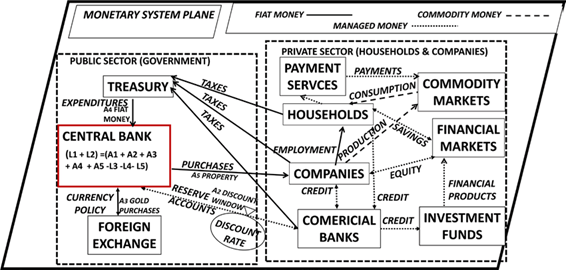
\includegraphics[width = 0.85\textwidth]{fin_system.png}

\end{frame}


\begin{frame}[fragile]{Unified Ledger}

\centering
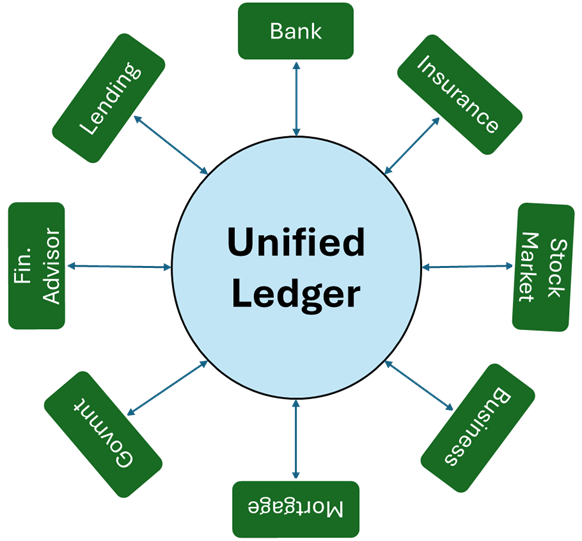
\includegraphics[width = 0.55\textwidth]{unified_ledger.png}

\end{frame}



%%%%%%%%%%%%%%%%%%%%%%%%%%%%%%%%%%%%

\begin{frame}[fragile]{Governance of the Unified Ledger}

\begin{itemize}
    \item Who should be in charge of such a unified ledger?
    \begin{itemize}
        \item Own
        \item Read
        \item Write
    \end{itemize}
\end{itemize}
\pause
\vspace{1cm}
\centering
\begin{tabular}{ccc}
 
\includegraphics[width = 3cm]{us_logo.png} \hspace{.1cm} \pause  &  
\includegraphics[width = 3.5cm]{bigtech.png} \hspace{.1cm} \pause & 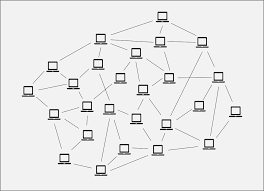
\includegraphics[width = 3.5cm]{network.png}
\end{tabular}

\end{frame}



%%%%%%%%%%%%%%%%%%%%%%%%%%%%%%%%%%%%


\begin{frame}[fragile]{Two Types of Network Decentralization}

\begin{tabular}{|p{4cm} |@{\hspace{1cm}} | p{4cm}|} % Two paragraph columns, each 5cm wide
    \cline{1-1} \cline{2-2}
     \textbf{Operational} & \textbf{Governance} \\ 
       \cline{1-1}\cline{2-2}

  %  \rowcolor{white} % Apply white background to the second row (optional, as it's default)
     \begin{itemize}
        \item Failure, attack, and censorship resistant
        \item Consensus mechanism (PoW, PoS, ...)
    \end{itemize}
    &
    \begin{itemize}
        \item Protocol rules
        \item Updates to the protocol
    \end{itemize} \\
    \cline{1-1}\cline{2-2}
\end{tabular}


\end{frame}





%%%%%%%%%%%%%%%%%%%%%%%%%%%%%%%%%%%%%%%%%%%%%%%%%%%%%%%%%%%%%%%%
%%%%%%%%%%%%%%%%%%%%%%%%%%%%%%%%%%%%%%%%%%%%%%%%%%%%%%%%%%%%%%%%
\section{What Are Open Source Communities?}
%%%%%%%%%%%%%%%%%%%%%%%%%%%%%%%%%%%%%%%%%%%%%%%%%%%%%%%%%%%%%%%%

\begin{frame}[fragile]{Close vs Open-sourcing Communities: a third way of governance. Lerner and Tirole (2005).}

\includegraphics[width = \textwidth]{Presentations/coase_linux.png}

\end{frame}

\begin{comment}
Talk about Coase 1937: boundaries of the firm are determined by transaction costs: 
Issue of Arms length negotiation: 
    - Price Discovery
    - Contract negotiation
    - Incomplete contracts
    - Inability to commit to long term contract

Issue with Firms
    - Organizational complexity costs
    - agency
    - Resource allocation inefficiency (no price mechanism)

Open source communities (like Linux) do not follow this framework. It is a third way. 

What are open source communities? Communities that come together to work on solving a specific project. Almost always a software. No owners. No formal company nor organization. No CEOs, board of directors, nor employees. Often there is no hierarchy within the community. No voting. The product is free, and open sourced. There are no financial statements. No profits. 

\end{comment}


%%%%%%%%%%%%%%%%%%%%%%%%%%%%%%%%%%%%%%%%%%%%%%%%%%%%%%%%%%%%%%%%

\begin{frame}[fragile]{Decision making in open source communities}

\large
\begin{quote}
    ``We reject: kings, presidents, and voting. We believe in:
rough consensus and running code.'' 
\begin{flushright}
    David Clark -- IETF, 1992
\end{flushright}
\end{quote}


\end{frame}

 
\begin{comment}
How do OSC make decisions? 

Rough Consensus: 
- Anyone can make proposals
- proposals are advanced and finalized only when a large number of participants agree, and there is a general sense that the concerns of the dissenting party have been heard and considered. 
- It's essentially an agreement that is "good enough" and can move forward without full agreement from all parties involved. 
- This approach allows for progress despite the presence of minor unresolved objections.

Running Code: 
- multiple actual and interoperable implementations of a proposed standard
must exist and be demonstrated before the proposal can be advanced along the standards
track.

No voting, otherwise sybil attack. 
\end{comment}

%%%%%%%%%%%%%%%%%%%%%%%%%%%%%%%%%%%%%%%%%%%%%%%%%%%%%%%%%%%%%%%%

\begin{frame}[fragile]{Example of open-sourcing communities.}

\includegraphics[width = \textwidth]{Presentations/open-source-community.png}

\end{frame}


%%%%%%%%%%%%%%%%%%%%%%%%%%%%%%%%%%%%%%%%%%%%%%%%%%%%%%%%%%%%%%%%

\begin{frame}[fragile]{Incentives in open source communities.}

\includegraphics[width = \textwidth]{Presentations/ibm_geek.jpg}

\end{frame}


\begin{comment}

All contributors involved in OSC are volunteers, not paid. Why do they do it? 

Two types: 
- Independent contributors. Skill building. Labor market signaling. Identity/Believing in the cause. BUt give up opportunity costs. 

- Affiliated companies: Establishing standards that are a better fit to their products/technology. Getting knowhow to then sell interface products. 

\end{comment}



%%%%%%%%%%%%%%%%%%%%%%%%%%%%%%%%%%%%%%%%%%%%%%%%%%%%%%%%%%%%%%%%

\begin{frame}[fragile]{Cryptocurrencies are all open-sourced communities...}

\includegraphics[width = \textwidth]{Presentations/cryptos.png}
\end{frame}


%%%%%%%%%%%%%%%%%%%%%%%%%%%%%%%%%%%%%%%%%%%%%%%%%%%%%%%%%%%%%%%%

\begin{frame}[fragile]{...but with a new set of incentives/market structure.}

\begin{itemize}
    \fitem Regulatory challenges.
    \fitem Publicly listed tokens (pricing/incentives).
    \fitem Market size.
\end{itemize}

\end{frame}


\begin{comment}

- Most crypto applications focus on financial services, a heavily regulated sector. How do regulators deal with a system where there are no companies, CEOs, responsible individuals, financial statements? 

- The presence of a token might align the behavior of contributors towards a common goal. Less dependend on outside support from companies.  It also provides a market pricing feedback. 

- Market size is \$1.4T. This is the largest experiment in OSC that has ever been attempted.  

\end{comment}


%%%%%%%%%%%%%%%%%%%%%%%%%%%%%%%%%%%%%%%%%%%%%%%%%%%%%%%%%%%%%%%%
\section{What is Ethereum?}
%%%%%%%%%%%%%%%%%%%%%%%%%%%%%%%%%%%%%%%%%%%%%%%%%%%%%%%%%%%%%%%%

\begin{frame}[fragile]{Ethereum is the most widely used programmable permissionless blockchain}

\includegraphics[width = \textwidth]{Presentations/eth_network.png} 

\end{frame}


\begin{comment}

Ethereum is the most widely used programmable permissionless blockchain: 

Let's unpack these three terms: Blockchain. Permissionless. Programmable. 

Blockchain: The idea is to have a network of computers, all running a compatible software called client), and they interact with each other. Differently from the internet, the P2P network not only relay information, but more importantly, comes to a consensus about whether transactions are valid or not. Several consensus mechanisms are used in crypto: PoW, PoS, BFT, ... .Ethereum switched from PoW to PoS last year. 

Permissionless: Anyone in the world can run the code, and interact in the P2P, by relaying transactions, and even participating in the consensus process. Anyone in the world can transact with anyone else. 

Programmable: Ethereum was the first crypto that used smart contracts. i.e. software that can be executed by nodes. For example, you and I can enter into a contracts that executes if certain conditions are fulfilled. Seems simple, but this conditional transaction spurred the birth of running software on the ethereum protocol. Ethereum is an worldwide, decentralized internet computer not owned nor controlled by anyone. 

\end{comment}

%%%%%%%%%%%%%%%%%%%%%%%%%%%%%%%%%%%%%%%%%%%%%%%%%%%%%%%%%%%%%%%%

\begin{frame}[fragile]{Blockchain Layers}

\includegraphics[width = \textwidth]{Presentations/layers.png} 

\end{frame}


\begin{comment}

Ethereum is thus one of the base layers on top of which software runs to provide services to users that access services using their crypto wallets. For exampe, uniswap provides token swaps. Compound provides overcollateralized borrowing and lending. Chainlink offers oracles that bring off-chain information on-chain.  Makerdao offers crypto-backed stablecoins. 

Ethereum is not the only base layers that offer a global internet computer. Many (too many) others exist. Actually, in my view, there has been overinvestment in base layers, and not enough on application layers.  

GO BACK ONE PAGE, AND SHOW the ETH NETWORK AGAIN: 

Now, usually when people talk about decentralization, they talk about the decentralization of the consensus process (51% attack,...). For good reason, it is a very important topic in blockchain, because there is no centralized entity, and at its core, the purpose of a blockhain is to validate (conditional) transactions. 

In this paper, we do not want to talk about the decentalization of the consensus protocol, but about something equally important, but less studied: the decentralization of the Ethereum governance. Ethereum has been evolving over time, to make the protocol faster, more energy efficient, more decentralized.

\end{comment}


%%%%%%%%%%%%%%%%%%%%%%%%%%%%%%%%%%%%%%%%%%%%%%%%%%%%%%%%%%%%%%%%

\begin{frame}[fragile]{In this paper, we embark on a comprehensive exploration of Ethereum's governance.}

\begin{itemize}
    \fitem  How are protocol enhancements are proposed, reviewed, finalized, implemented, and adopted? 
    \fitem How decentralized is Ethereum governance? Which entities exert the greatest influence? How transparent is the governance process?
    \fitem Does governance matter for Ether token price?
\end{itemize}

\end{frame}


\begin{comment}


\end{comment}

%%%%%%%%%%%%%%%%%%%%%%%%%%%%%%%%%%%%%%%%%%%%%%%%%%%%%%%%%%%%%%%%

\begin{frame}[fragile]{Why is governance decentralization important? }

\centering
\vspace{-1cm}
\includegraphics[width = 0.5\textwidth]{Presentations/mission.png} 


\includegraphics[width = \textwidth]{Presentations/liability_insider.png} 

\end{frame}


\begin{comment}

If you think about the mission of the SEC, it is : (i) protect investors (ii) maintain a fair, orderly, and efficient financial markets. (iii) Facilitate capital formation. 

To accomplish this mission, the SEC specifies rules about registering securities, with related duties to disclose information to the public for a number of reasons. To enforce such rules, the agency has to identify responsible individuals who are required to make disclosure statements. 

For example, assigning liability if something goes wrong. Have fair markets with a disclosure regime that prevents insider trading and information. and prevent contagion and systemic risks. 
\end{comment}



%%%%%%%%%%%%%%%%%%%%%%%%%%%%%%%%%%%%%%%%%%%%%%%%%%%%%%%%%%%%%%%%

\begin{frame}[fragile]{1946 Orange Groves in Florida and Crypto}
\centering

\includegraphics[width = 0.5\textwidth]{Presentations/howey.png} 

\end{frame}


\begin{comment}

Why does the SEC care so much about crypto, and not Linux, or Mozzilla?

It obviously hinges on the definition of security, and whether cryptocurrencies are indeed securities. 

This is William John Howey. I don't want to engage in a lenghty legal discussion on whether or when crytpo is a security or not, but the main test to determine that is the Howey Test, which has four legs: (i) an investment of money/value (ii) in a common enterprise (iii) with an expectation of profit (iv) derived from the effort of others. 

The last leg has to do with how decentralized the goverance process truly is. if it is truly decentralized, noone has any insider information, and thus the disclosure requirement are not needed. 


\end{comment}


%%%%%%%%%%%%%%%%%%%%%%%%%%%%%%%%%%%%%%%%%%%%%%%%%%%%%%%%%%%%%%%%

\begin{frame}[fragile]{Is crypto governance truly decentralized? }

\includegraphics[width = \textwidth]{Presentations/gary_satoshi.png} 

\end{frame}


\begin{comment}

There are two main camps: people that believe that crypto currencies are not really decentralized, but are centralized with clearly identifiable responsible individuals.   

And others that believe that they are fully decentralized, and noone is really in charge? 

Our paper will not answer this question. We are not lawyers, nor regulators. it is not our job to draw the line on whether it is decentralized "enough" or not. But what we can do is to provide evidence about the transparency and concentration of power in the ethereum governance process. To our knowledge, this is the first paper that provides a framework to evaluate the decentalization of ethereum's decision making process, the data, and the analysis. 

\end{comment}



%%%%%%%%%%%%%%%%%%%%%%%%%%%%%%%%%%%%%%%%%%%%%%%%%%%%%%%%%%%%%%%%
\section{How are decisions made in Ethereum?}
%%%%%%%%%%%%%%%%%%%%%%%%%%%%%%%%%%%%%%%%%%%%%%%%%%%%%%%%%%%%%%%%

 
%%%%%%%%%%%%%%%%%%%%%%%%%%%%%%%%%%%%%%%%%%%%%%%%%%%%%%%%%%%%%%%%

\begin{frame}[fragile]{Ethereum Governance}

\begin{itemize}
    \item Ethereum governance is based on governance systems in other
open source communities.
    \begin{itemize}
        \item No formal voting process on rule changes
        \item Idea to hear everyone out, find compromises and mitigate
concerns: rough consensus.
        \item But: Forking code base vs. forking state.
        \item Persistent chain splits and alternative protocol versions are
possible, but costly.
    \end{itemize}

\end{itemize}
\end{frame}


%%%%%%%%%%%%%%%%%%%%%%%%%%%%%%%%%%%%%%%%%%%%%%%%%%%%%%%%%%%%%%%%

\begin{frame}[fragile]{Ethereum Improvement Proposal (EIP) Process}

\includegraphics[width = \textwidth]{Figures/EIP_Process.png} 

\end{frame}


%%%%%%%%%%%%%%%%%%%%%%%%%%%%%%%%%%%%%%%%%%%%%%%%%%%%%%%

\begin{frame}{Empirical Analysis}
	\begin{enumerate}
		\item \textbf{Transparency and Openness}
		\begin{itemize}
			\item EIP Data
			\item Readability Scores
			\item Discussion Venue and Secondary Data
			\item Identities
		\end{itemize}
		\item \textbf{Centralization and Community Engagement}
		\begin{itemize}
			\item Authorship Concentration and Network Analysis
			\item Determinants of Community Engagement
			\item Company/Organization Affiliation
			\item Effect on Implementation and Adoption
			\item Client Development Concentration 
			\item Reverse Dependencies
		\end{itemize}
\color{black}
		\item \textbf{Governance Effect on Ether Price}
		\begin{itemize}
			\item AllCoreDevCall Decisions and Token Price
		\end{itemize}
\color{black}
	\end{enumerate}
\end{frame}

%%%%%%%%%%%%%%%%%%%%%%%%%%%%%%%%%%%%%%%%%%%%%%%%%%%%%%%%%%%%%%%%
\section{Transparency and Openness}
%%%%%%%%%%%%%%%%%%%%%%%%%%%%%%%%%%%%%%%%%%%%%%%%%%%%%%%%%%%%%%%%

%%%
\begin{frame}{EIP Production Over Time}

We collected data for all EIPs until June 21st, 2023. Note, that we have dropped \textit{Meta} and \textit{Info} EIPs from our dataset. Number of EIPs: 612. Number of unique authors: 689.

\begin{figure}
	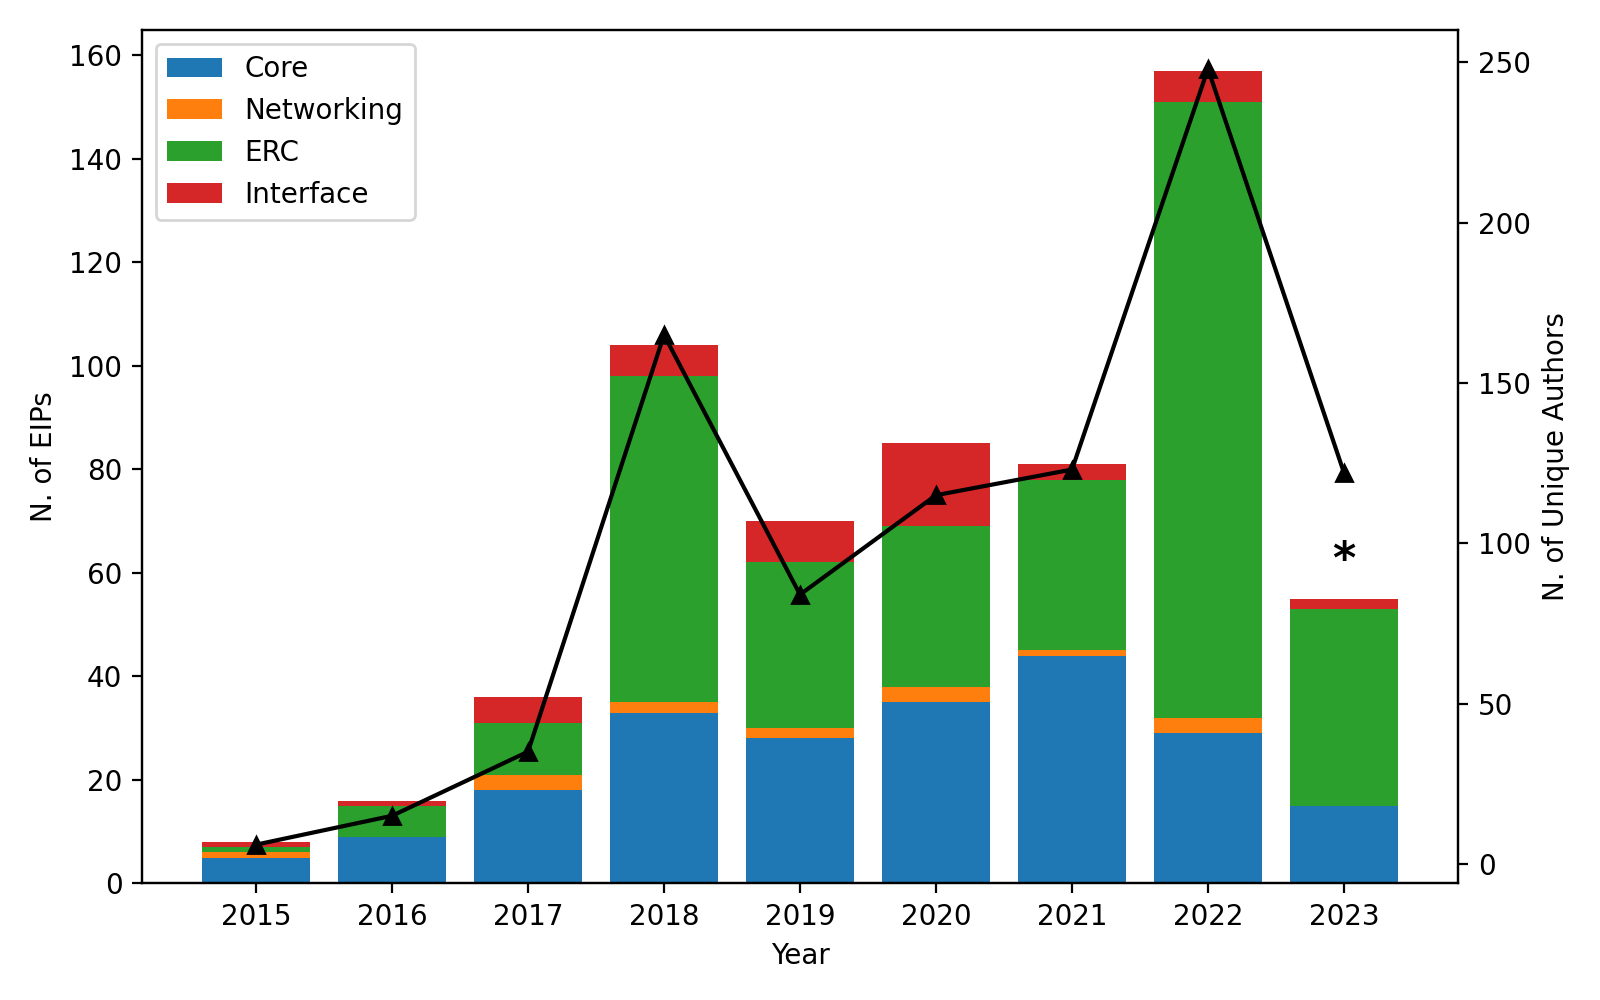
\includegraphics[width = 0.75\textwidth]{../Figures/neip_by_year.png}
    \caption{EIP production over time.}
\end{figure}
\end{frame}
%%%



%%%%%%%%%%%%%%%%%%%%%%%%%%%%%%%%%%%%%%%%%%%%%
\subsection{EIP Readability}
%%%%%%%%%%%%%%%%%%%%%%%%%%%%%%%%%%%%%%%%%%%%%
%%%
\begin{frame}{Flesch-Reading-Ease Score}
	Some initial evidence on the complexity of the data.\\

	
	\begin{figure}
		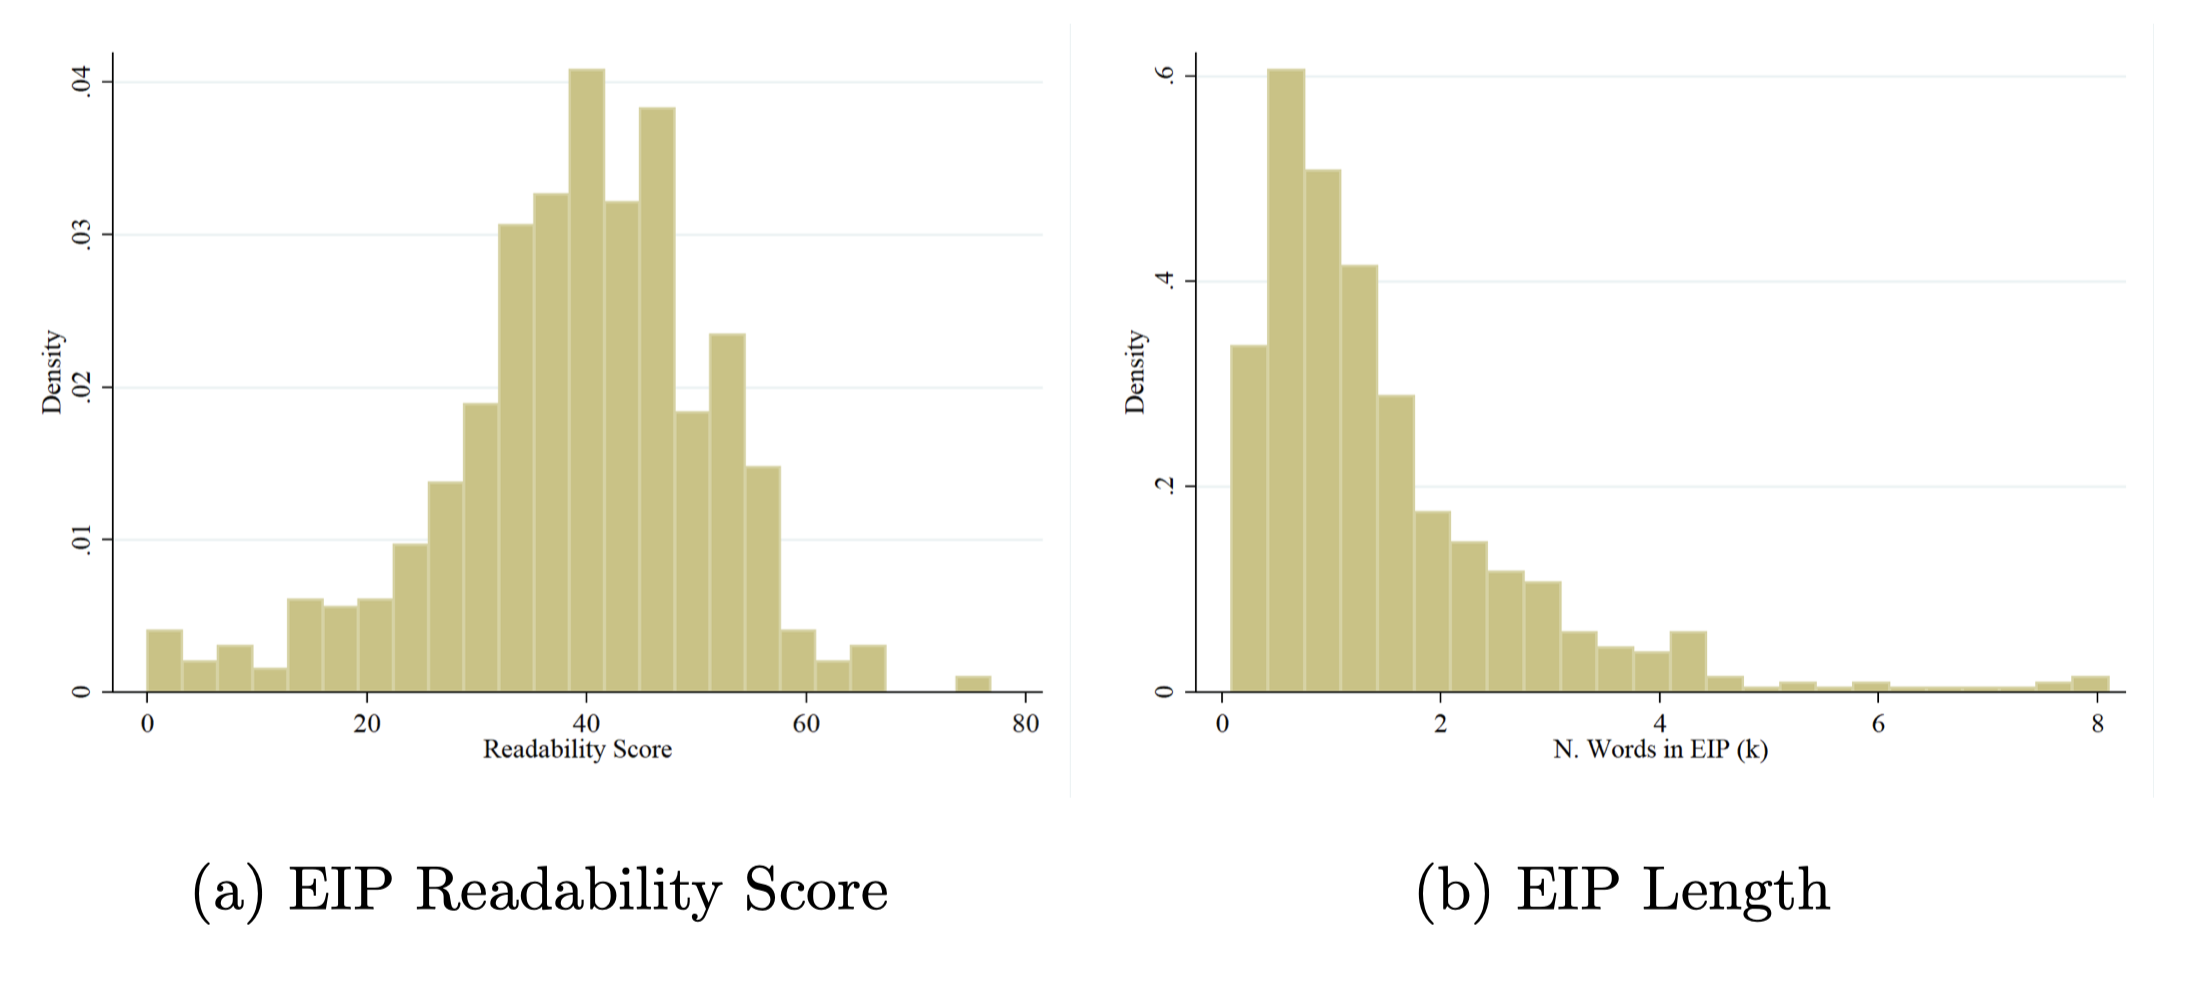
\includegraphics[width = \textwidth]{../Figures/readability.png}
		\caption{Readability score (a) and number of words (b). Readability score is based on sentence length (words) and word length (syllables). Score $\in [1,100]$, where 1 is least and 100 most readable. College level: 30-50. For reference, this paper: 43.5.}
	\end{figure}
	% Standard to evaluate readability. Uses word/sentence and syllables/word ratio with some constants.
	% Mention that this only reflects sentence structure. Effects of technical complexity will be considered later -> author diversity by EIP type.
	% Vast majority approximately college level, some much more complex.
	% On average 1000 words, 2-2.5 single-spaced pages 
\end{frame}
%%%

%%%%%%%%%%%%%%%%%%%%%%%%%%%%%%%%%%%%%%%%%%%%%
\subsection{EIP Discussion Venues}
%%%%%%%%%%%%%%%%%%%%%%%%%%%%%%%%%%%%%%%%%%%%%

%%%
\begin{frame}[fragile]{Github}
		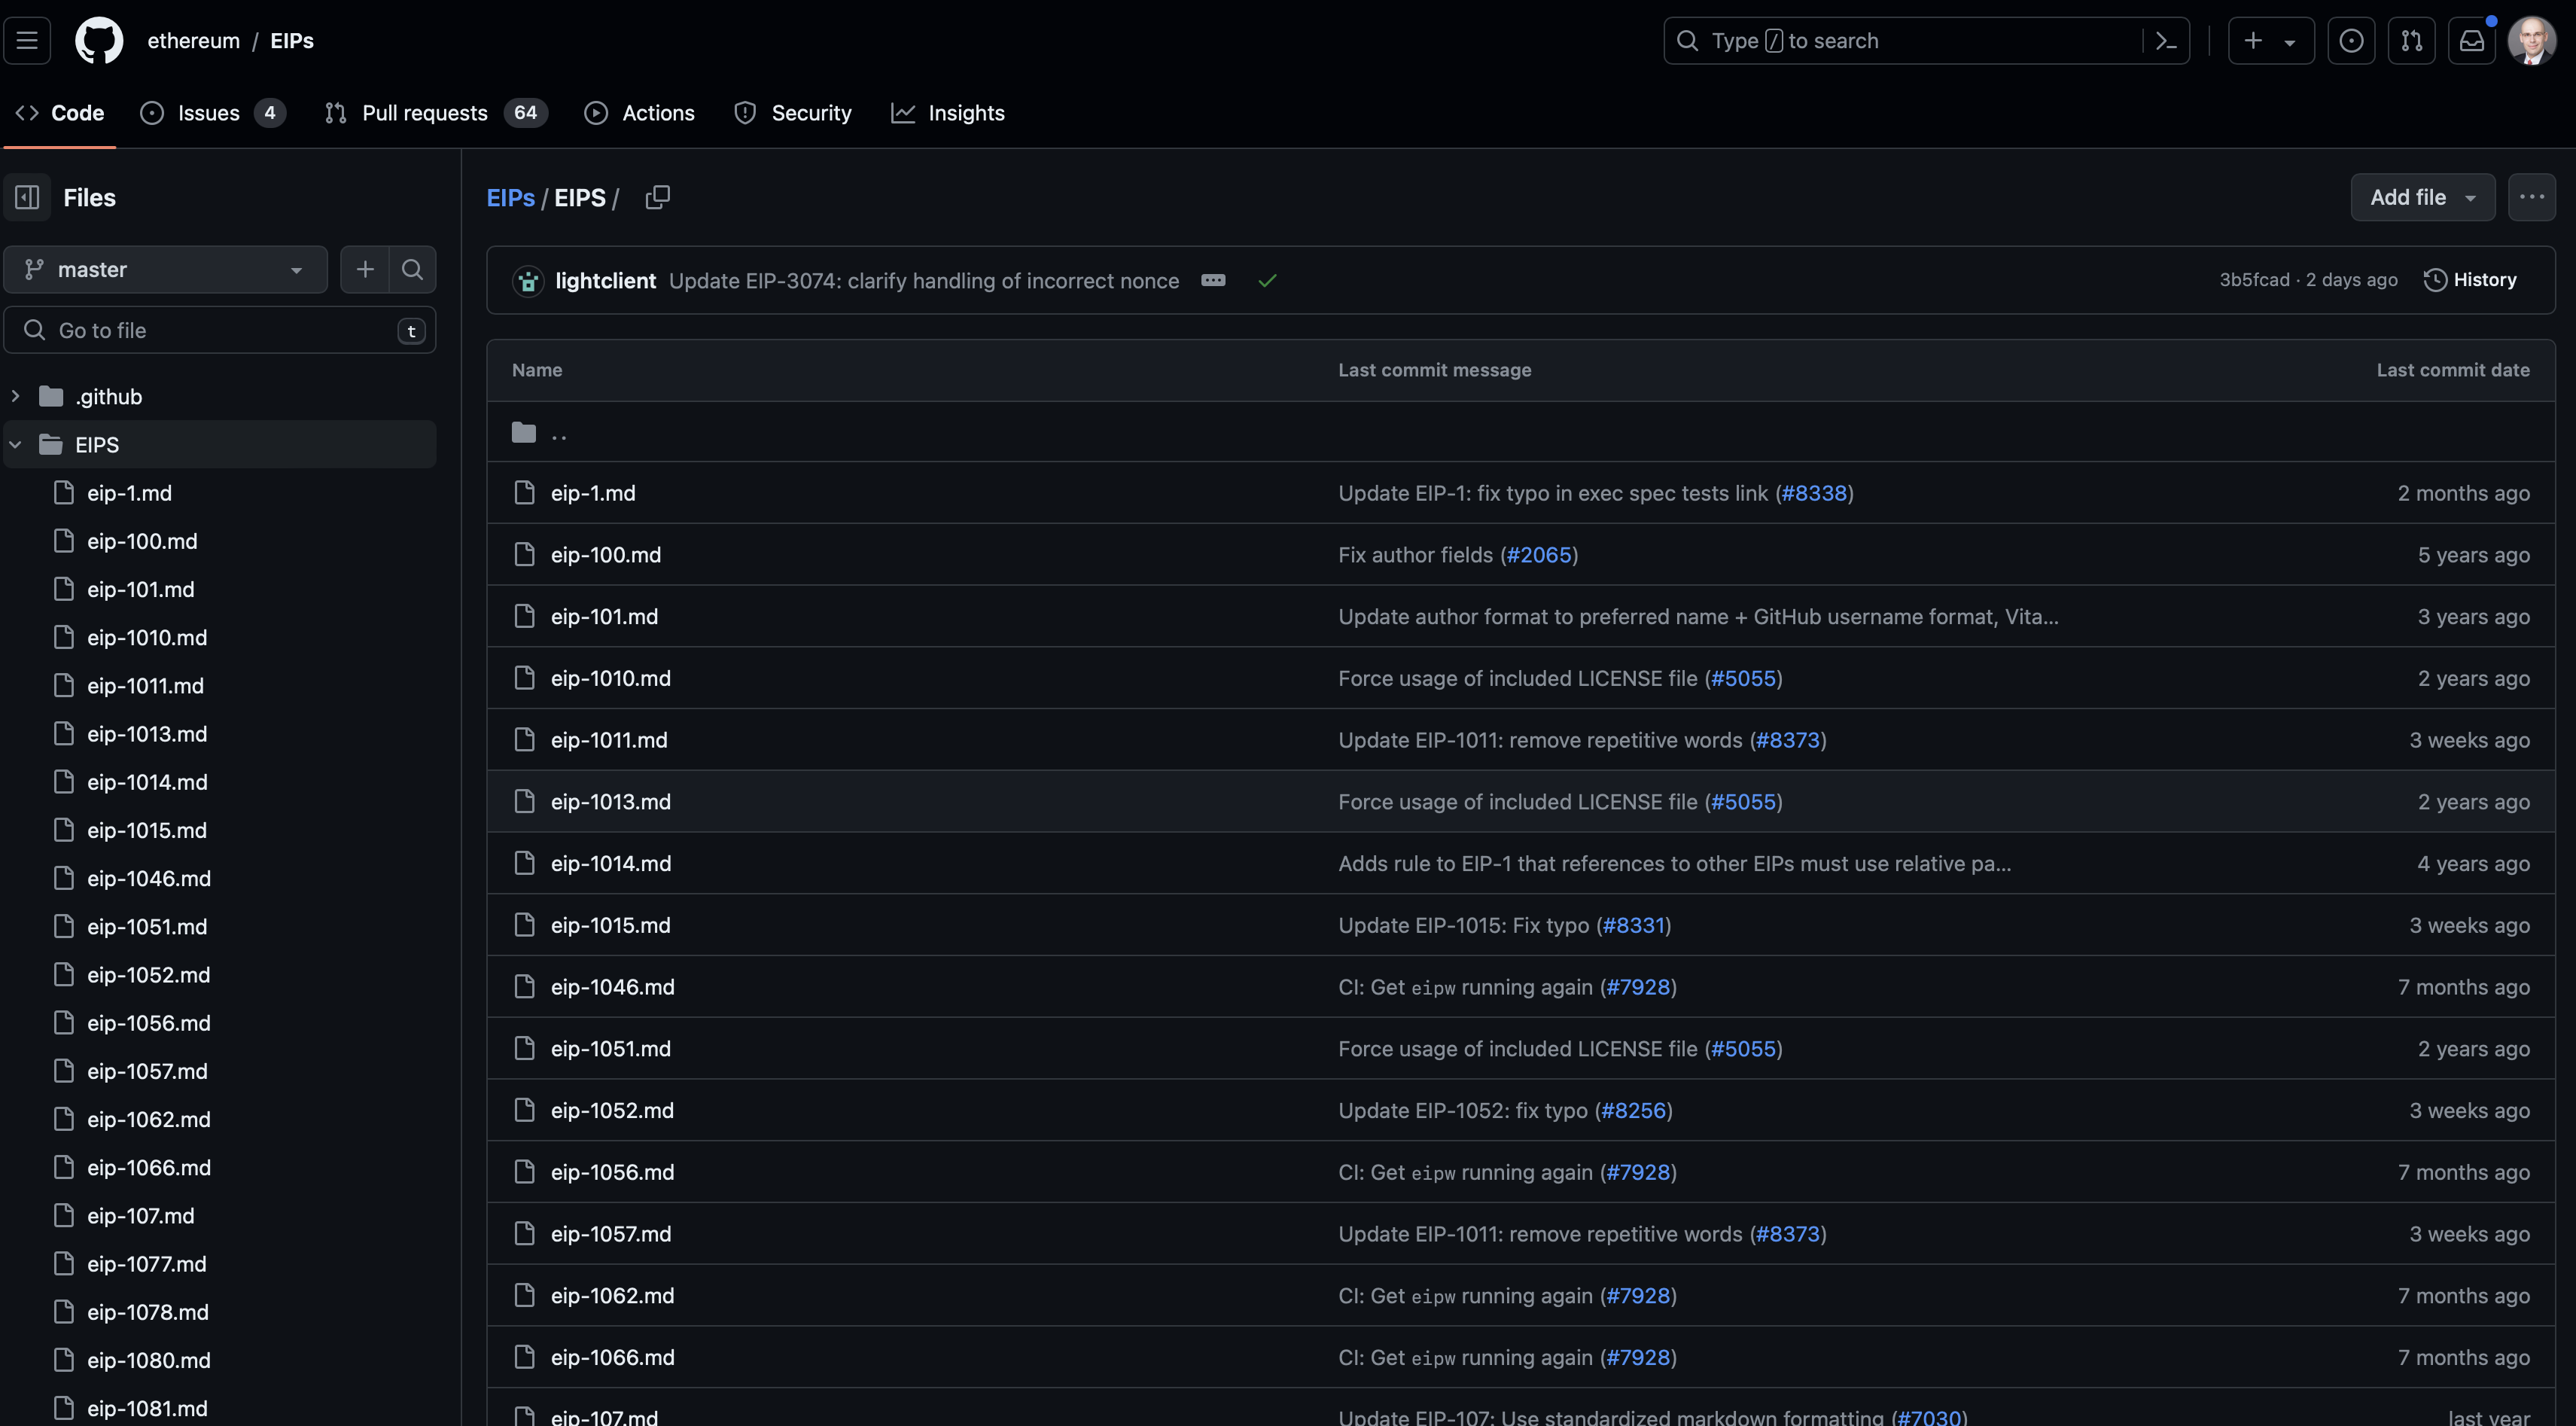
\includegraphics[width=\textwidth]{../Figures/githubEIPRepo.png}
\end{frame}
%%%

\iffalse
%%%
\begin{frame}[fragile]{Github Commits}
	\begin{figure}
		\includegraphics[width=0.9\textwidth]{../Figures/eipCommits.png}
		\caption{Number of Commits and Non-Author Influence}
	\end{figure}
\end{frame}
%%%
\fi

%%%
\begin{frame}{Fellowship of Ethereum Magicians (FEM)}
	\begin{figure}
		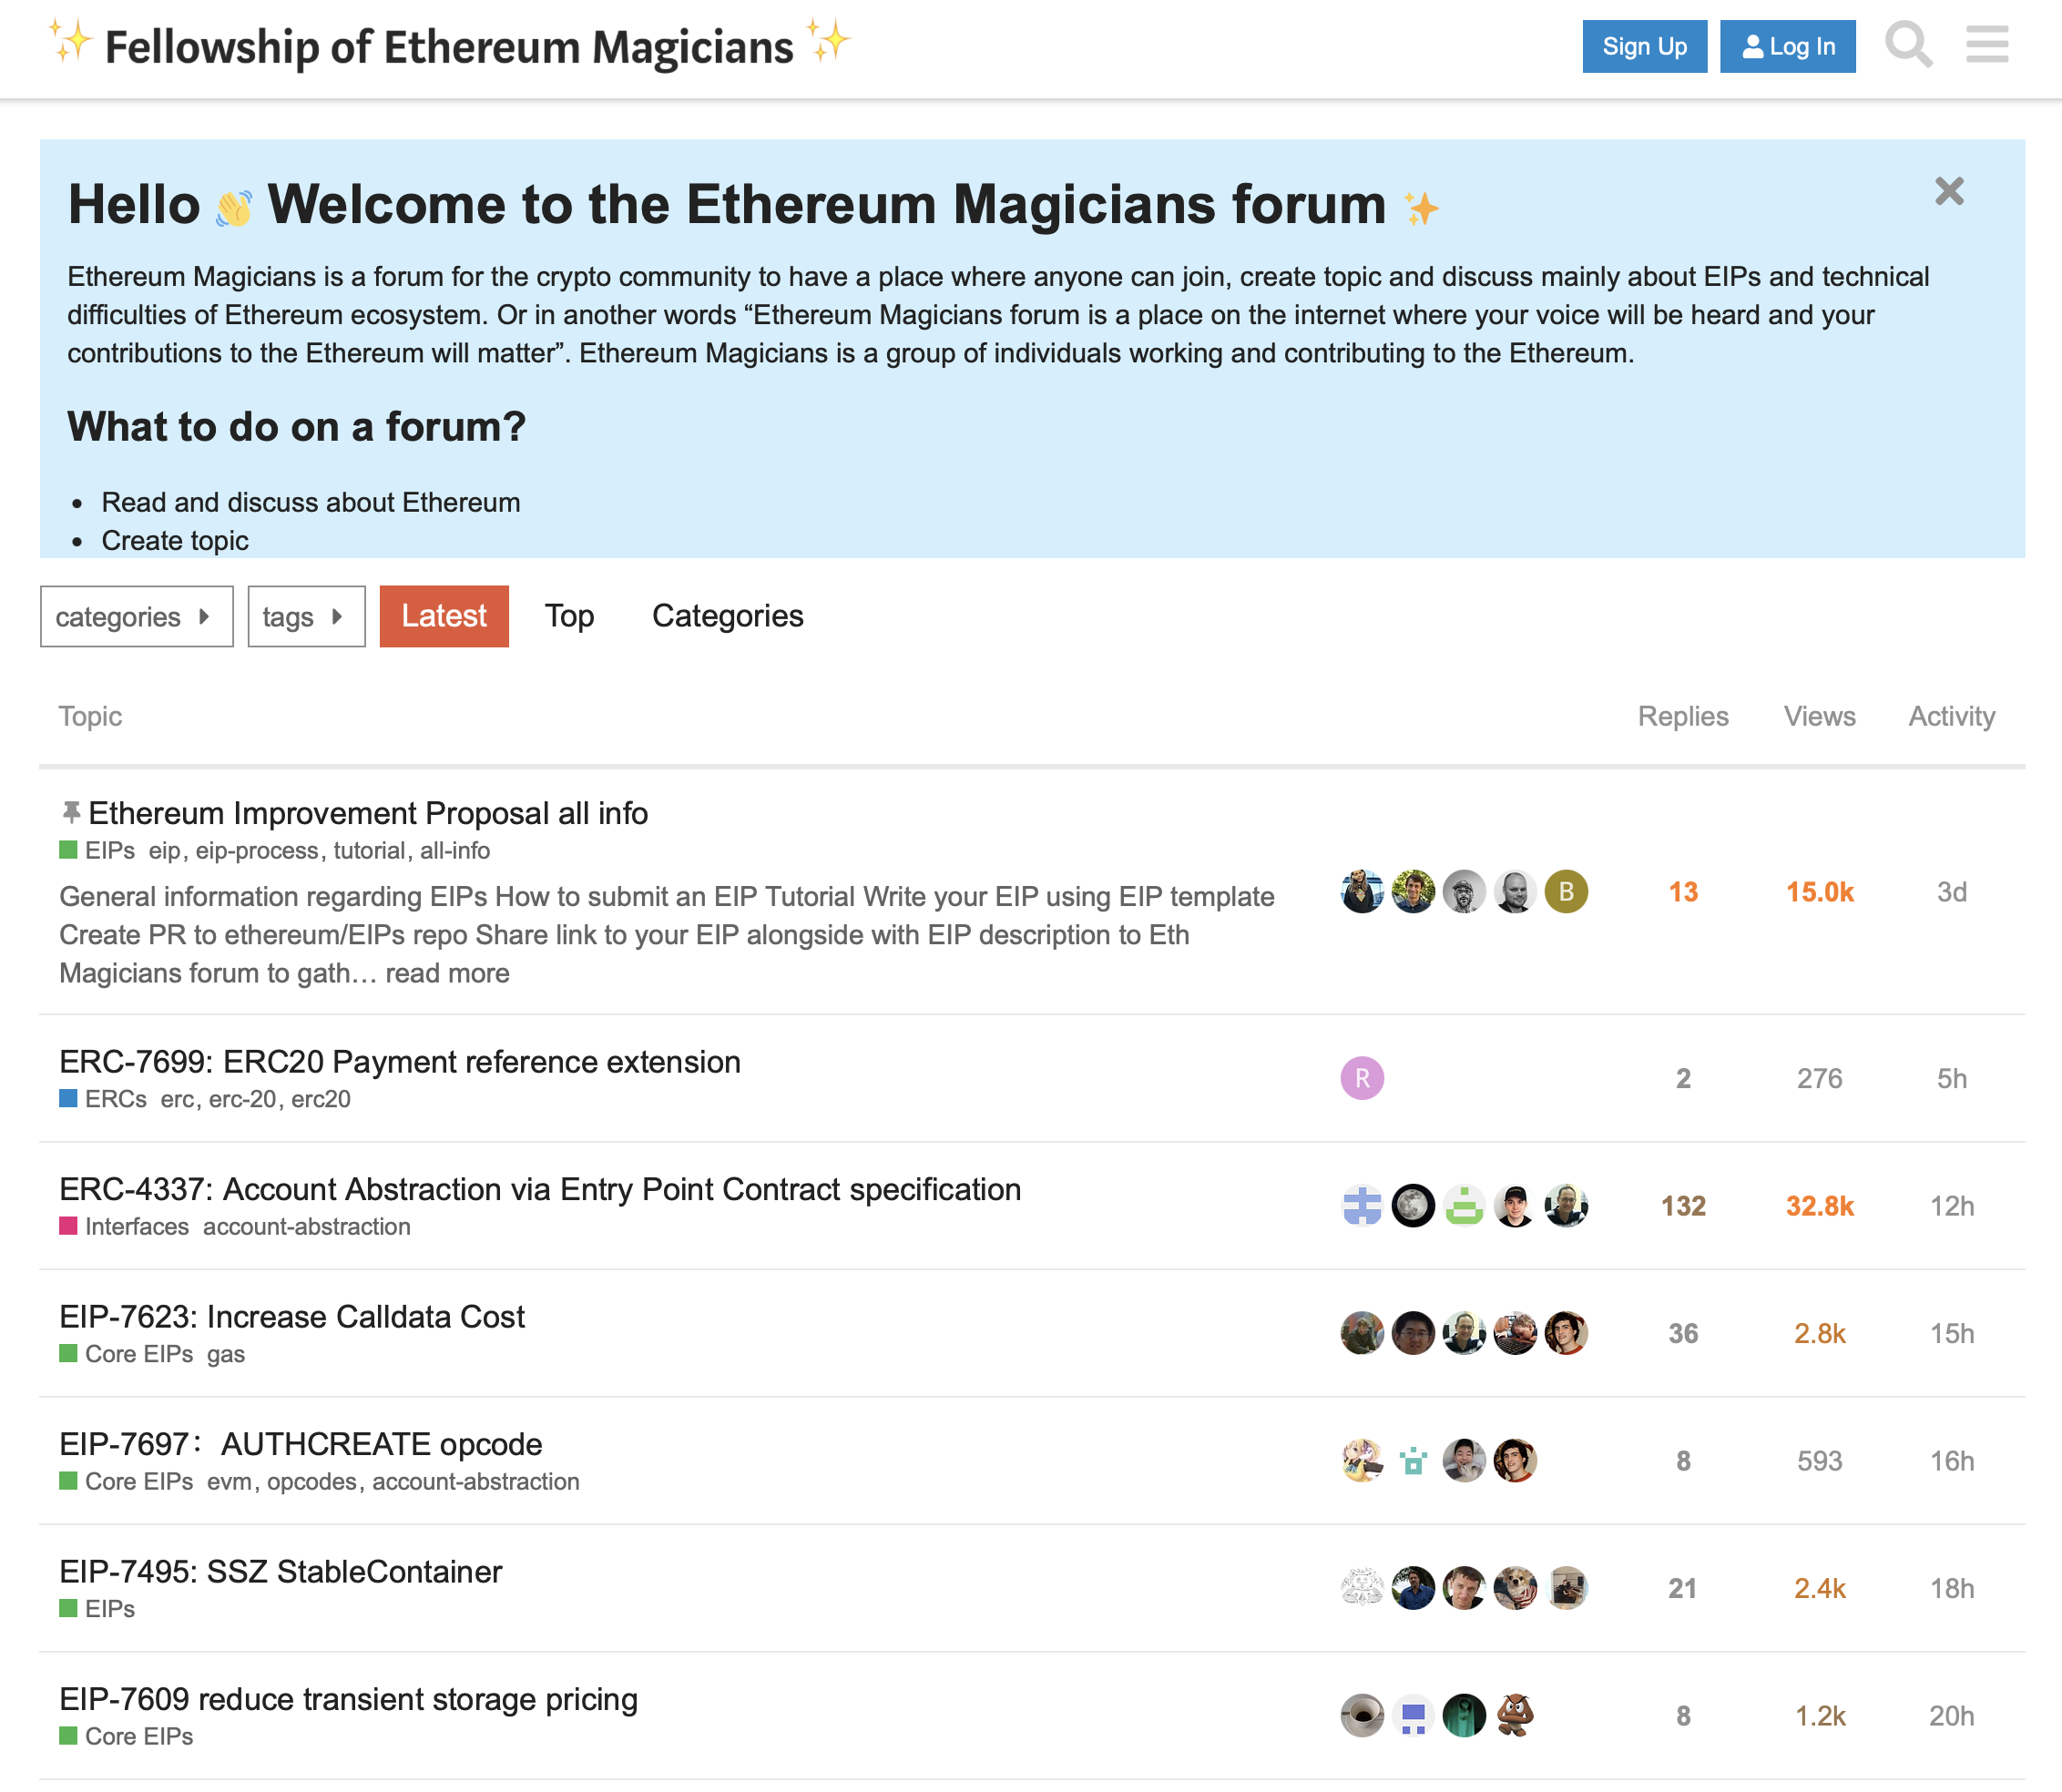
\includegraphics[width=0.8\textwidth]{../Figures/FEM.png}
	\end{figure}
	% So far, 1,101 individuals have contributed to these discussions, resulting in 1,6M views, 6,416 comments, and 4,675 likes.
\end{frame}
%%%

%%%
\begin{frame}{FEM Comments}
		\begin{figure}
		\includegraphics[width=\textwidth]{../Figures/FEMcombined.png}
		\caption{FEM views and adapted activity Lorenz curve.}
	\end{figure}
\end{frame}
%%%

%%%
\begin{frame}[fragile]{AllCoreDev Calls}
	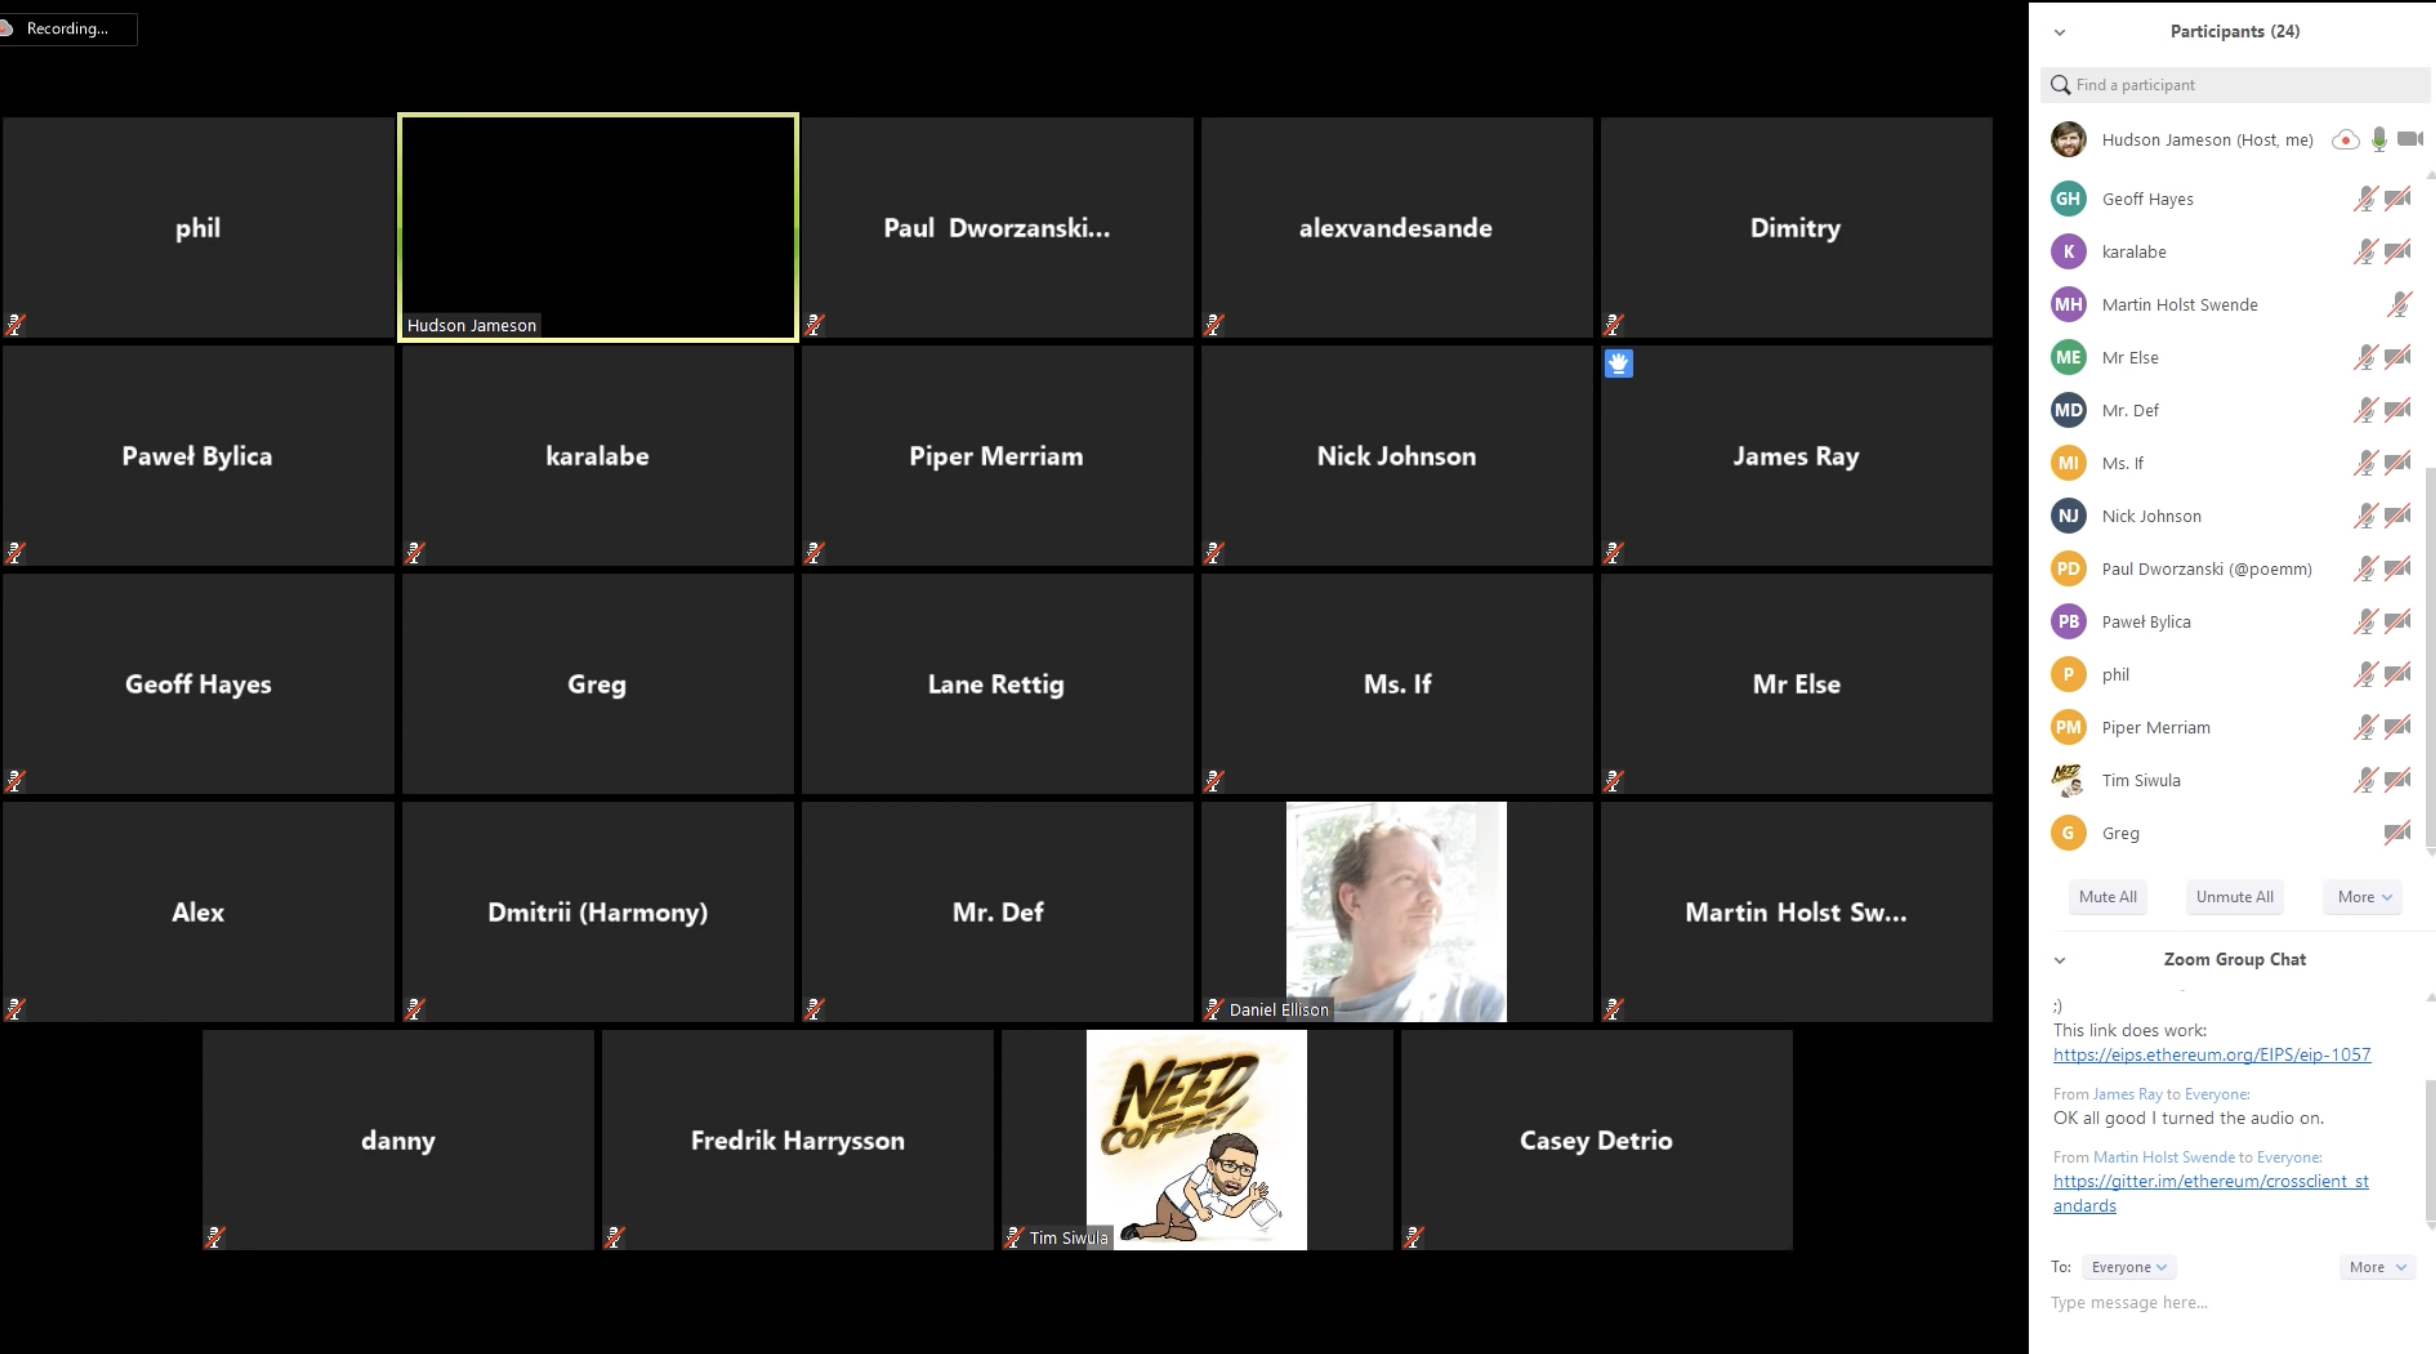
\includegraphics[width=\textwidth]{../Figures/allCoreDevCall.png}
\end{frame}
%%%

%%%
\begin{frame}{AllCoreDev Call Attendee Statistics}
	\begin{figure}
		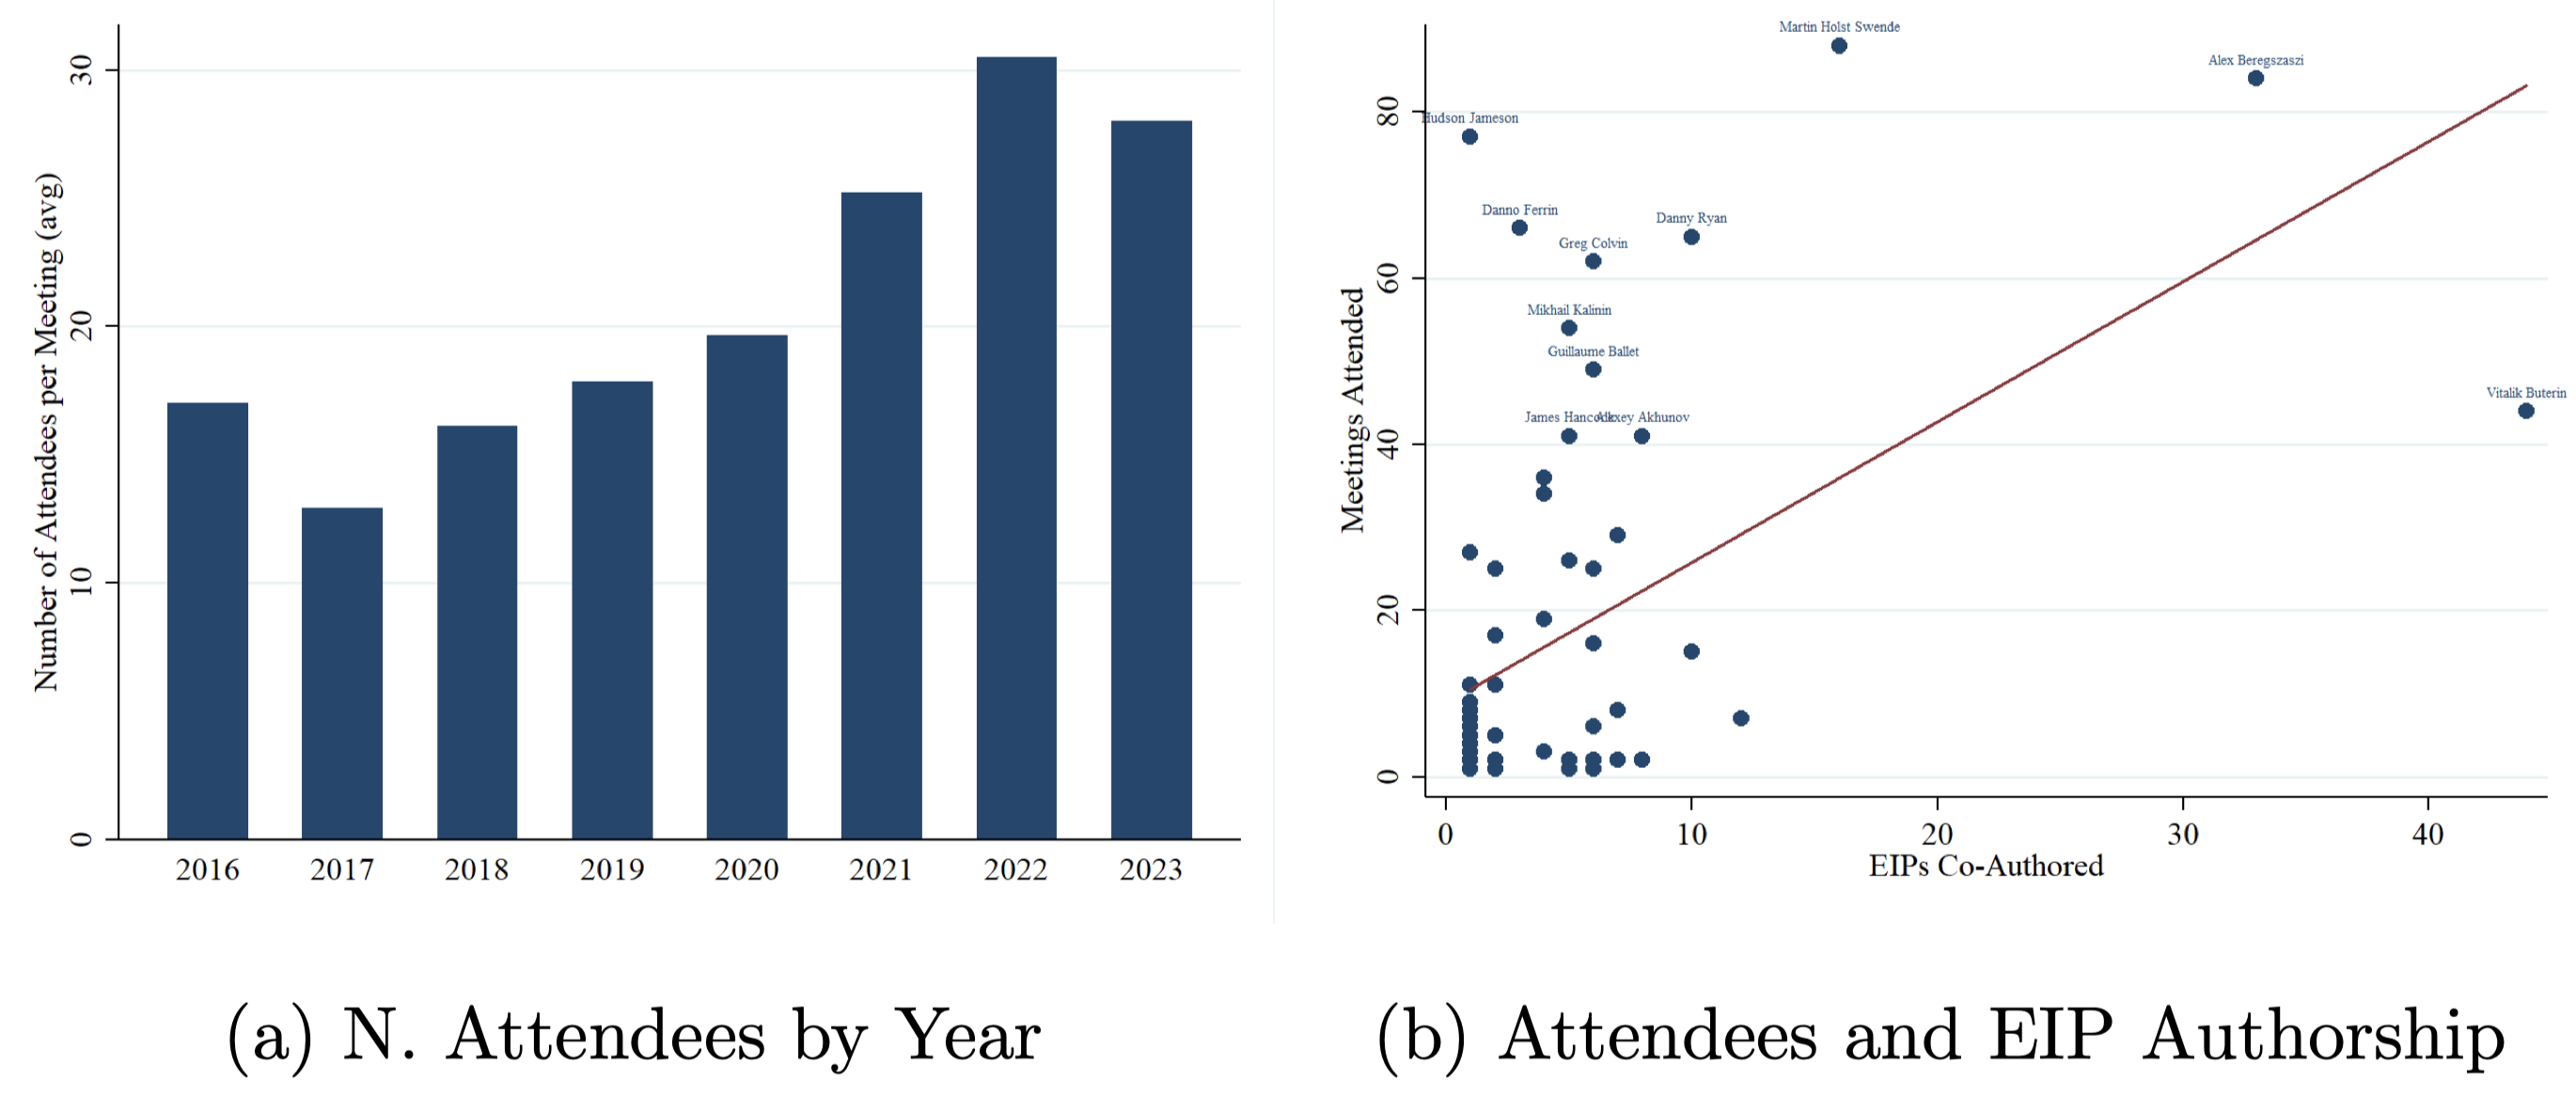
\includegraphics[width=0.9\textwidth]{../Figures/allCoreDevCallStats.png}
		\caption{AllCoreDevCalls Attendees}
	\end{figure}
\end{frame}
%%%


%%%%%%%%%%%%%%%%%%%%%%%%%%%%%%%%%%%%%%%%%%%%%
\subsection{Identities}
%%%%%%%%%%%%%%%%%%%%%%%%%%%%%%%%%%%%%%%%%%%%%
%%%
\begin{frame}{Anonymity}
	
	How many contributors disclose their true identity?\\
	
	\begin{itemize}
		\item Important to understand quality of the data
		\item Potentially important variable in our analysis (trust) 
		\item Used for affiliations and social media data. 
	\end{itemize}

\vspace{1em}

\uncover<2->{
\textbf{The majority of Ethereum contributors disclose their name:}
		\begin{itemize}
			\item \textbf{EIP Authors:} $\sim89\%$
			\item \textbf{AllCoreDev Call Participants:} $\sim79\%$
			\item \textbf{Top Client Developers:} $\sim79\%$
		\end{itemize}
		}
\end{frame}
%%%



%%%%%%%%%%%%%%%%%%%%%%%%%%%%%%%%%%%%%%%%%%%%%%%%%%%%%%%%%%%%%%%%
\section{Centralization and Community Engagement}
%%%%%%%%%%%%%%%%%%%%%%%%%%%%%%%%%%%%%%%%%%%%%%%%%%%%%%%%%%%%%%%%



%%%%%%%%%%%%%%%%%%%%%%%%%%%%%%%%%%%%%%%%%%%%%
\subsection{Influential Authors}
%%%%%%%%%%%%%%%%%%%%%%%%%%%%%%%%%%%%%%%%%%%%%

%%%
\begin{frame}{Influential EIP Authors}
	\begin{figure}
		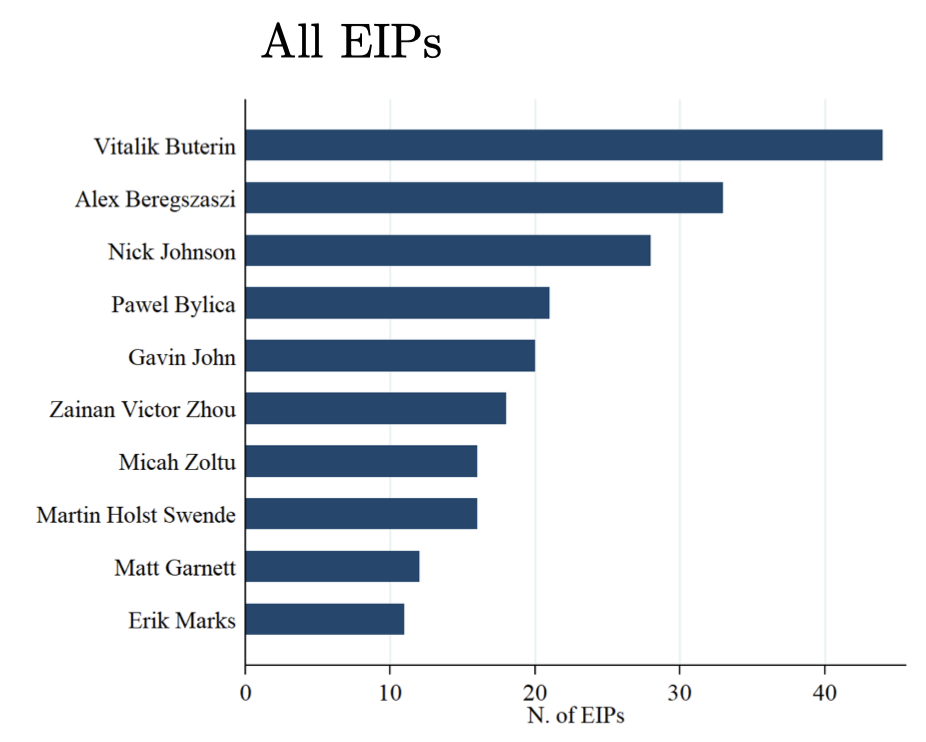
\includegraphics[width = 0.6\textwidth]{../Figures/top10AuthorsAll.png}
		\caption{Number of EIPs by authors (all categories).}
	\end{figure}
\end{frame}
%%%

%%%
\begin{frame}{Influential EIP Authors (ctd.)}
	\begin{figure}
		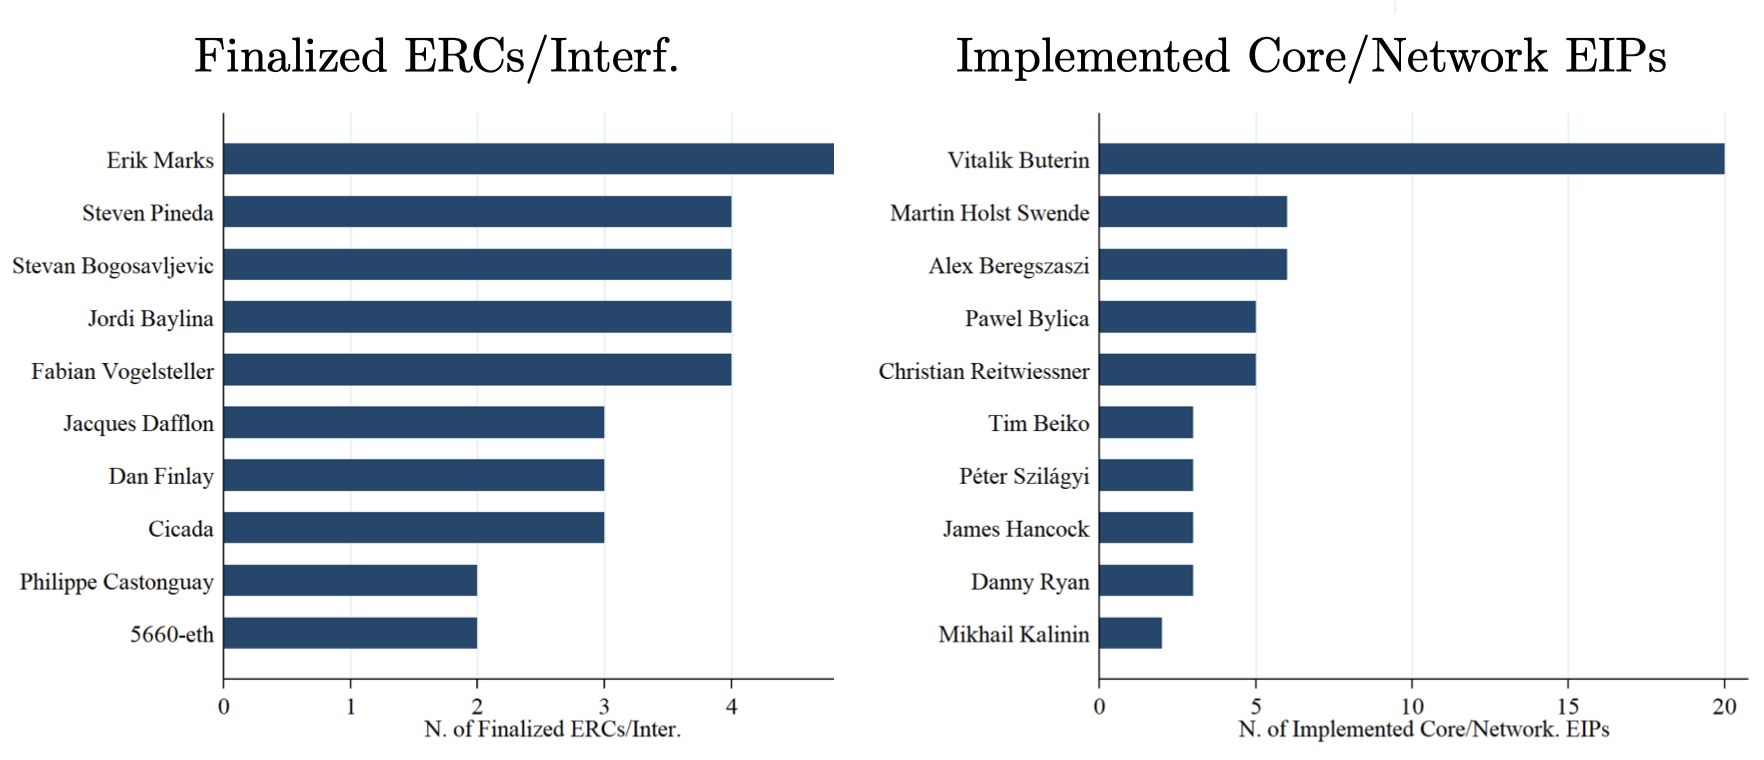
\includegraphics[width = \textwidth]{../Figures/top10AuthorsSplit.png}
		\caption{Number of EIPs by authors -- ERC/Interface (a) and Core/Network (b).}
	\end{figure}
\end{frame}
%%%

%%%
\begin{frame}{Authorship Concentration}
	\begin{figure}
		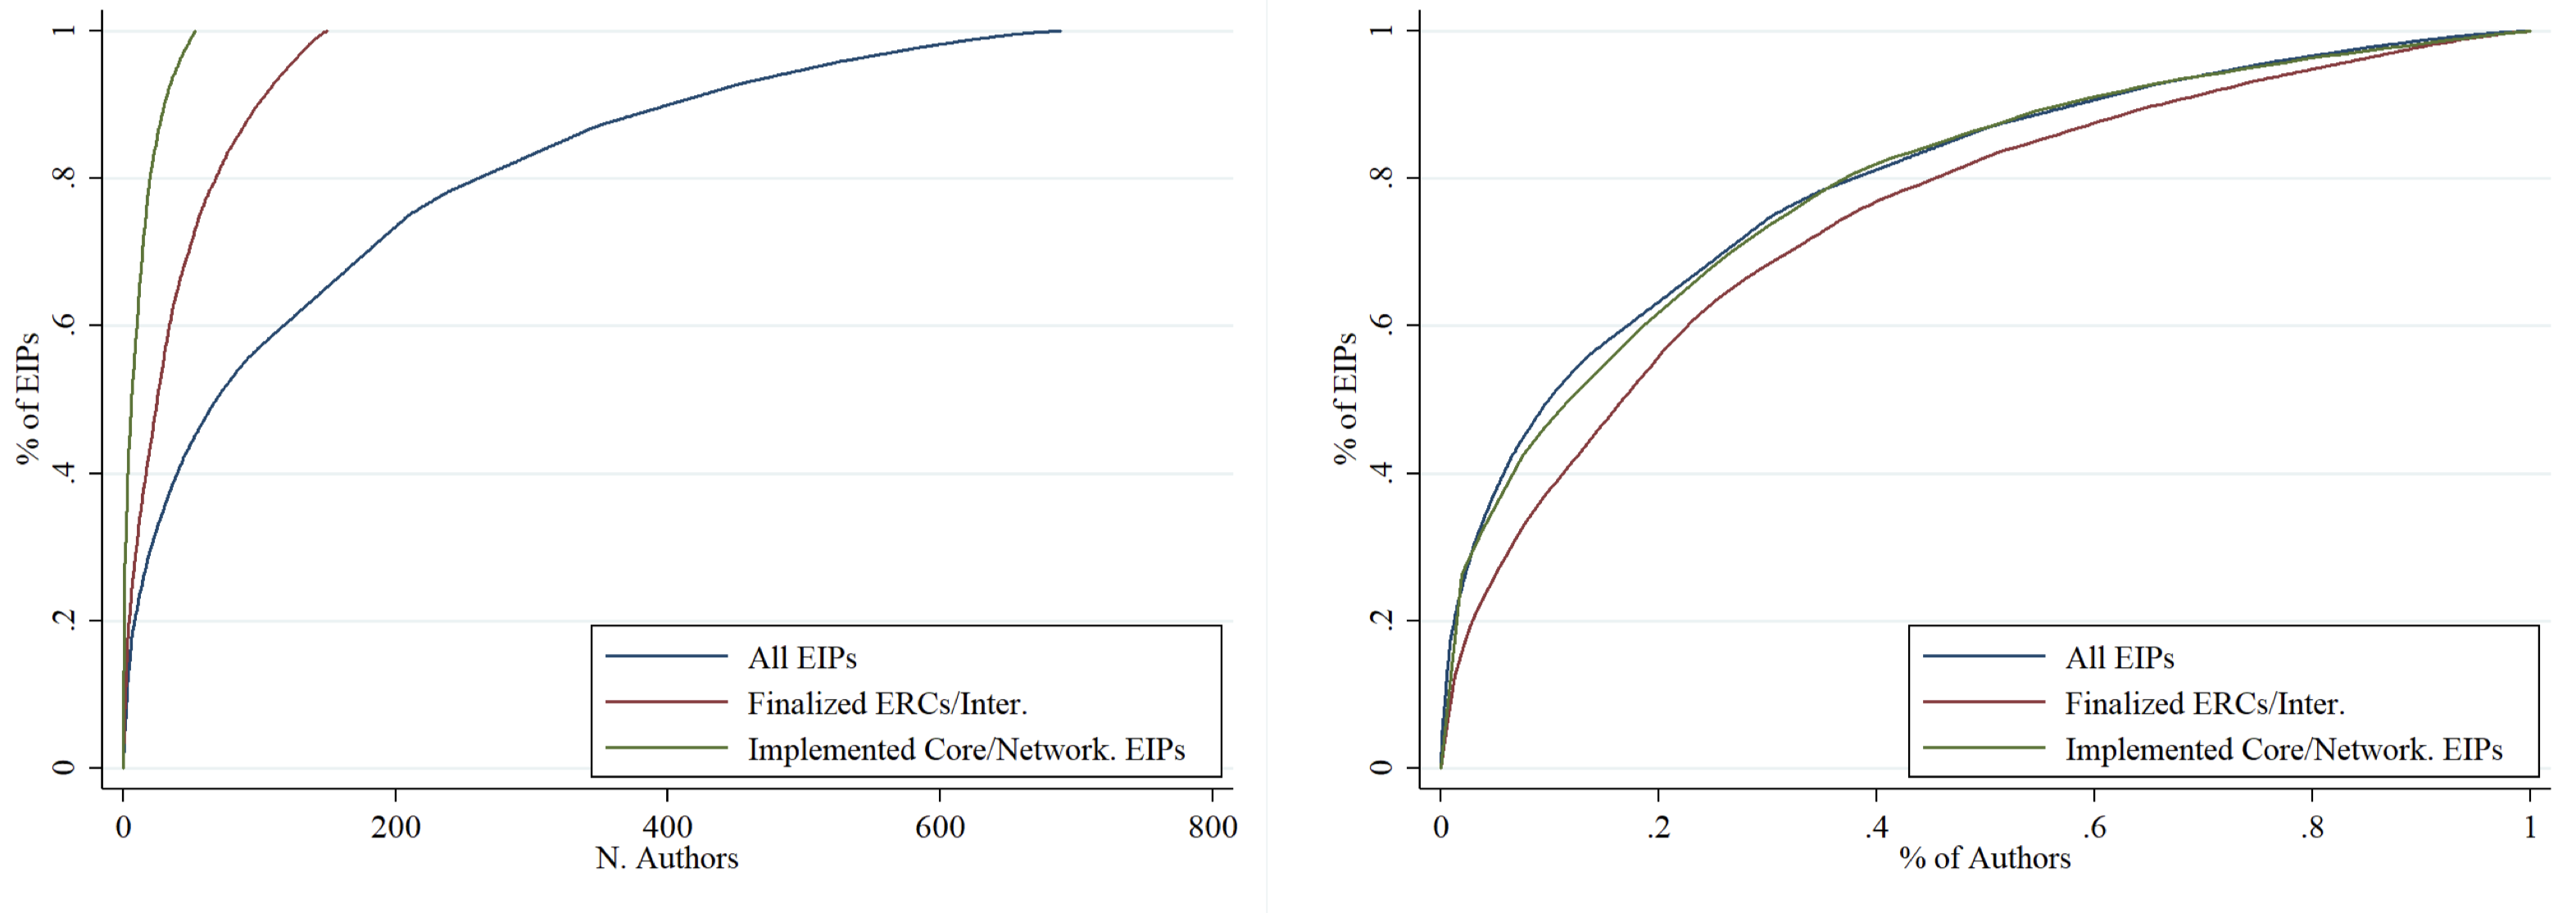
\includegraphics[width = \textwidth]{../Figures/authorLorenzCurve.png}
		\caption{EIP authorship concentration -- absolute (a) and relative (b).}
	\end{figure}
	\footnotesize
	The top 10 authors produced:
	\begin{itemize}
		\item $\sim$ 21\% of all EIPS.
		\item $\sim$ 29\% of all finalized ERC/Interface EIPs.
		\item $\sim$ 68\% of all implemented Core/networking EIPs.
	\end{itemize}
\end{frame}
%%%

%%%
\begin{frame}{Authorship Concentration Over Time}
	\begin{figure}
		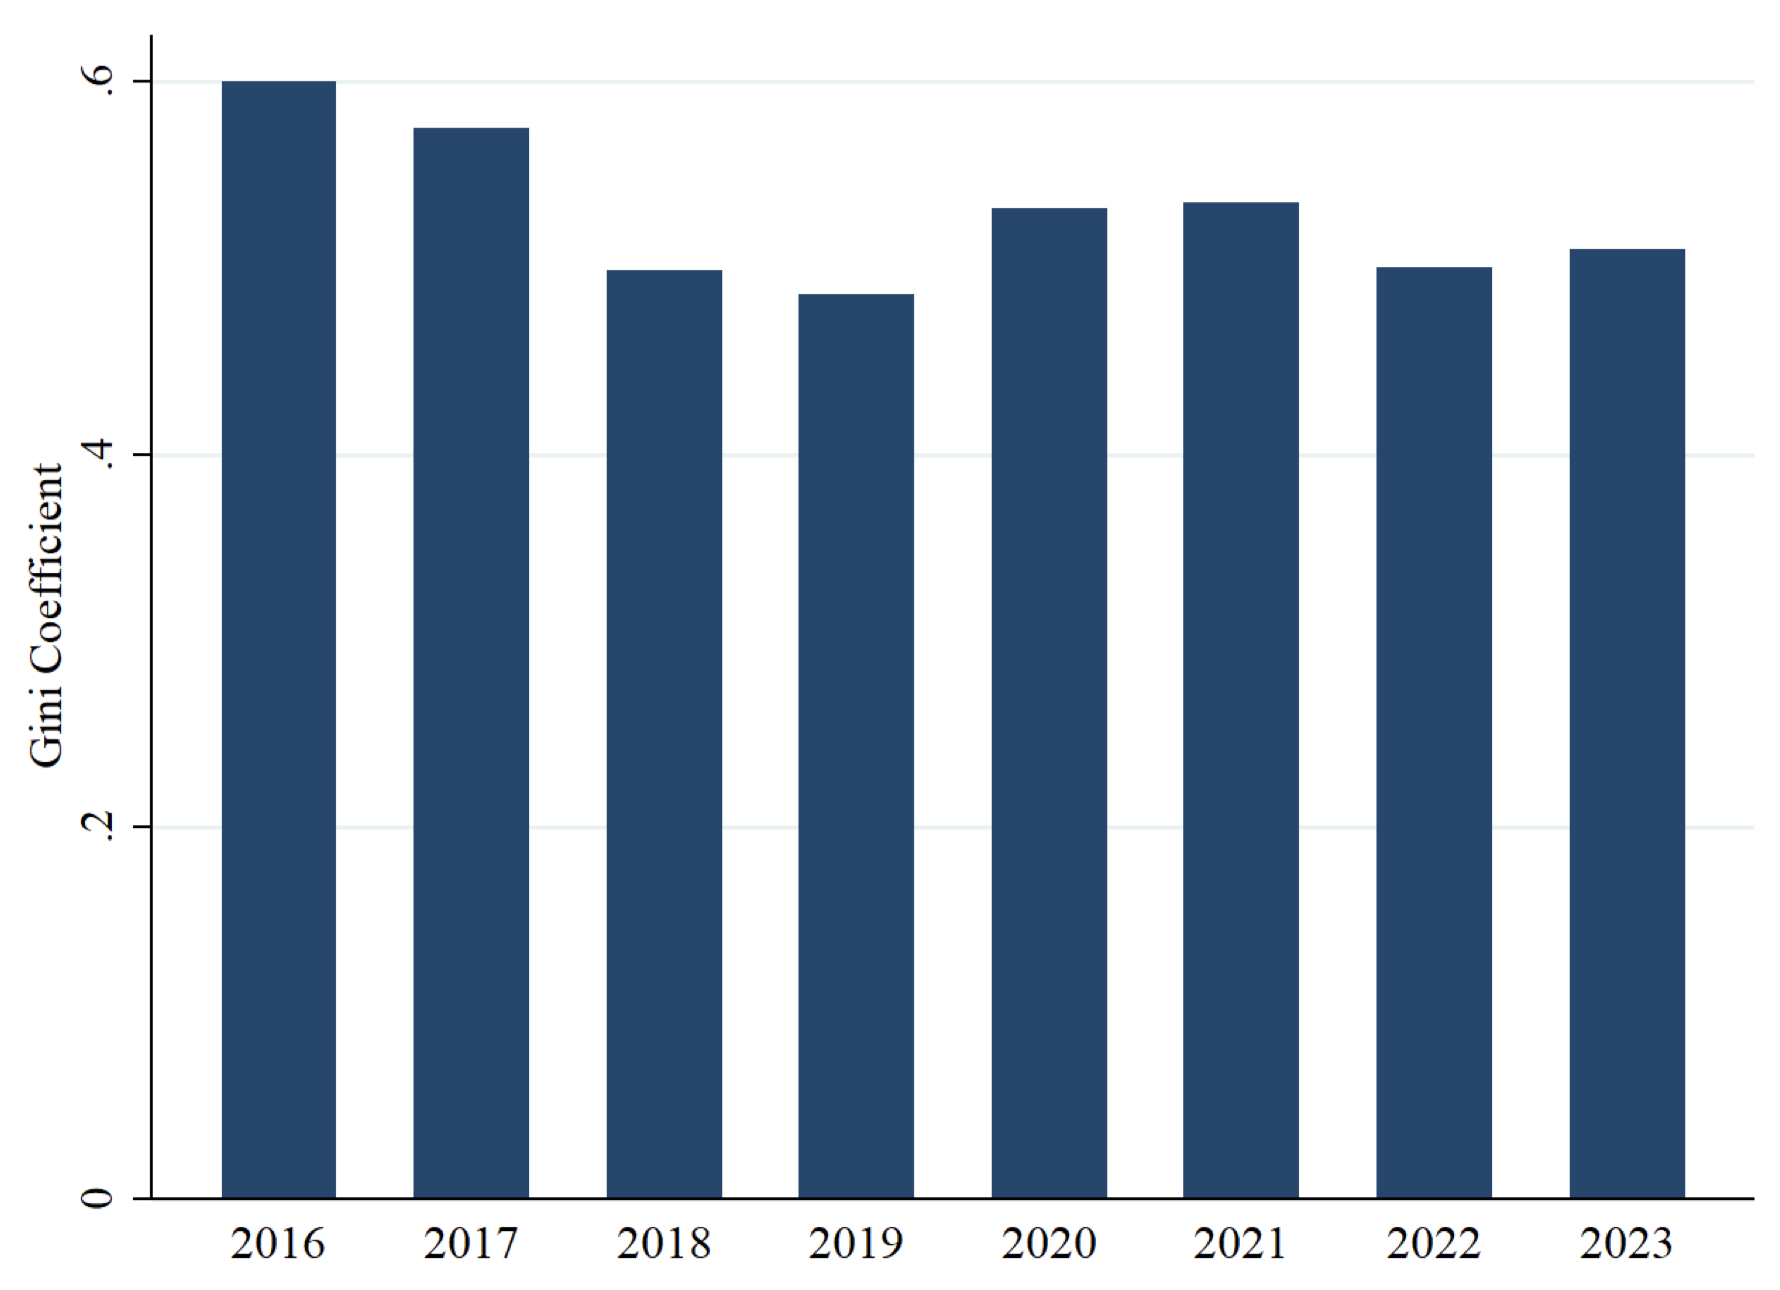
\includegraphics[width=0.85\textwidth]{../Figures/giniEIPConcentration.png}
		\caption{Adapted Gini coefficient for authorship concentration over time.}
	\end{figure}
\end{frame}
%%%


%%%
\begin{frame}[fragile]{EIP Authorship Network}
	\begin{figure}
		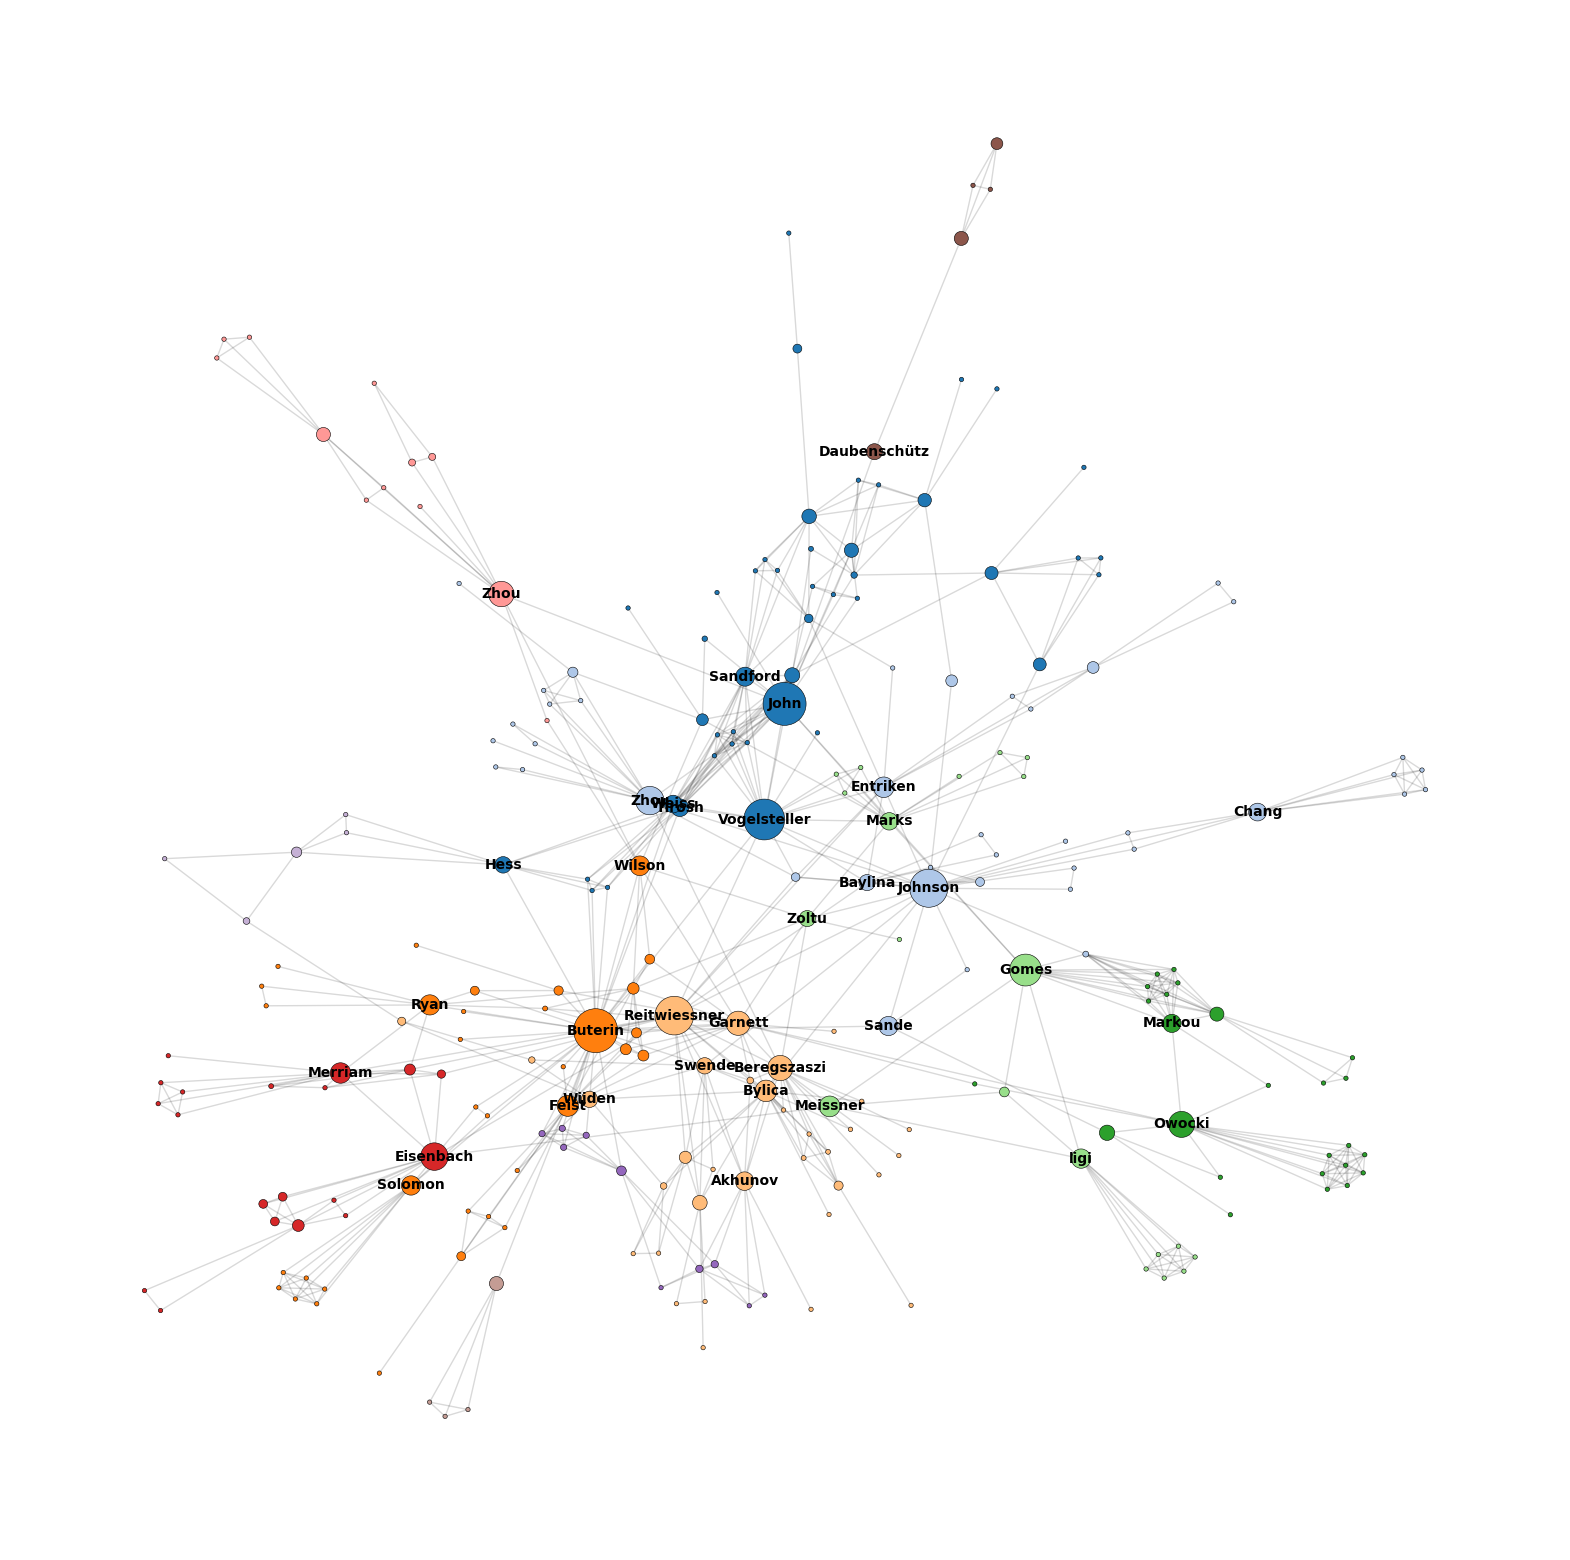
\includegraphics[width = 0.65\textwidth]{../Figures/eip_between_all.png}
        \vspace{-0.9cm}
		\caption{{\small EIP authorship network. The size of each node is proportional to its betweenness centrality value. Names of top 5 percentile of authors displayed, ranked by betweenness centrality.}}
	\end{figure}
\end{frame}
% Betweenness centrality of a node: Number of shortest paths that pass through the node.
% Nodes in the graph are positioned using the Fruchterman-Reingold force-directed algorithm. 
%%%

%%%
\begin{frame}{Average Clustering Coefficient}
	\center
	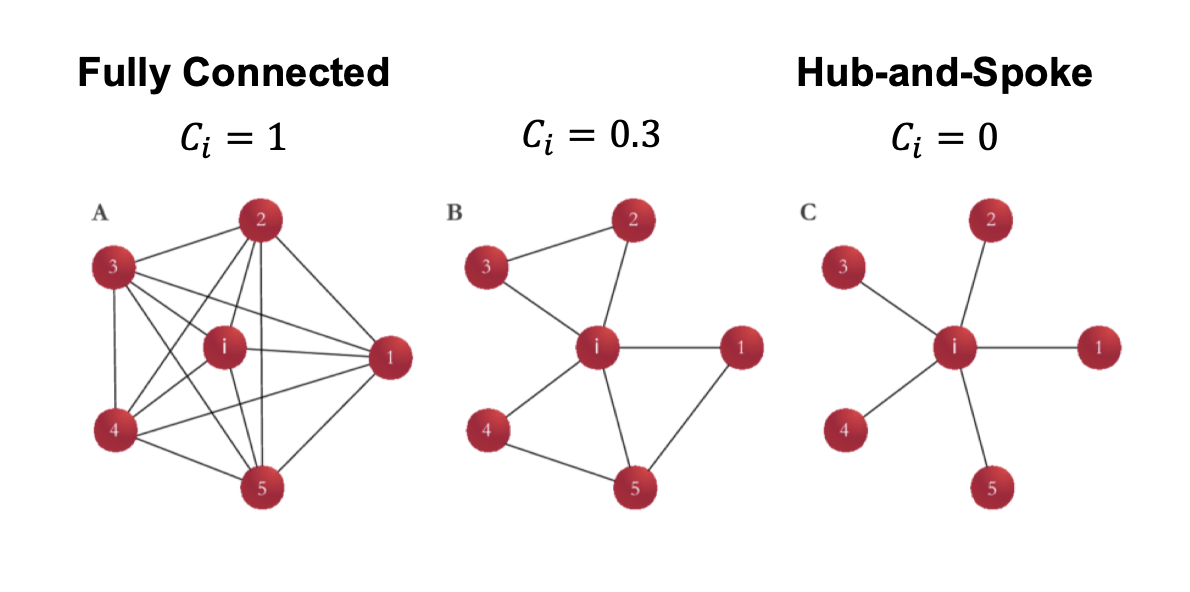
\includegraphics[width=0.8\textwidth]{../Figures/network.png}\\
	\textbf{Intuition:}\\ Number of closed triplets / all triplets (closed and open) 
\end{frame}
%%%
% adjancency matrix
% number of closed triplets divided by number of all triplets.

%%%
\begin{frame}{Clustering Coefficient Over Time}
	\begin{figure}
		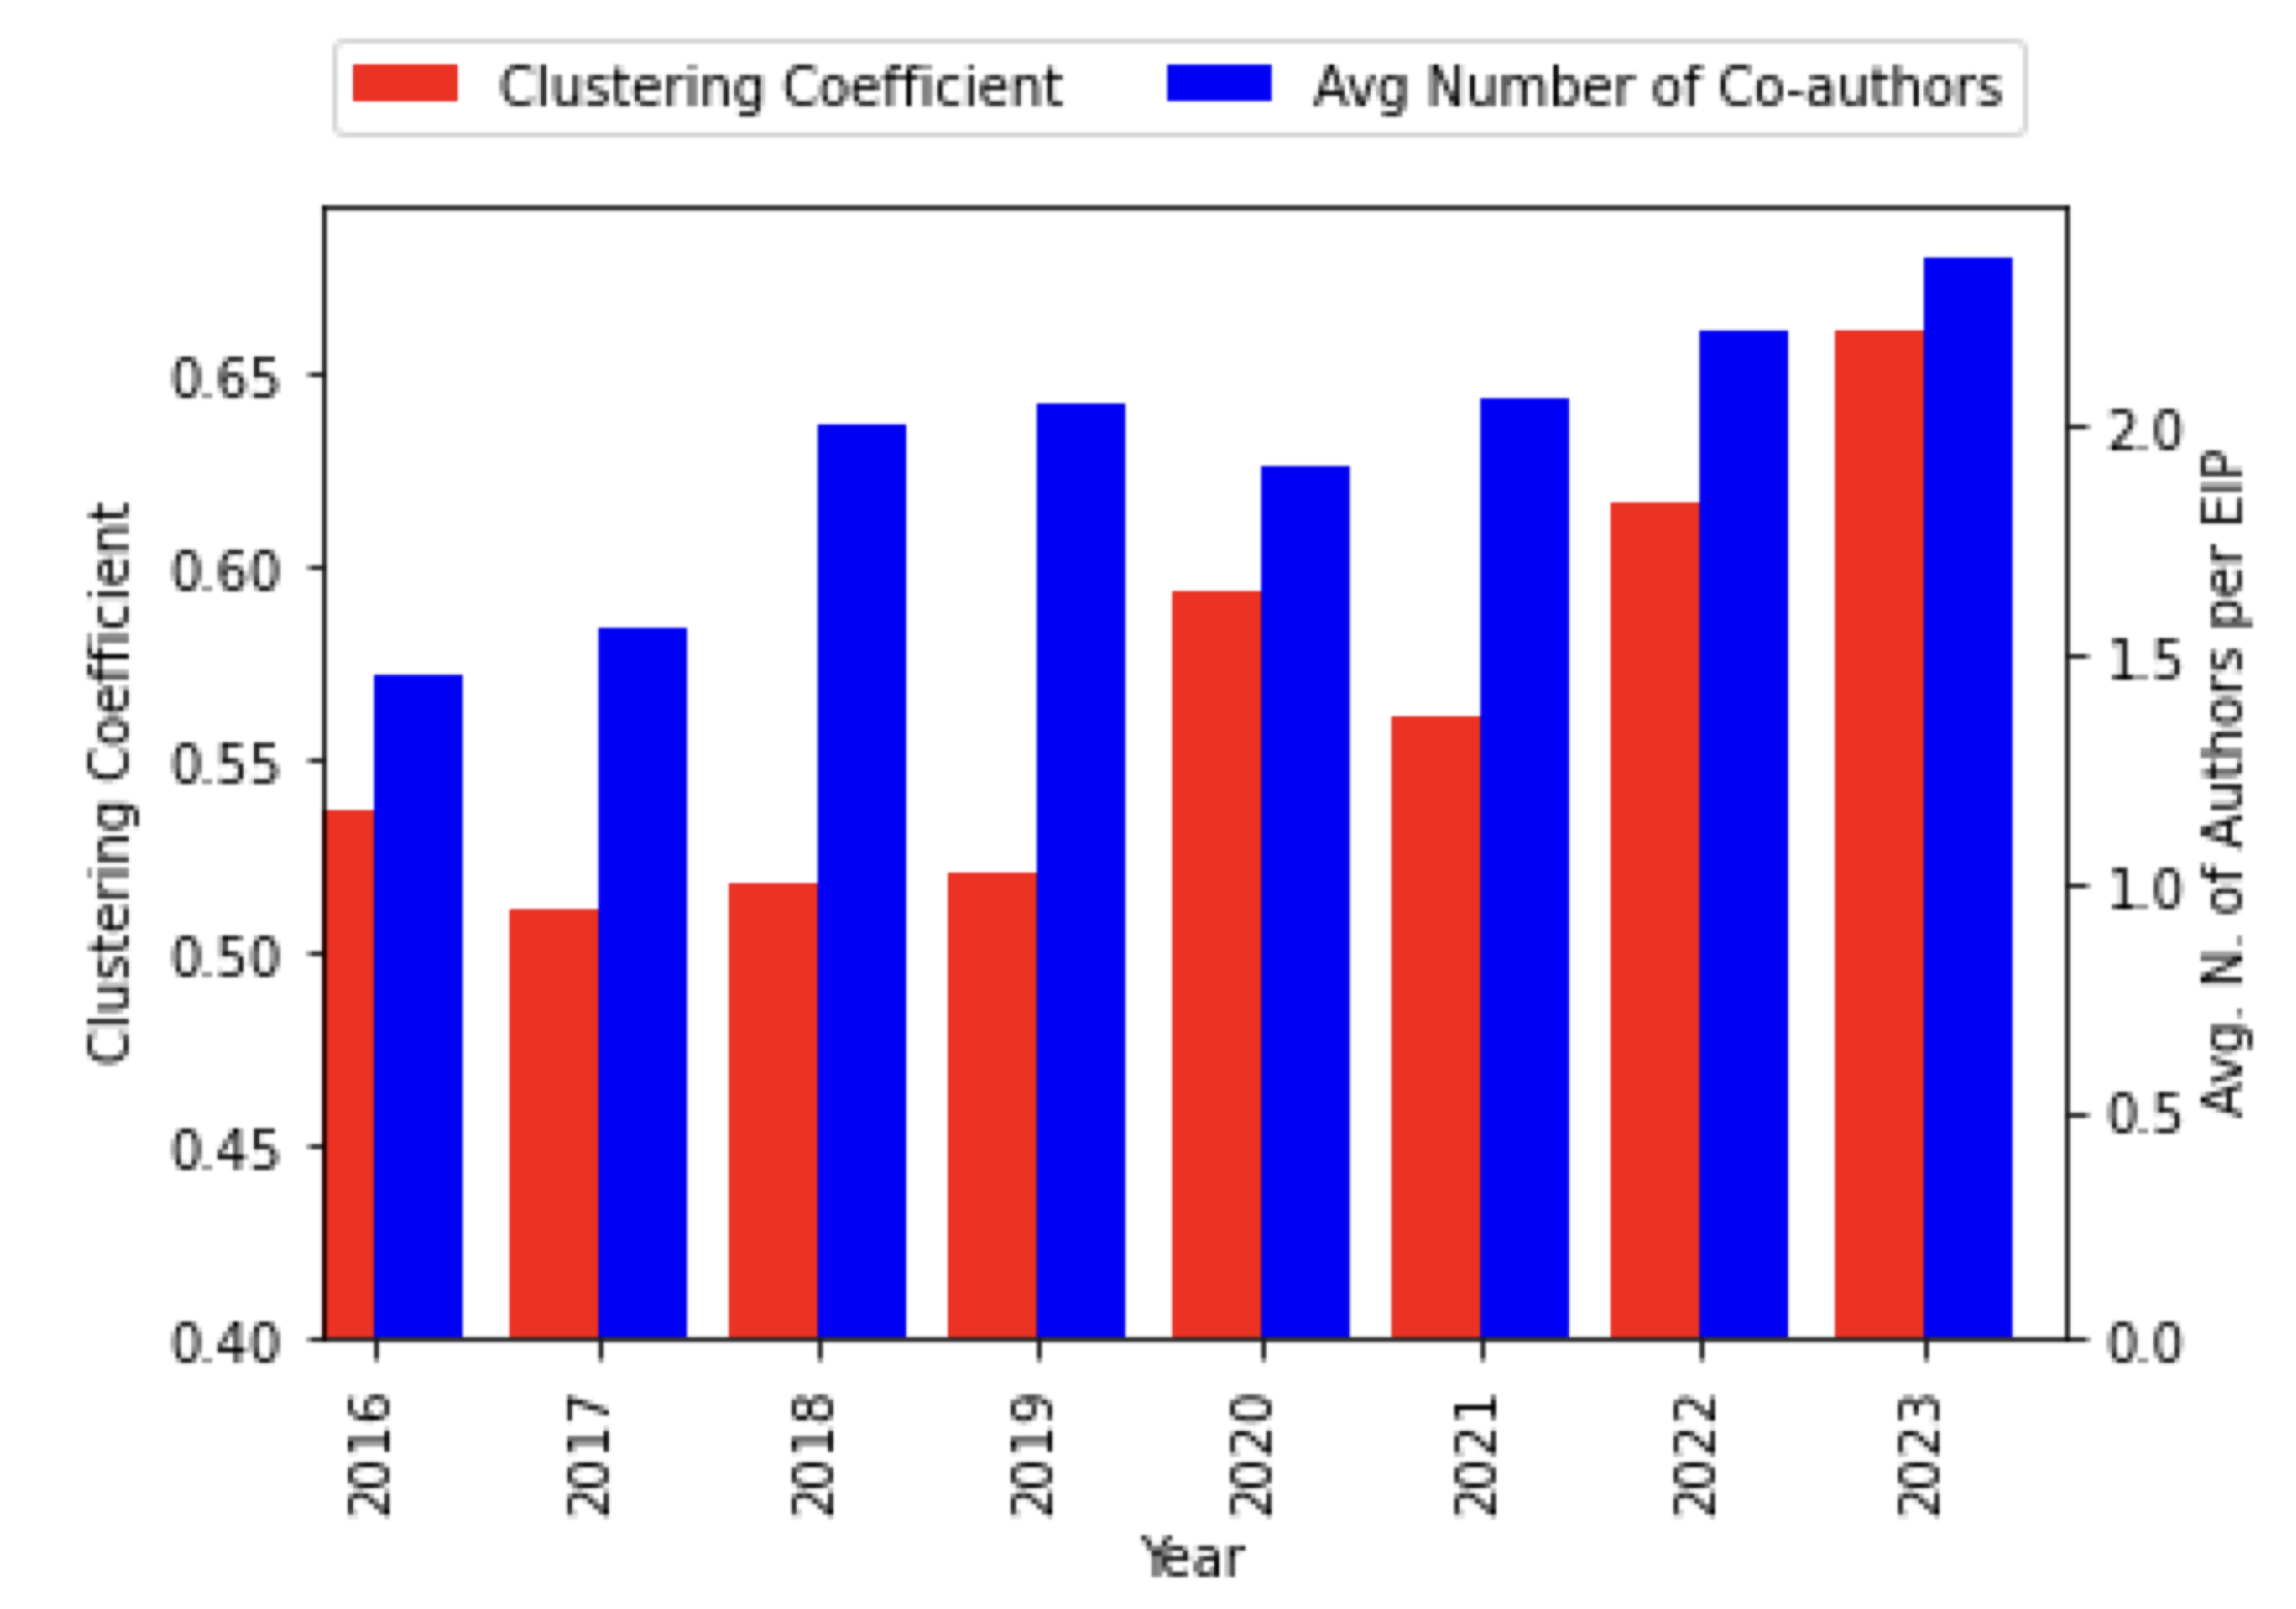
\includegraphics[width = 0.9\textwidth]{../Figures/clusteringDevelopment.png}
        \vspace{-0.6cm}
		\caption{{\small Clustering coefficient and average number of co-authors per EIP over time. Two year rolling window.}}
	\end{figure}
\end{frame}
%%%

%%%%%%%%%%%%%%%%%%%%%%%%%%%%%%%%%%%%%%%%%%%%%
\subsection{Community Engagement}
%%%%%%%%%%%%%%%%%%%%%%%%%%%%%%%%%%%%%%%%%%%%%
%%%
\begin{frame}{Determinants of Community Engagement}
	\begin{table}
		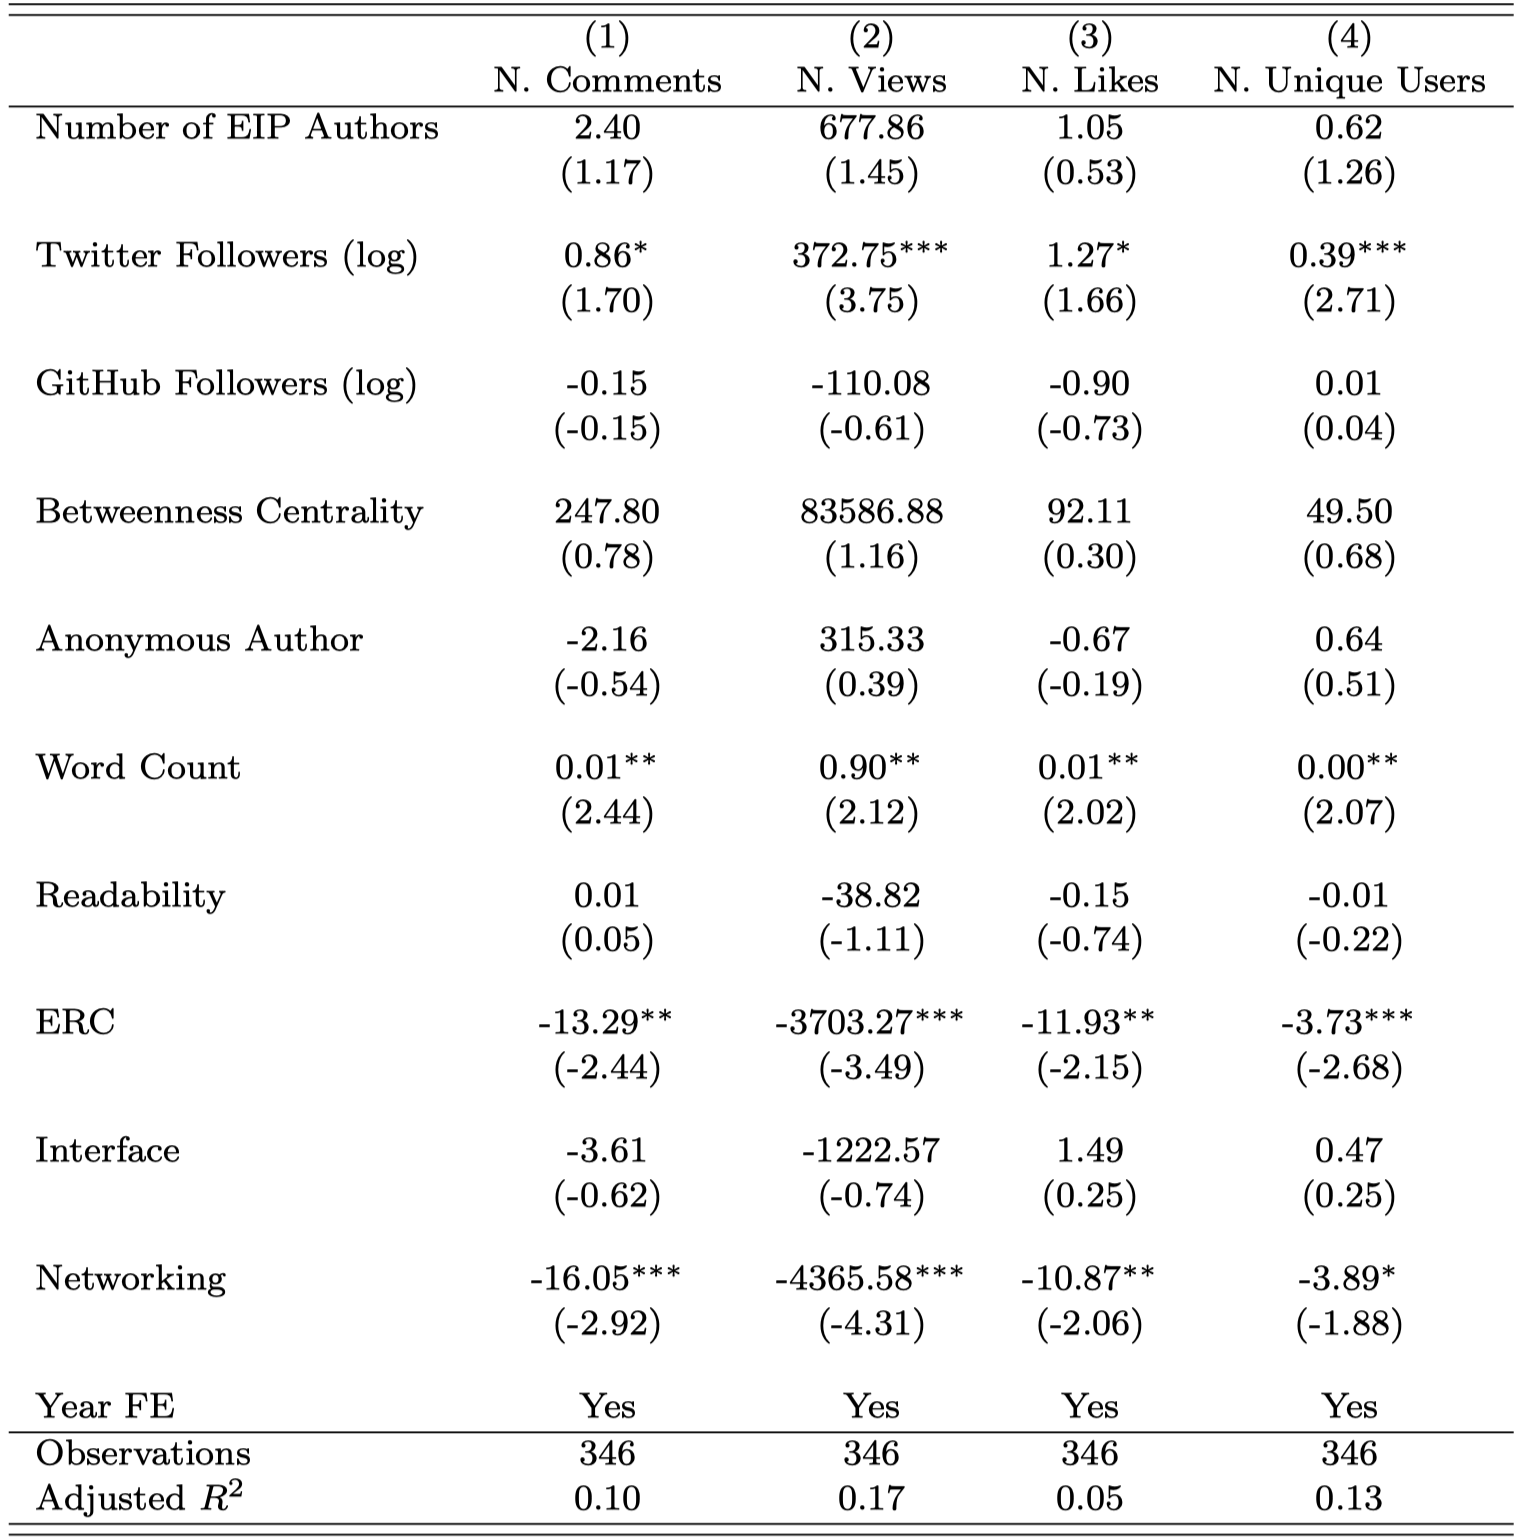
\includegraphics[width=0.7\textwidth]{../Figures/femTable.png}	
		%\caption{}
		
%The table shows the OLS coefficients and t-statistics. Standard errors are adjusted for heteroskedasticity using the Eicker–Huber–White adjustment. Constant is included in all specifications. *, **, and *** indicate statistical significance at the $10\%$, $5\%$, and $1\%$ levels, respectively.   
	\end{table}
\end{frame}
% number of authors
% highest number of github / x followers among co-authors
% author's betweenness centrality
% if at least one of the authors does not display their name
% category dummies -- reference to core.
%%%

\iffalse
%%%
\begin{frame}{EIP Commits around AllCoreDev Calls}
	\begin{figure}
		\includegraphics[width=0.75\textwidth]{../Figures/stackedCohort.png}
		\caption{EIP Github commits around AllCoreDev Meetings. Stacked Cohort Regression Coefficient with 90\% confidence interval. Cohort = AllCoreDevCall. Treatment Group: Discussed EIPs. Control: Other EIPs.}
	\end{figure}
	
	% This figure shows the coefficients of the regression in equation 3. The dotted mark represents the mean of the coefficient, and the line the 90\% confidence interval.
	% We use the agenda of AllCoreDev Meetings
\end{frame}
%%%
\fi

%%%%%%%%%%%%%%%%%%%%%%%%%%%%%%%%%%%%%%%%%%%%%
\subsection{Company/Organization Affiliation}
%%%%%%%%%%%%%%%%%%%%%%%%%%%%%%%%%%%%%%%%%%%%%

%%%
\begin{frame}{EIPs by Author Organization Affiliation}
	\begin{figure}
		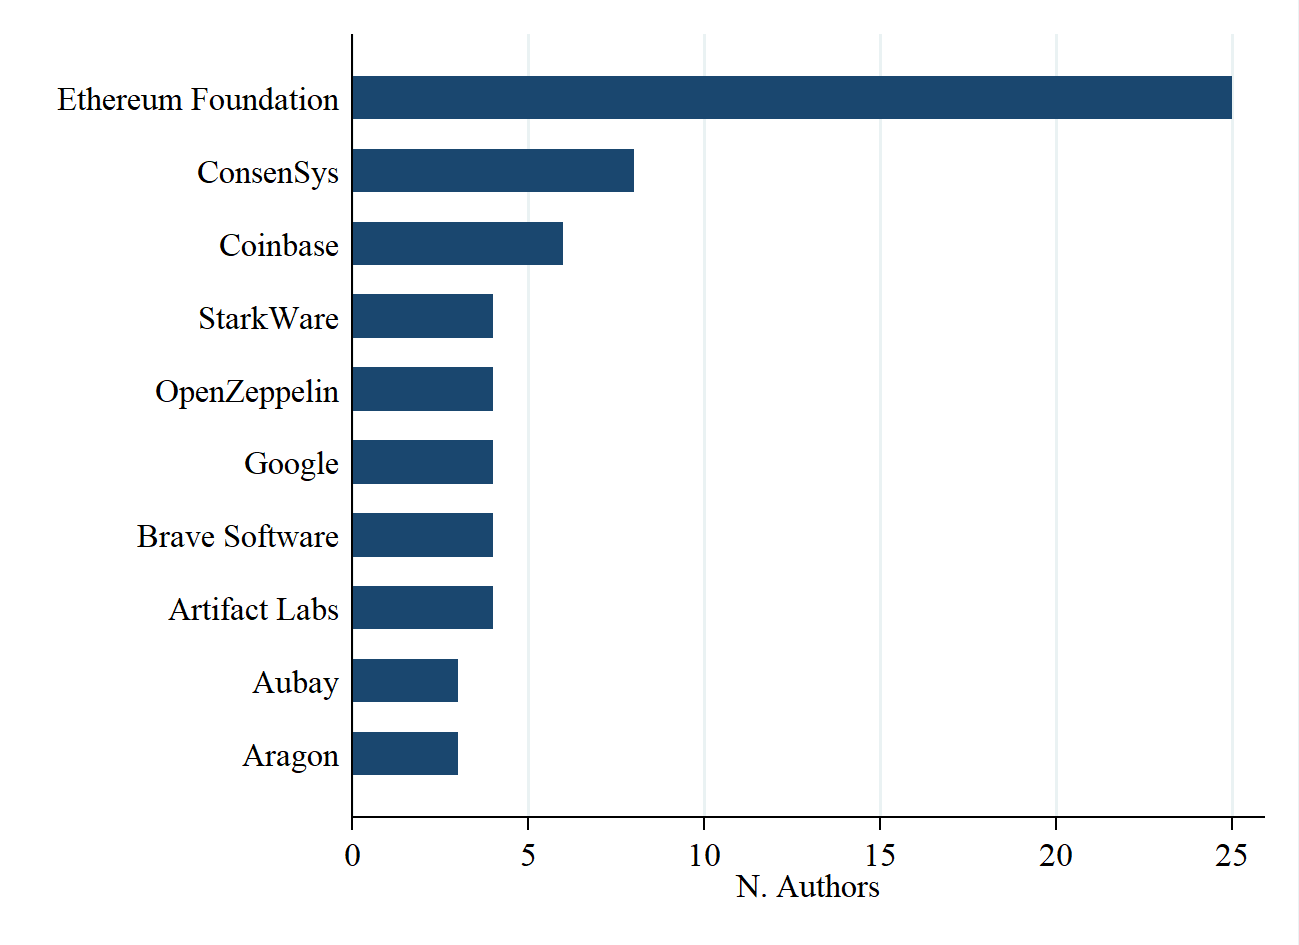
\includegraphics[width= 0.45\textwidth]{../Figures/companyEIP1.png}
		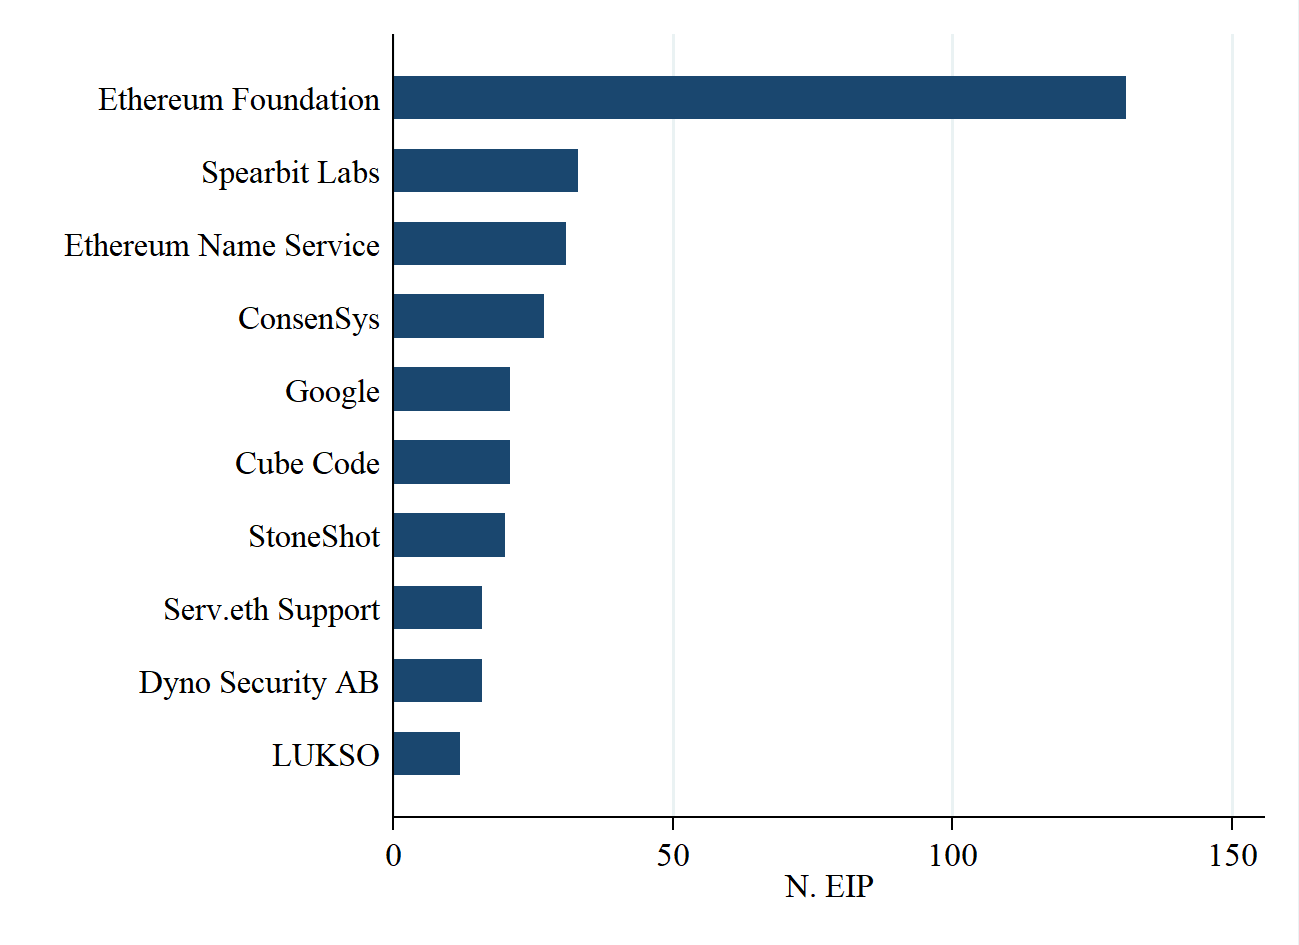
\includegraphics[width= 0.45\textwidth]{../Figures/companyEIP2.png}		
		\caption{Authorship affiliation by number of authors (a) and number of authored EIPs (b).}
	\end{figure}
\end{frame}
%%%
% Swiss foundation, registered in Zug
% 3 directors
% EF sale from July to September 2014
% Approx USD 18 mio in Bitcoin
% Plus premined Ether
% Current on-chain holdings approx. 1 billion USD.


%%%
\begin{frame}{Importance of Ethereum Foundation Over Time}
	\begin{figure}
		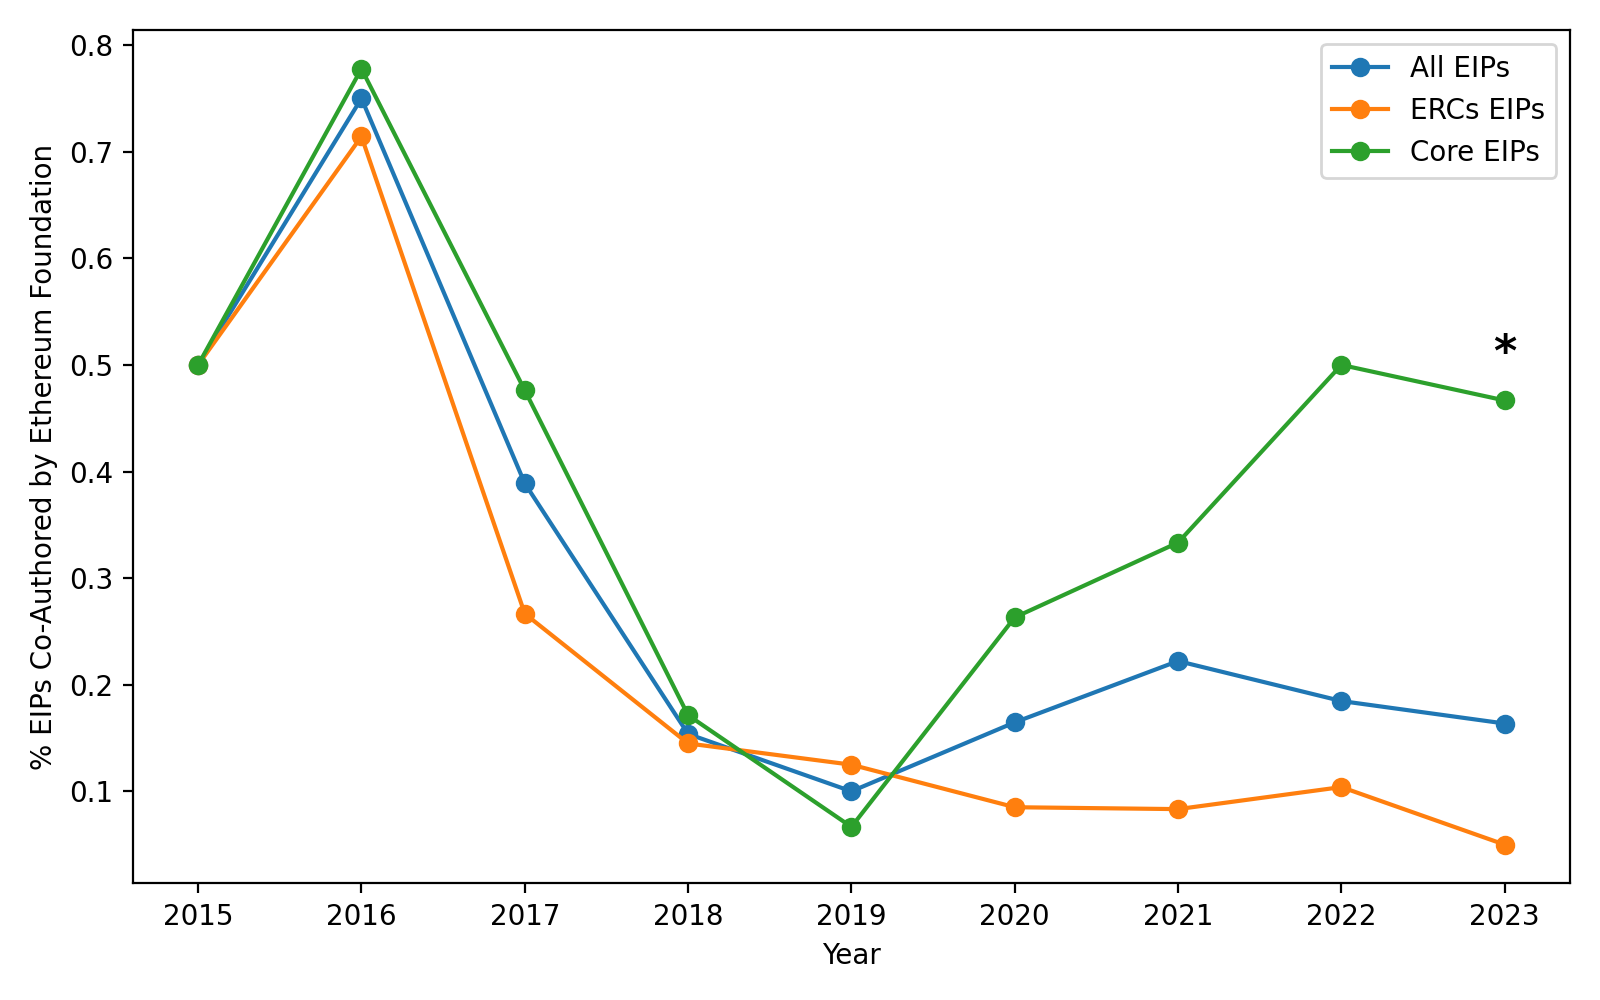
\includegraphics[width= 0.8\textwidth]{../Figures/eip_ef_by_year.png}	
		\caption{Ratio of Ethereum Foundation co-authored EIPs over time.}
	\end{figure}
\end{frame}
%%%



%%%
\iffalse
\begin{frame}\scriptsize
	\begin{table}[ht!]
    \caption{Determinants of Community Engagement}
     \begin{tiny}
    \begin{minipage}{\textwidth}
      The table shows the OLS coefficients and t-statistics. Standard errors are adjusted for heteroskedasticity using the Eicker–Huber–White adjustment. Constant is included in all specifications. *, **, and *** indicate statistical significance at the $10\%$, $5\%$, and $1\%$ levels, respectively.   
  \end{minipage}
    \input{../Tables/FEM_reg_out}
    \label{table:FEM_reg_out}
         \end{tiny}
\end{table}
\end{frame}
\fi
%%%



%%%%%%%%%%%%%%%%%%%%%%%%%%%%%%%%%%%%%%%%%%%%%
\subsection{Effect on Implementation and Adoption}
%%%%%%%%%%%%%%%%%%%%%%%%%%%%%%%%%%%%%%%%%%%%%
%%%
\begin{frame}{EIP Finalization / Implementation}
	\begin{table}
		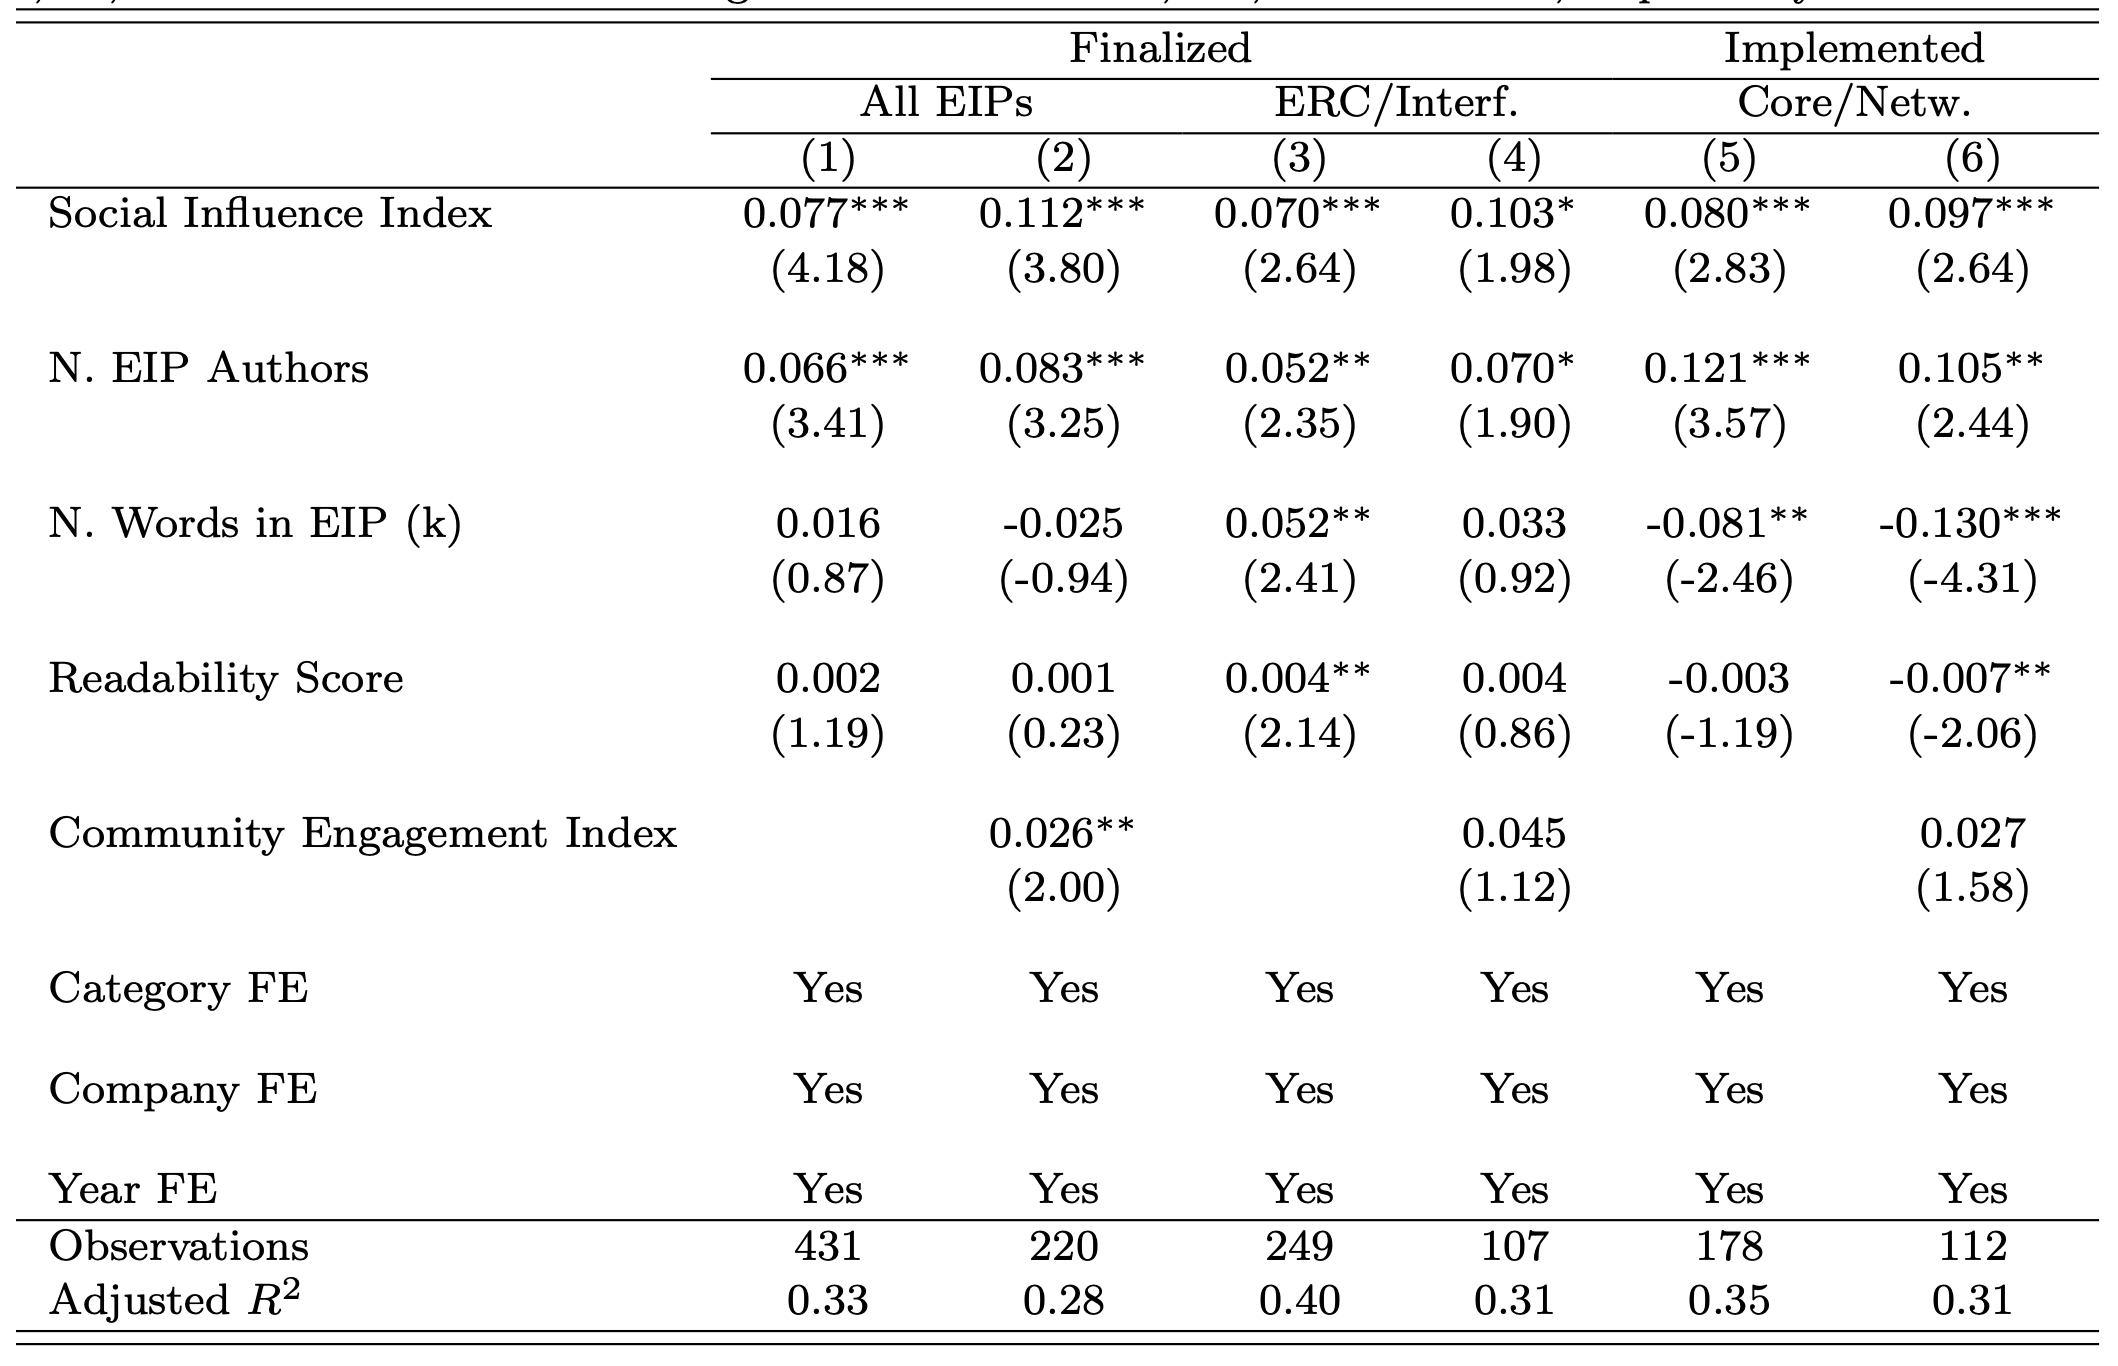
\includegraphics[width= \textwidth]{../Figures/finalizationRegTable.png}
		%\caption{}
	\end{table}
	% The table shows the coefficients and t-statistics of a multivariate OLS regression where the dependent variable is whether an EIP is successfully finalized(columns (1)-(4))/implemented (columns (5)-(6)), or failed (withdrawn or stagnant). In column (1) and (2) we include all EIPs. In columns (3) and (4) we consider only ERC/Interface EIPs, and in columns (5) and (6) only Core/Networking EIPs in columns (1) to (4). We drop EIPs that are in progress (Draft, Review, Lat Call). Standard errors are adjusted for heteroskedasticity using the Eicker–Huber–White adjustment. Constant is included in all specifications. *, **, and *** indicate statistical significance at the 10%, 5%, and 1% levels, respectively.
\end{frame}
% Social Influence index: highest number of github and x followers among co-authors, highest betweenness centrality, and whether one of the co-authors chooses to remain anonymous. -> First component of a PCA.
% Community Engagement: comments, views, likes and users on Fellowship of Ethereum Magicians.
% A one standard deviation increase (1.5) in the authors’ social influence is associated with a EIPs have a 12%-17% higher chance of being finalized. Similarly, the community engagement is a strong predictor of EIP finalization.
% a one standard deviation increase in engagement (1.9) is associated with a 5% more likelihood of success.
%%%

%%%
\begin{frame}{Company Effects (Top 10)}
	\begin{figure}
		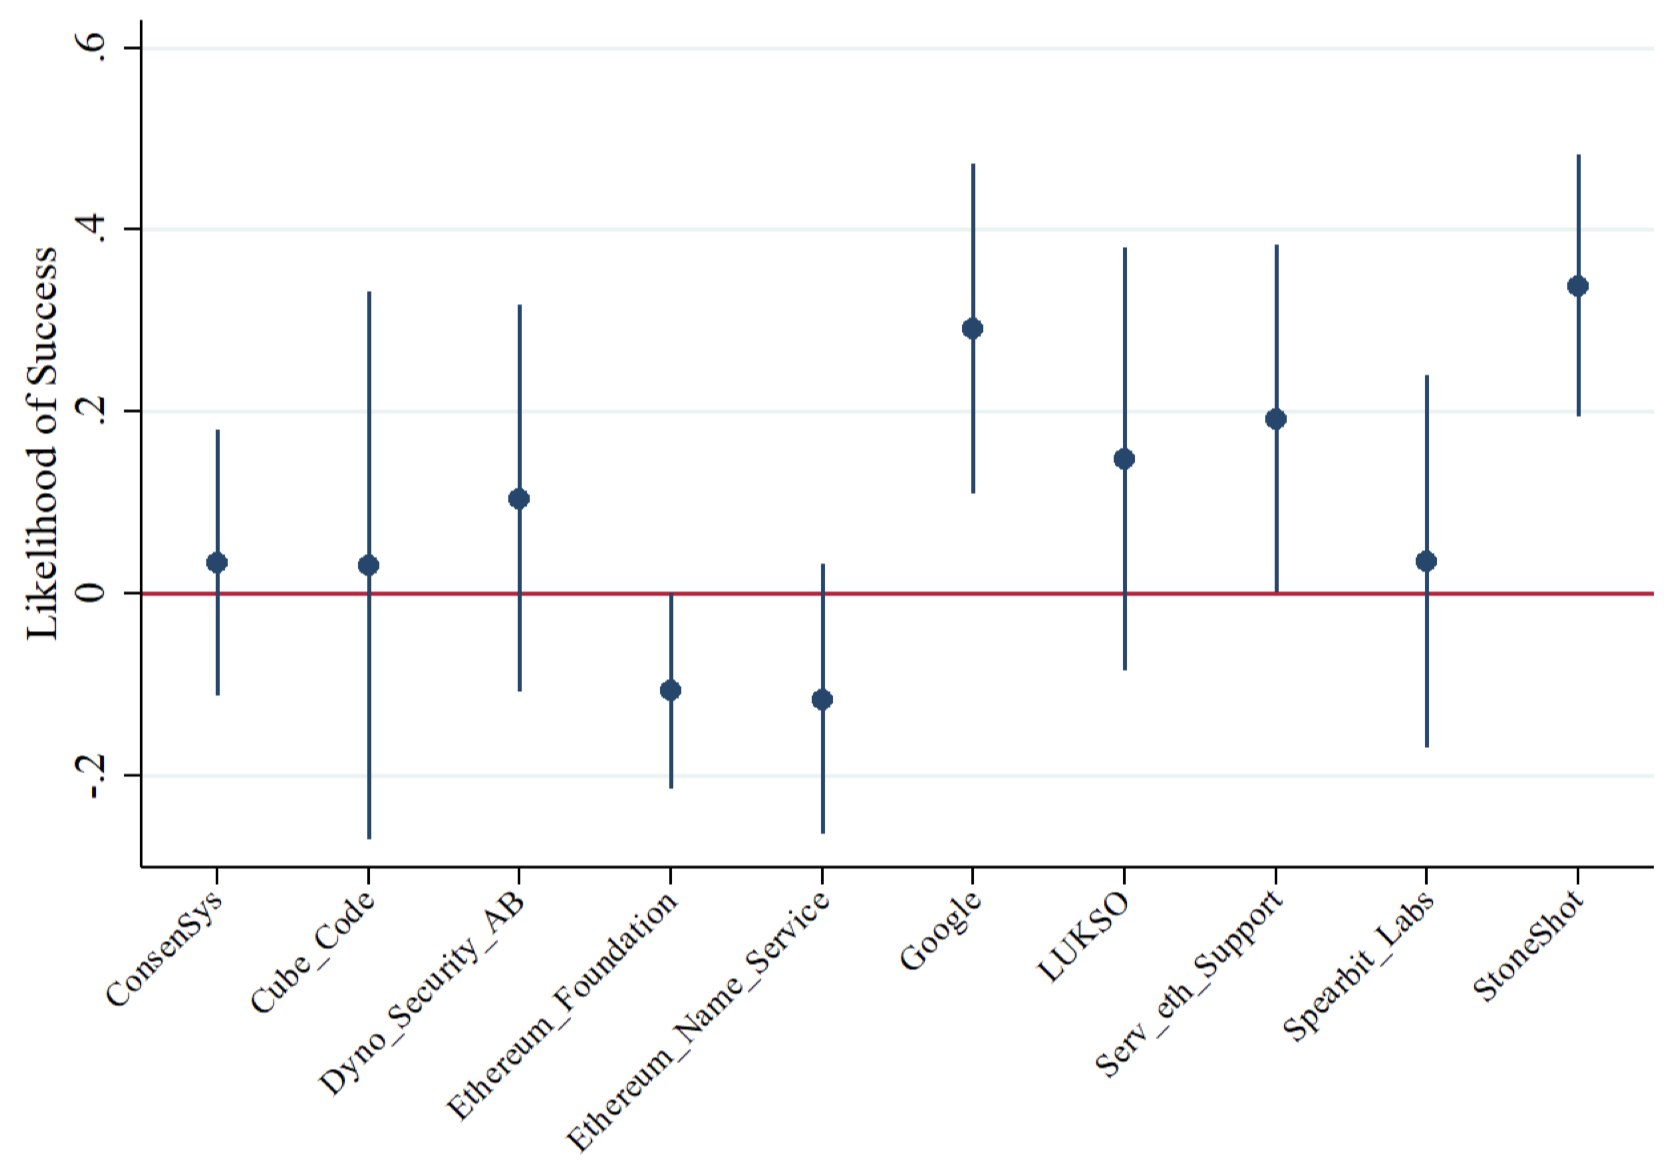
\includegraphics[width= 0.9\textwidth]{../Figures/companyEffects.png}
		\caption{Company fixed effects. Regression coefficients and 0.9 confidence interval. F-value of 3.44 and a p-value of 0.0002.}
	\end{figure}
\end{frame}
%%%


%%%%%%%%%%%%%%%%%%%%%%%%%%%%%%%%%%%%%%%%%%%%%
\subsection{Client Development Concentration}
%%%%%%%%%%%%%%%%%%%%%%%%%%%%%%%%%%%%%%%%%%%%%

%%%
\begin{frame}{The Ethereum Protocol Stack}

Clients are software applications that process and exchange information in accordance with the Ethereum protocol (essentially a processing and communication standard). A \textit{full node} consists of an \textit{execution client} and a \textit{consensus client}, usually running on the same computer. \vspace{0.8em}

    \begin{columns}
        % Column 1
        \begin{column}{0.5\textwidth}
            % Content of the first column
            \textbf{Execution Clients}\\
            \begin{itemize}
                \item Go-Ethereum ($\sim$52\%)
                \item Nethermind ($\sim$30\%)
                \item Besu ($\sim$15\%)
                \item Erigon ($\sim$2\%)
                \item Reth ($\sim$1\%)
                \item ...
            \end{itemize}
        \end{column}
        
        % Column 2
        \begin{column}{0.5\textwidth}
            % Content of the second column
            \textbf{Consensus Clients}\\
            \begin{itemize}
                \item Prysm ($\sim$37\%)
                \item Lighthouse ($\sim$33\%)
                \item Teku ($\sim$21\%)
                \item Nimbus ($\sim$9\%)
                \item Lodestar ($\sim$0\%)
                \item ...
                %\item Grandine
            \end{itemize}
        \end{column}    
    \end{columns} \vfill
    
    \tiny{Data Source: \url{clientdiversity.org} via Sonic (Execution) and Blockprint (Consensus). Snapshot October 18th, 2024.}

\end{frame}
%%%

%%%
\begin{frame}{Role Overlap}
	\begin{figure}
		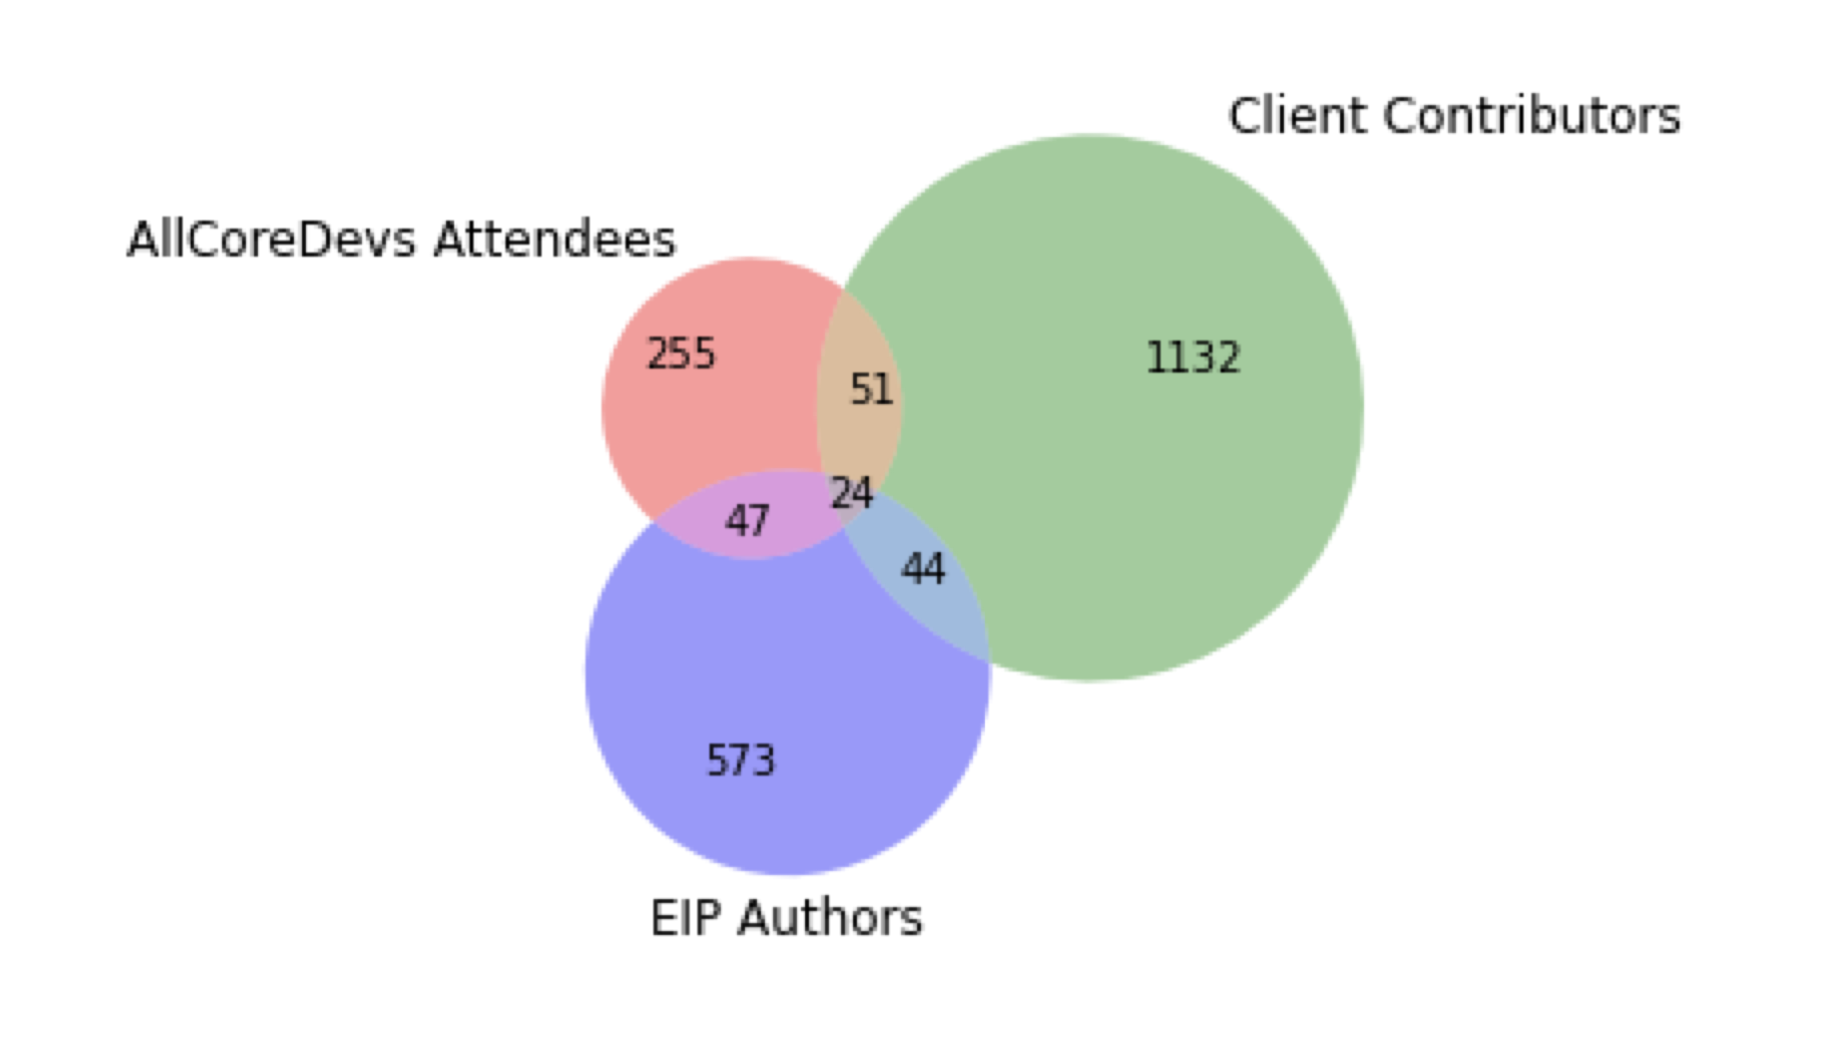
\includegraphics[width = \textwidth]{../Figures/contributorsOverlap.png}
		\caption{Overlap of important contributor roles.}
	\end{figure}
\end{frame}
% 75% of contributors have fewer than 7 commits. 
%%%

%%%
\begin{frame}{Client Commits}
	\begin{figure}
		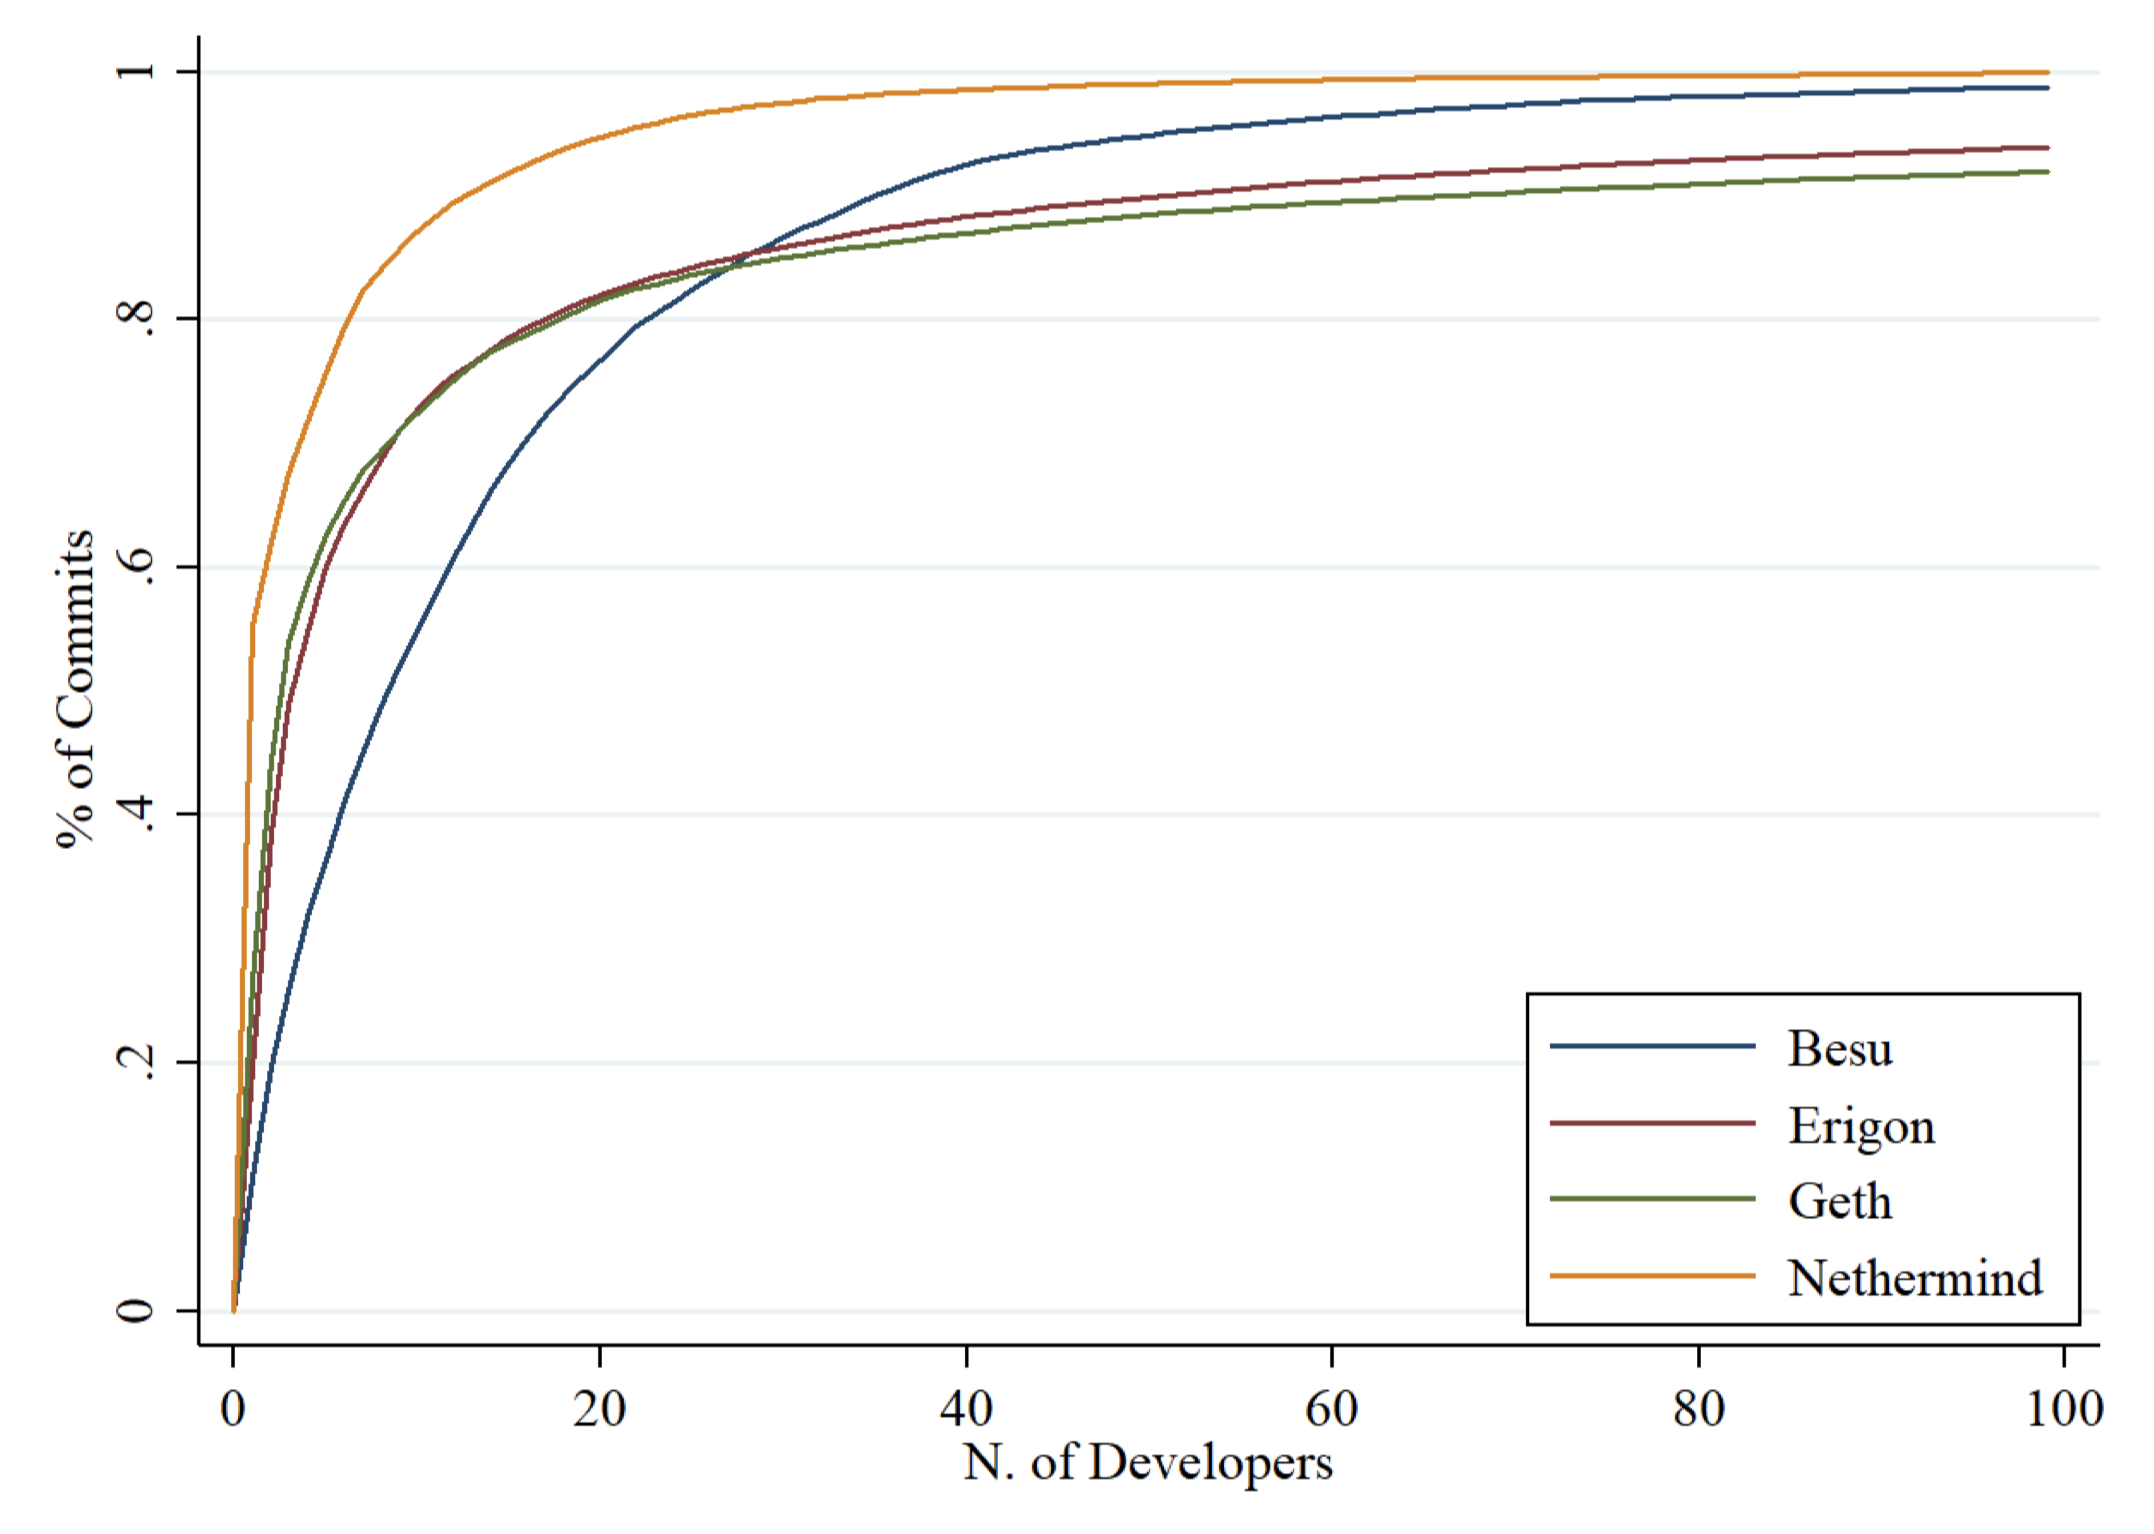
\includegraphics[width = 0.9\textwidth]{../Figures/clientCommits.png}
		\caption{Lorenz curve adapted to client commit concentration.}
	\end{figure}
\end{frame}
% For all clients 20 or less developers who are responsible or 80% of the commits
%%%

%%%
\begin{frame}{Execution Client Developer Affiliation}
	\begin{figure}
		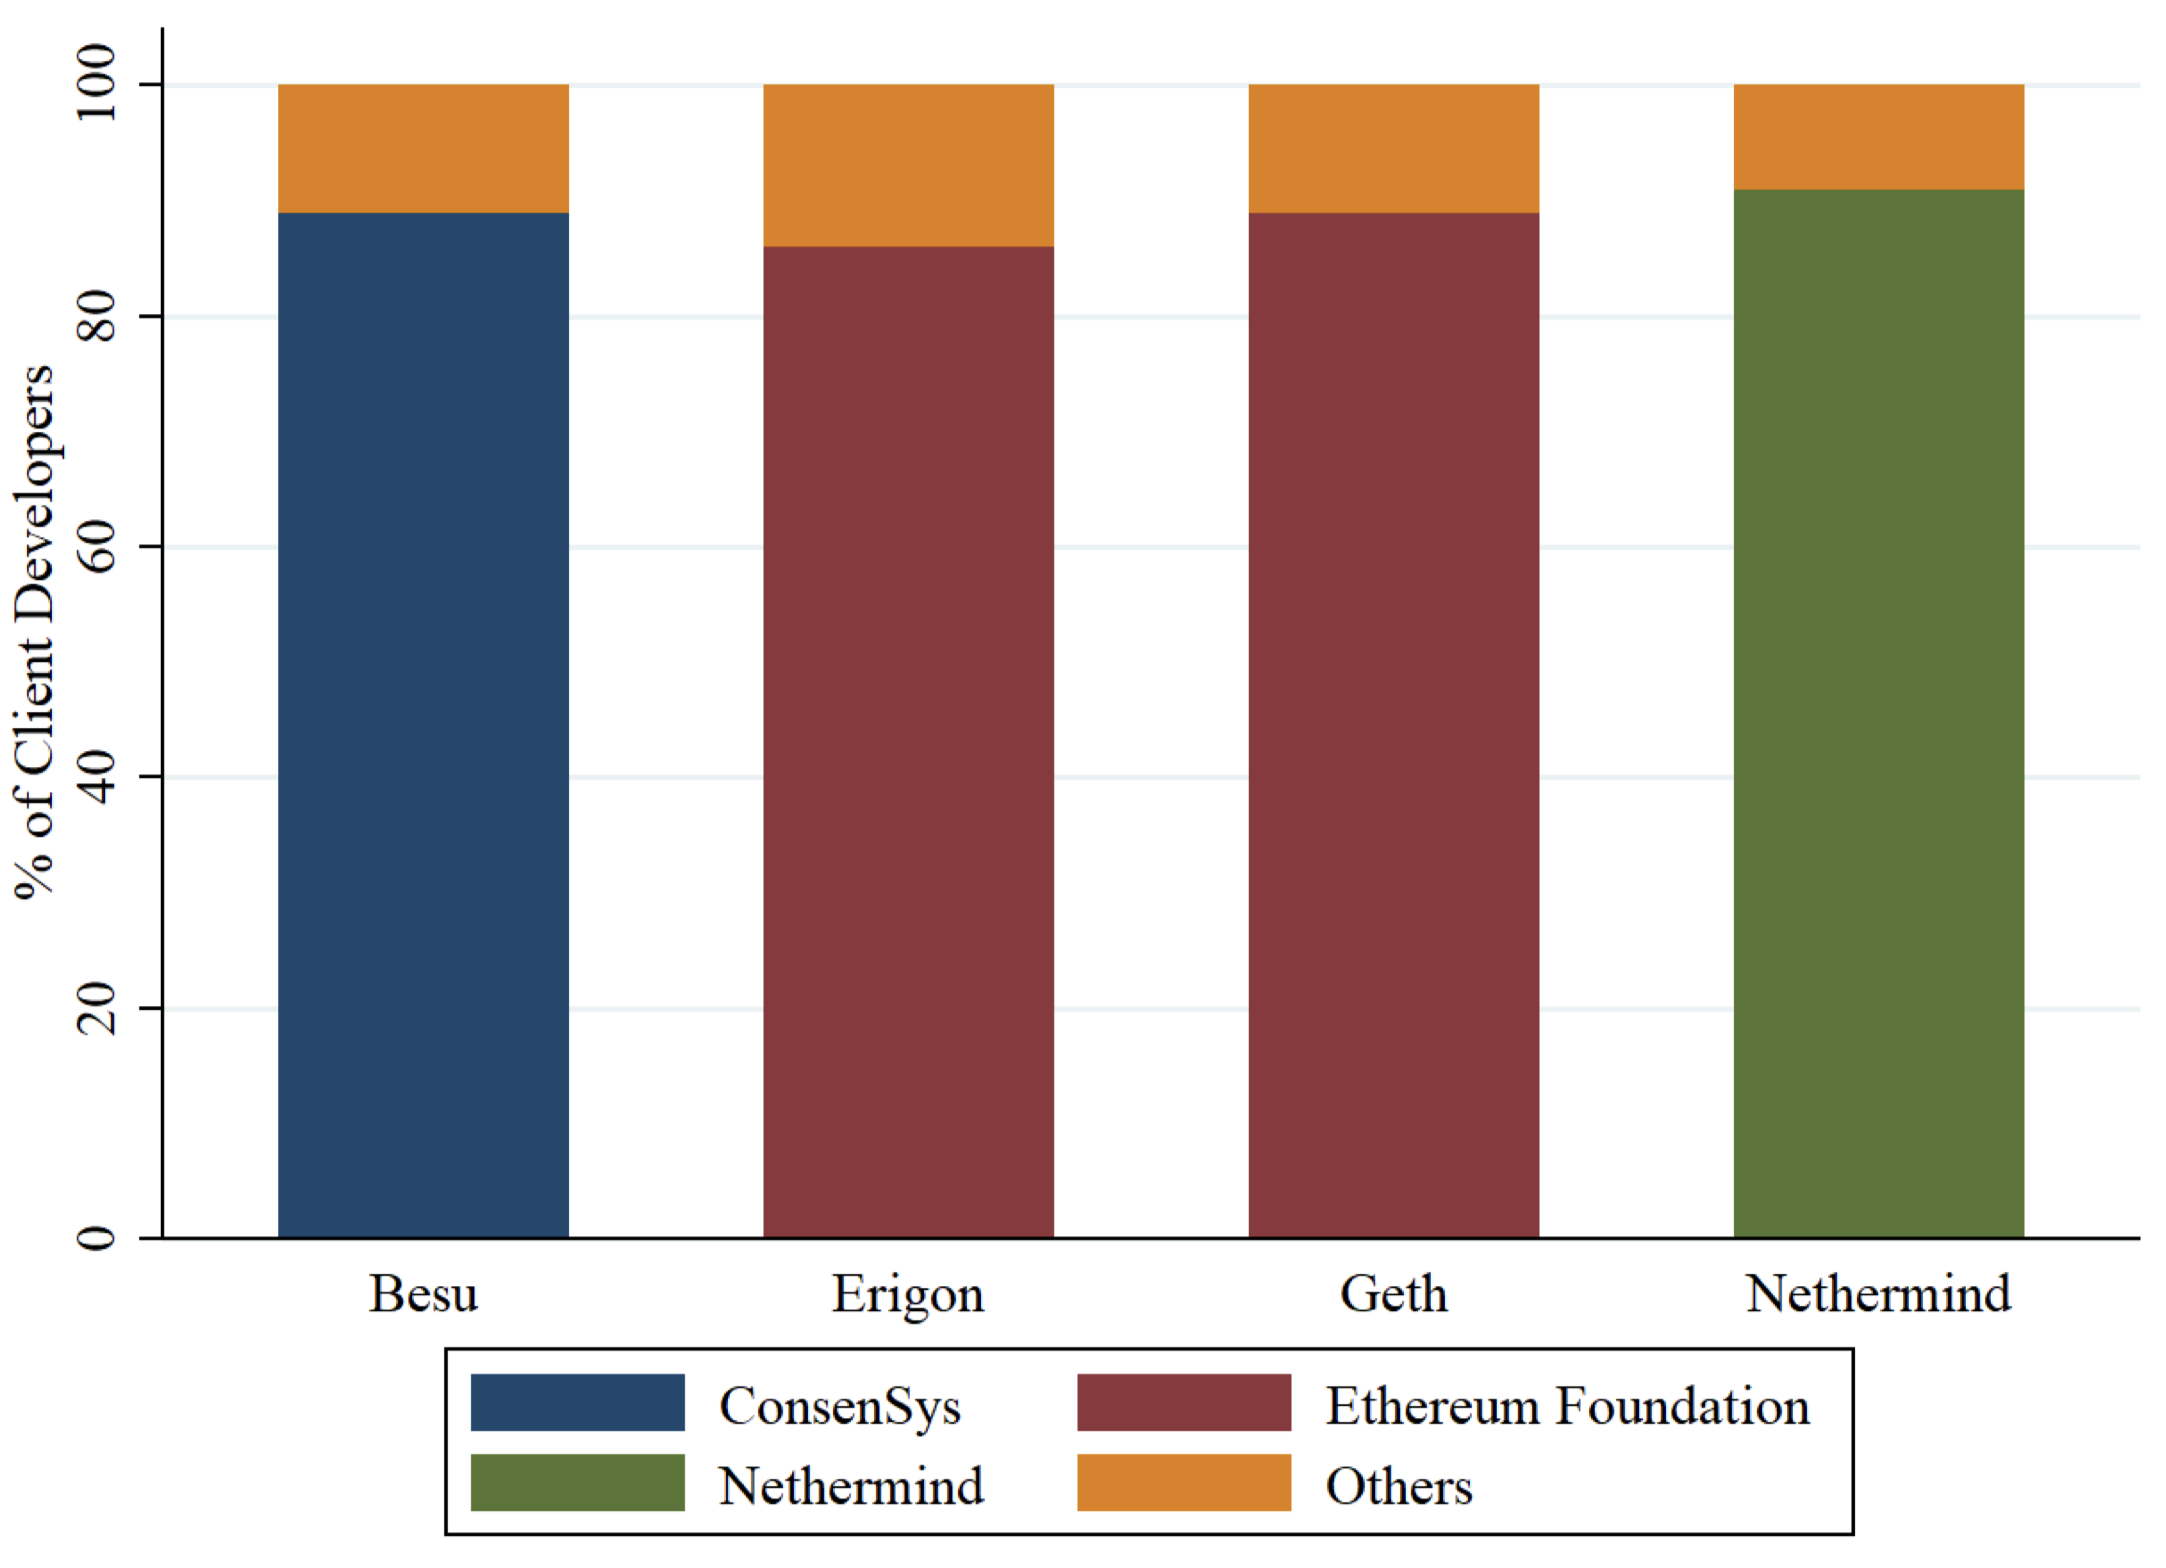
\includegraphics[width = 0.85\textwidth]{../Figures/clientDevs.png}
		\caption{Execution Clients by top-20 dev affiliation.}
	\end{figure}
\end{frame}
%%%


%%%%%%%%%%%%%%%%%%%%%%%%%%%%%%%%%%%%%%%%%%%%%
\subsection{Reverse Dependencies}
%%%%%%%%%%%%%%%%%%%%%%%%%%%%%%%%%%%%%%%%%%%%%
%%%
\begin{frame}{Reverse Dependencies}
	\begin{figure}
		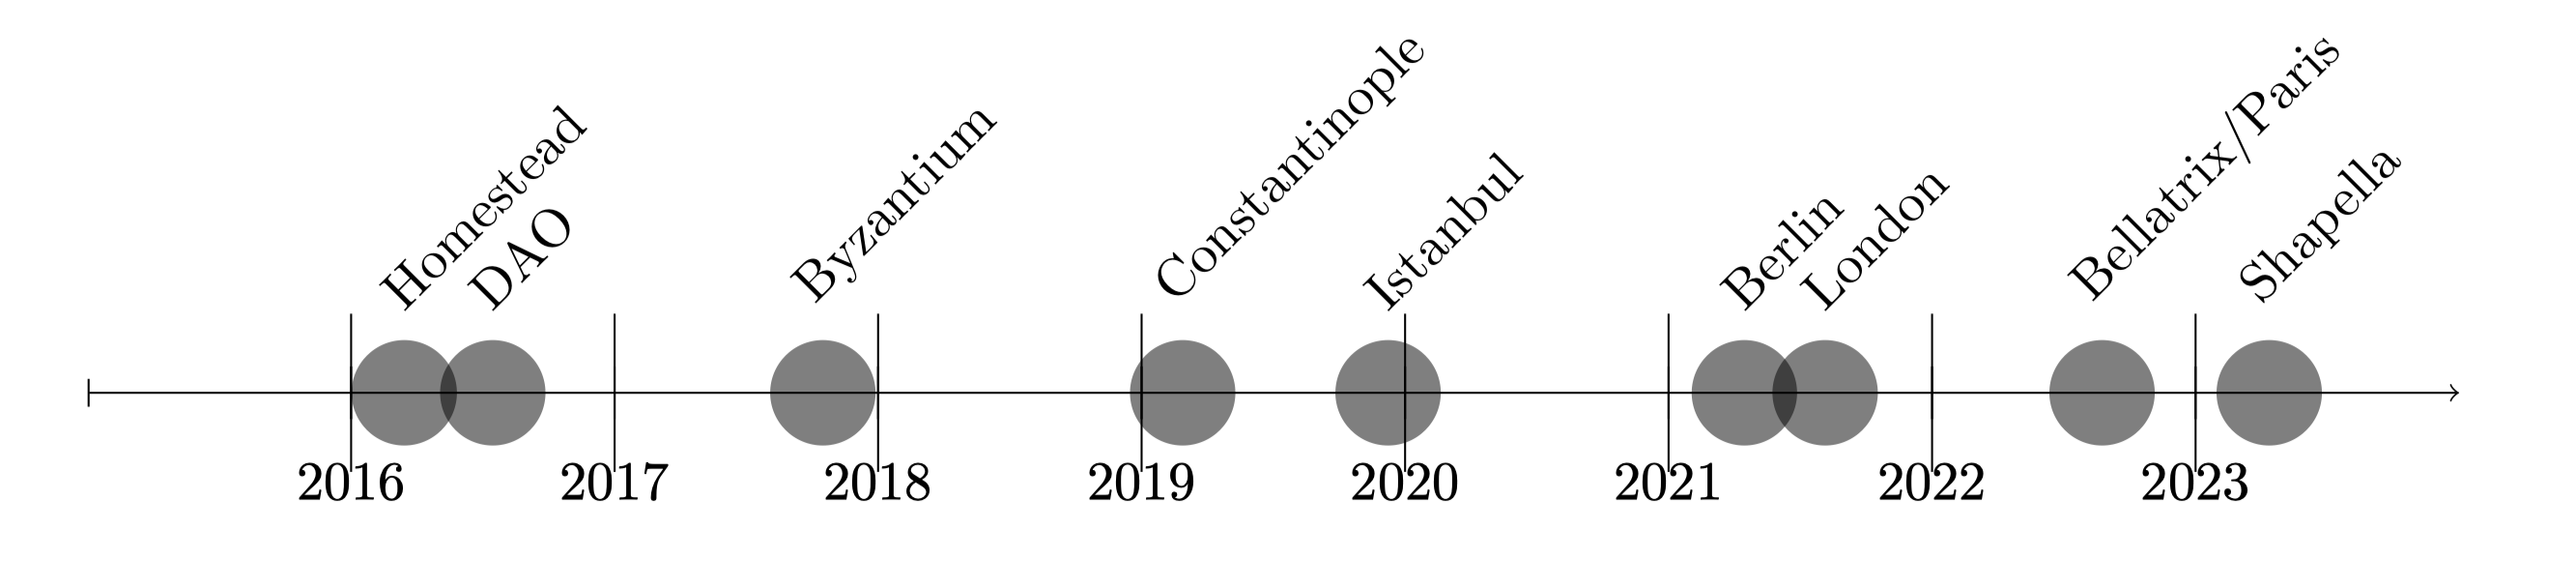
\includegraphics[width = \textwidth]{../Figures/forkHistory.png}
		\caption{Timeline of major Ethereum Forks.}
	\end{figure}
	
	\vspace{-0.5cm}
	\textbf{In case of a disagreement:}
	\begin{itemize}
		\item Network splits lead to multiple co-existing versions of the blockchain. 
		\item Off-chain collateralized assets will only work on one version (e.g., stablecoins).
		\item Protocols with off-chain dependencies may not be supported on all chains (e.g., oracles).
	\end{itemize}
	
\end{frame}
%%%

%%%
\begin{frame}{Stablecoin Collateral Market Share}
		\begin{figure}
		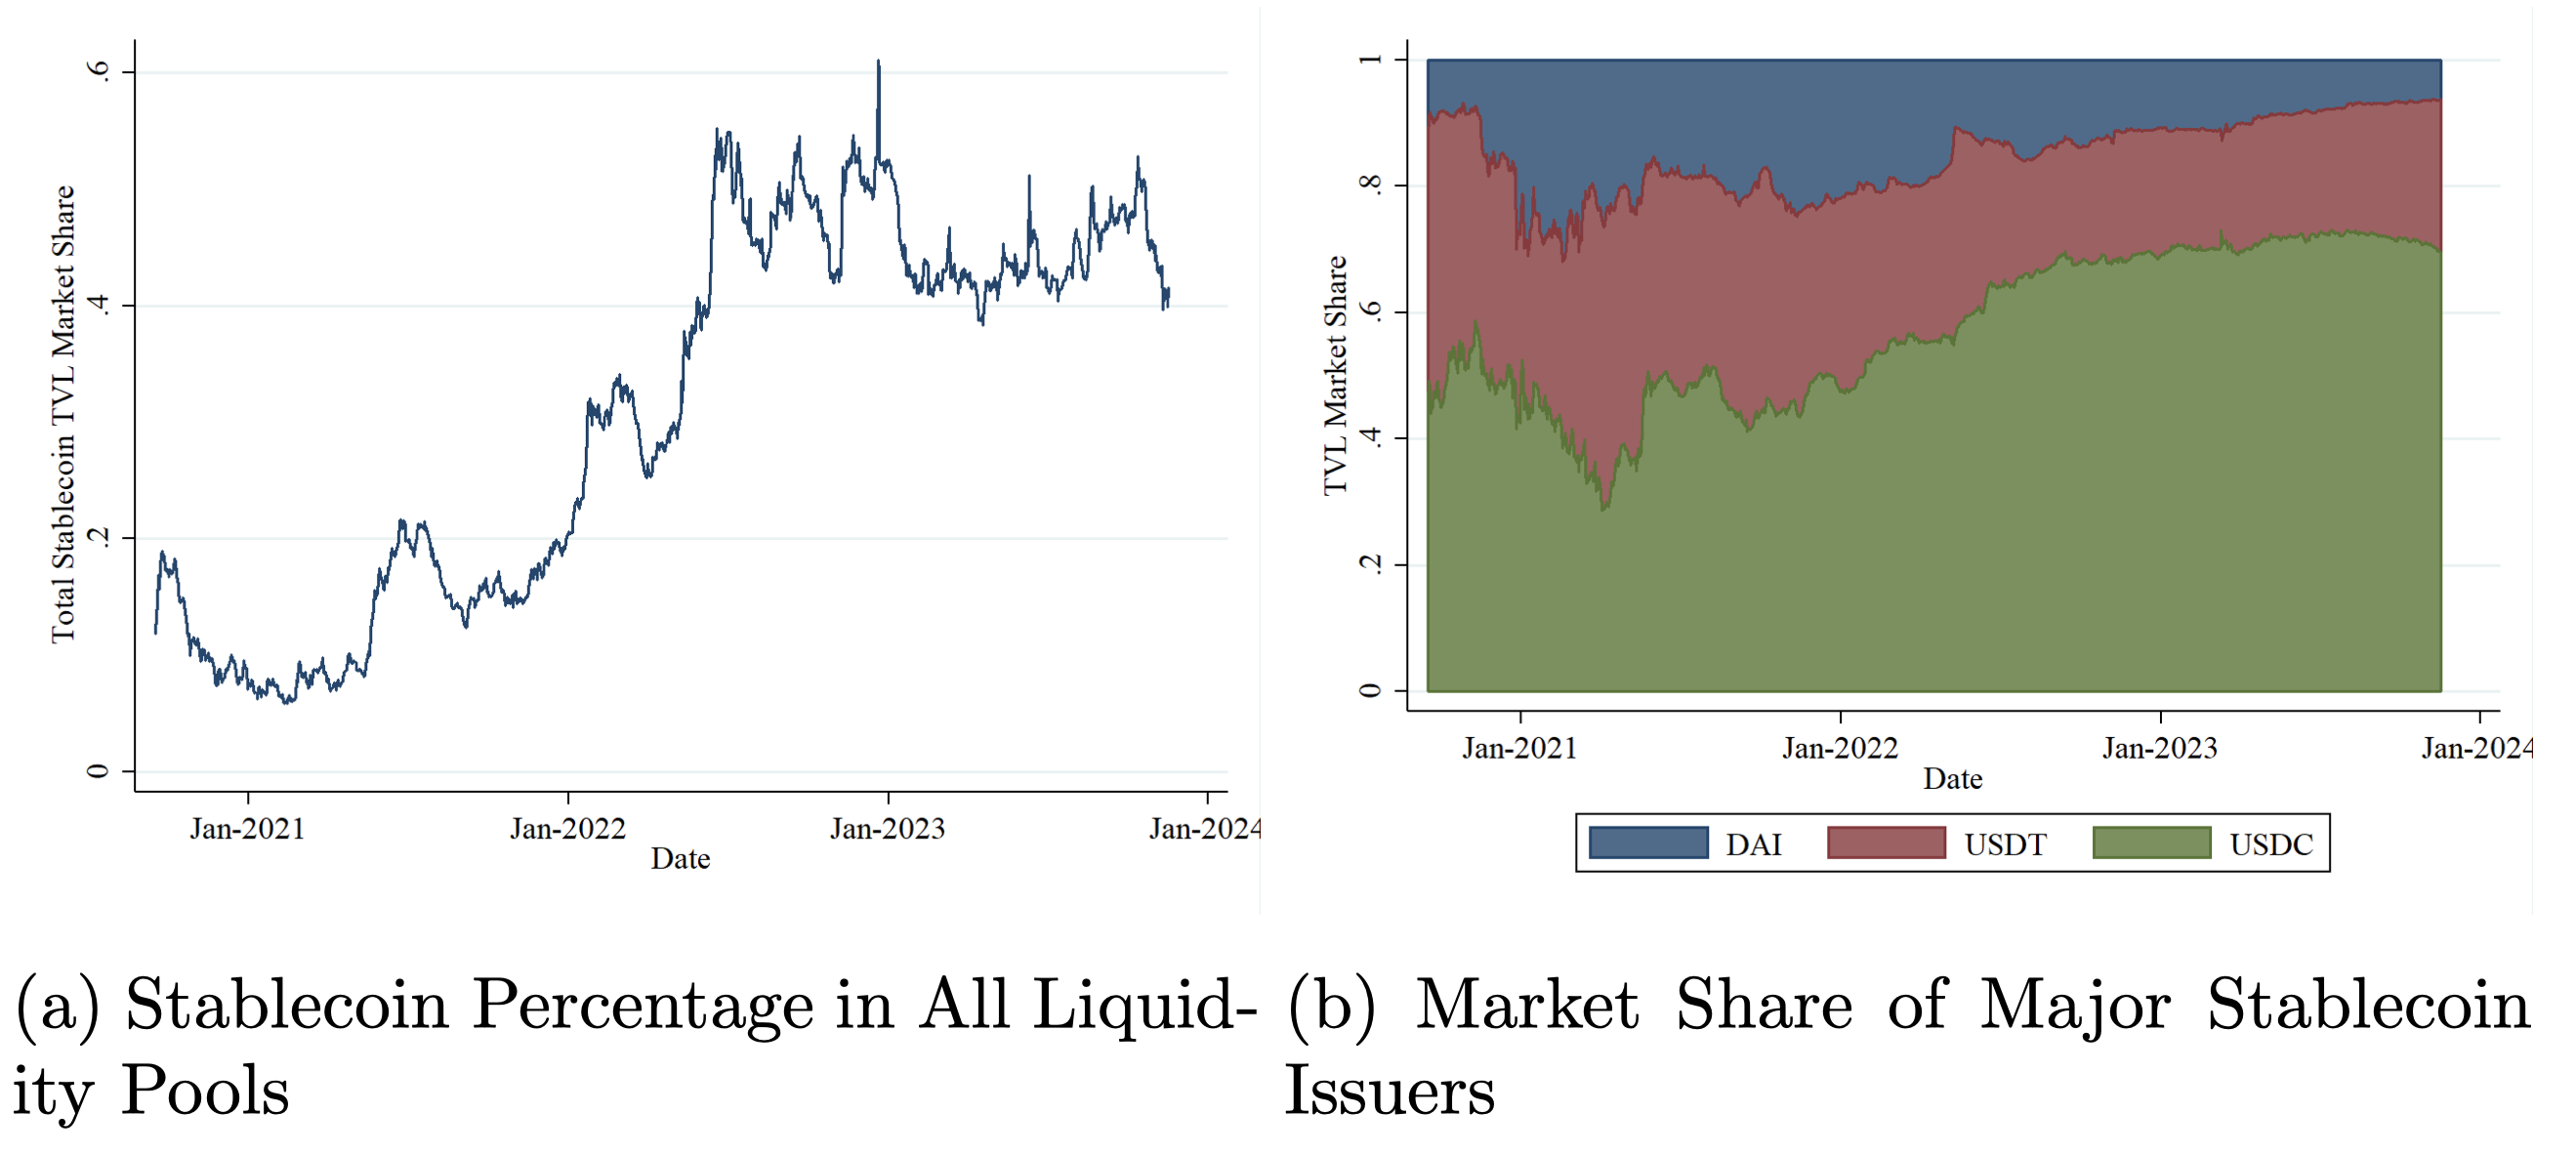
\includegraphics[width = \textwidth]{../Figures/stablecoins.png}
		\caption{Stablecoin collateral market share and concentration.}
	\end{figure}
\end{frame}
%%%

%%%
\begin{frame}{Oracle Network Dominance}
	\begin{figure}
		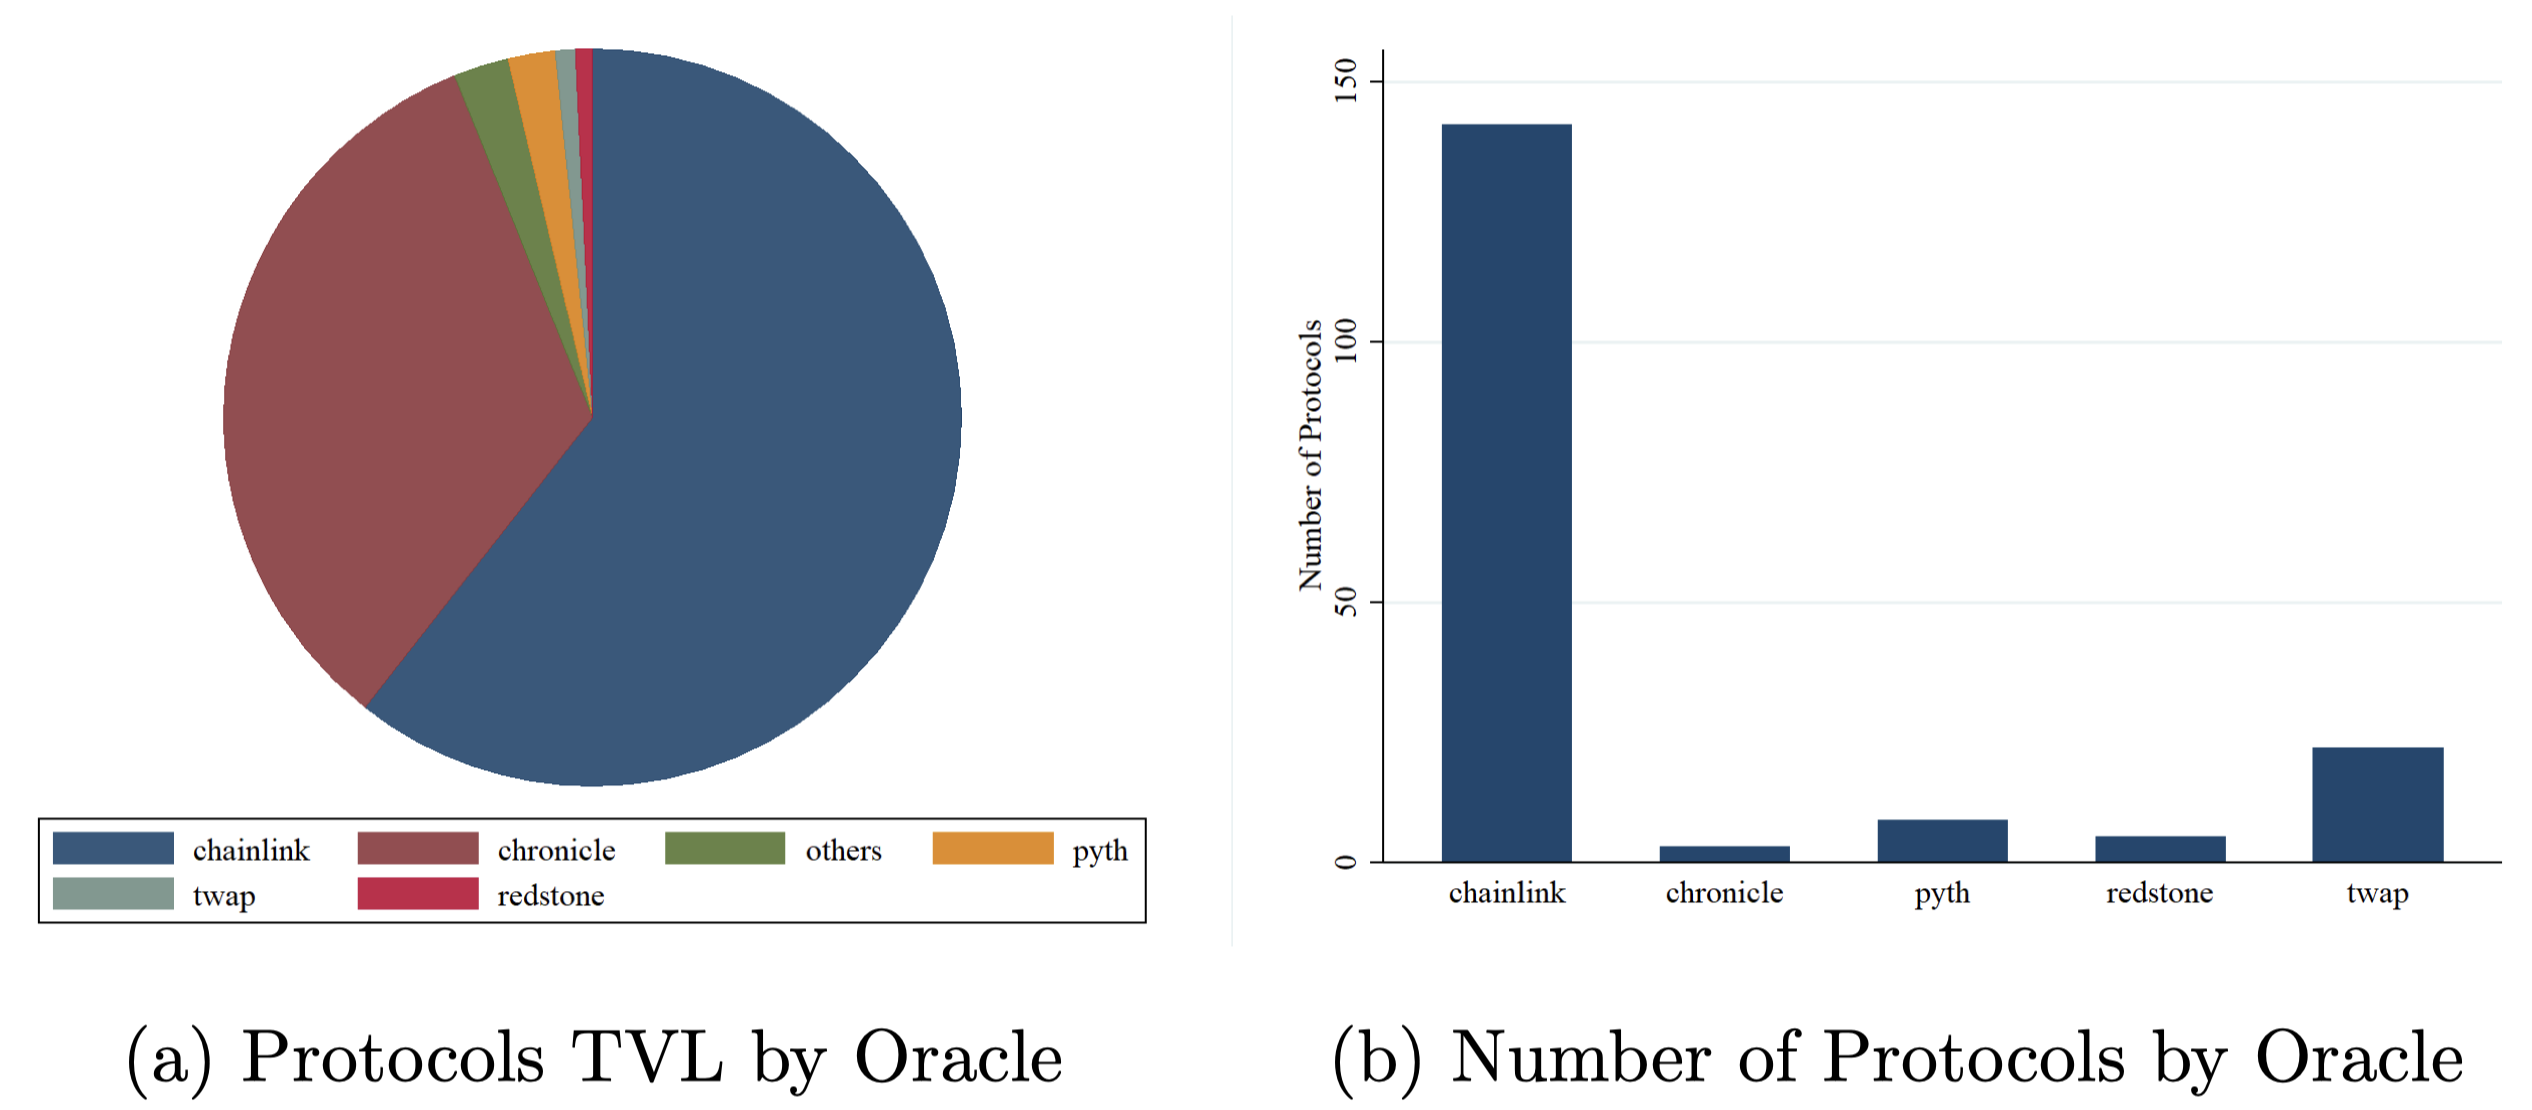
\includegraphics[width = \textwidth]{../Figures/oracleDominance.png}
		\caption{Oracle market share and protocols secured.}
	\end{figure}
\end{frame}
%%%


%%%%%%%%%%%%%%%%%%%%%%%%%%%%%%%%%%%%%%%%%%%%%
\section{Ethereum Governance and Token Price}
%%%%%%%%%%%%%%%%%%%%%%%%%%%%%%%%%%%%%%%%%%%%%
%%%

%%%
\begin{frame}{Ethereum Governance and Token Price}
	\begin{figure}
		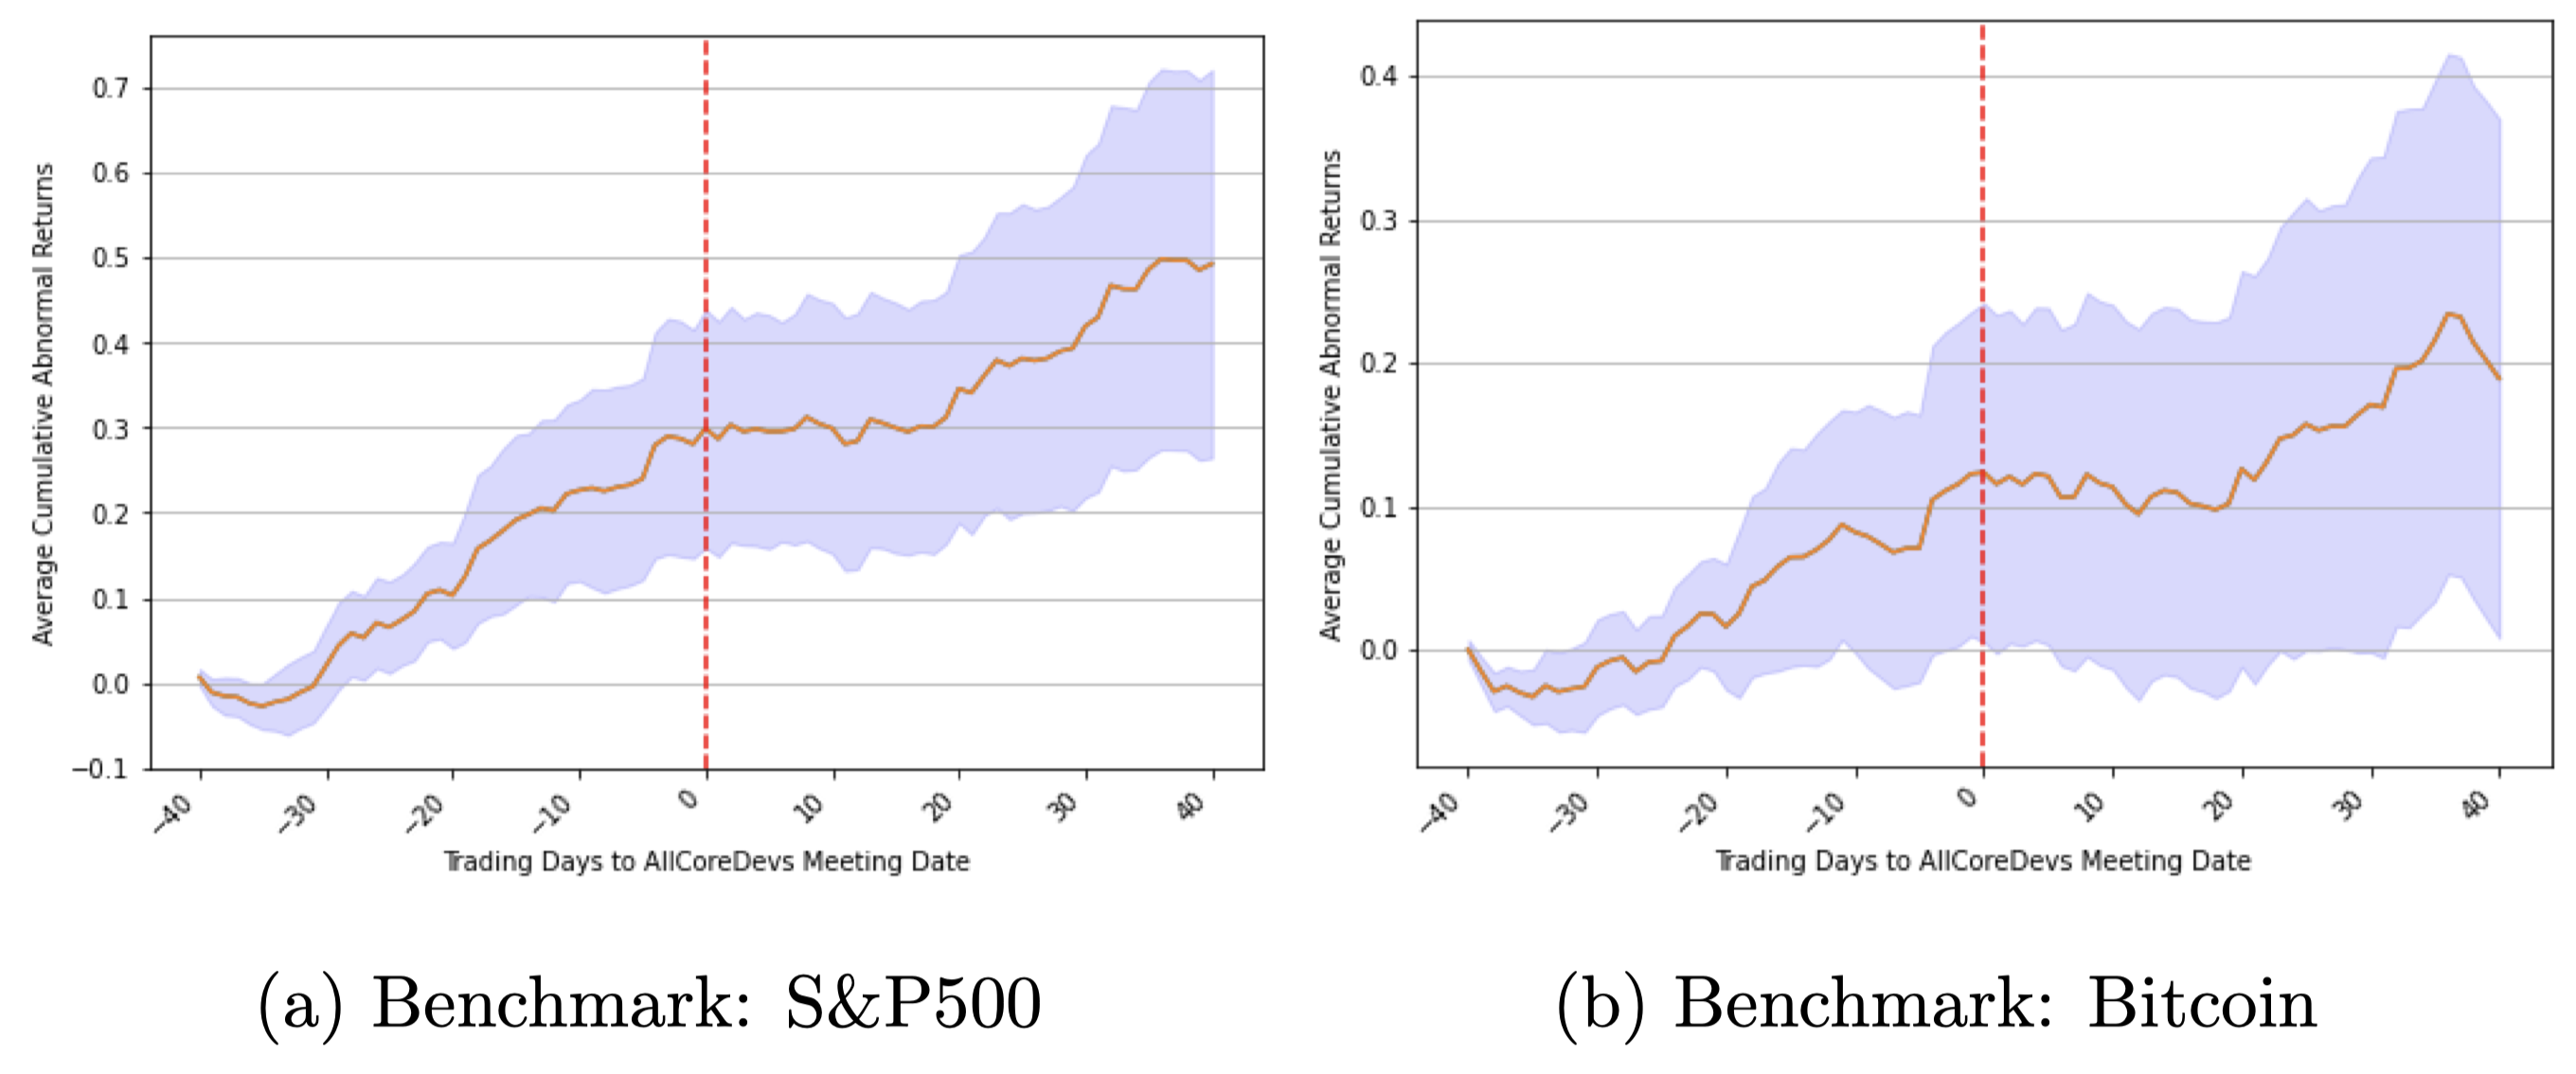
\includegraphics[width = \textwidth]{../Figures/tokenPrice.png}
		\caption{Cumulative abnormal returns (CARs) of Ether price in a $\left[-40,+40\right]$ trading day window around last AllCoreDevCall where the core EIP was discussed. $n=48$. Blue area = 0.9 confidence interval.}
	\end{figure}
\end{frame}
%%%



%%%%%%%%%%%%%%%%%%%%%%%%%%%%%%%%%%%%%%%%%%%%%%%%%%%%%%%%%%%%%%%%
\section{Conclusions}
%%%%%%%%%%%%%%%%%%%%%%%%%%%%%%%%%%%%%%%%%%%%%%%%%%%%%%%%%%%%%%%%

%%%
\begin{frame}{Conclusion}
	\begin{enumerate}
		\item Ethereum governance is a \textbf{complex} and \textbf{somewhat messy} process. 
		\item The relevant information is\textbf{ public}, and the \textbf{degree of transparency unprecedented}. 
		\item \textbf{Community involvement} is \textbf{large} and diverse. 
		\item Yet, the \textbf{core R\&D} activities are \textbf{centered around a relatively small number of people and entities through reverse dependency}
		\item Role of Ethereum Foundation is hard to capture quantitatively $\rightarrow$ \textbf{Soft power}.
        \item \textbf{ETH Token price is affected }by governance decisions.
	\end{enumerate}
\end{frame}
%%%

\end{document}
